
\begin{frame}\frametitle{\mirgecom{} V\&V defecit}
\begin{itemize}
\item We have some tests, both unit and integrated, full simulation tests
\item We have little (collective) knowledge about what capabilities are required for the prediction - we sometimes test with insufficient or irrelevant examples
\item Lack of knowledge about what is tested, and what tests we have, and how good they are, and what they test frustrates the prediction effort
\end{itemize}
\end{frame}


% \begin{frame}\frametitle{\pyrometheus{}~~~~~~~~~~~~~~~~~~~~~~~~~~~\prj{\tiny}{Esteban Cisneros}}
%  \begin{itemize}
%  \item Package for thermochemistry-code generation
%    \begin{itemize}
%    \item Uses Cantera to handle mechanism parameterization, and for verification
%    \item Based on \textbf{code template}, \textbf{automatic diff.} $\rightarrow$ facilitate extensions
%    \end{itemize}
%  \item Freely-available: \url{https://github.com/ecisneros8/pyrometheus}
%  \end{itemize}
%
%  \begin{itemize}
%  \item Applications:
%    \begin{itemize}
%    \item Reacting-flow simulations: \textit{PlasCom2}, \textit{MirgeCOM}
%    \item Mechanism design
%    \item Chemical model reduction and uncertainty quantification\\
%      \tiny{\sPI{Cisneros--Garibay, Pantano \& Freund,} \textit{Combust. Flame} (2019)}
%    \end{itemize}
%  \end{itemize}
%  \begin{center}
%  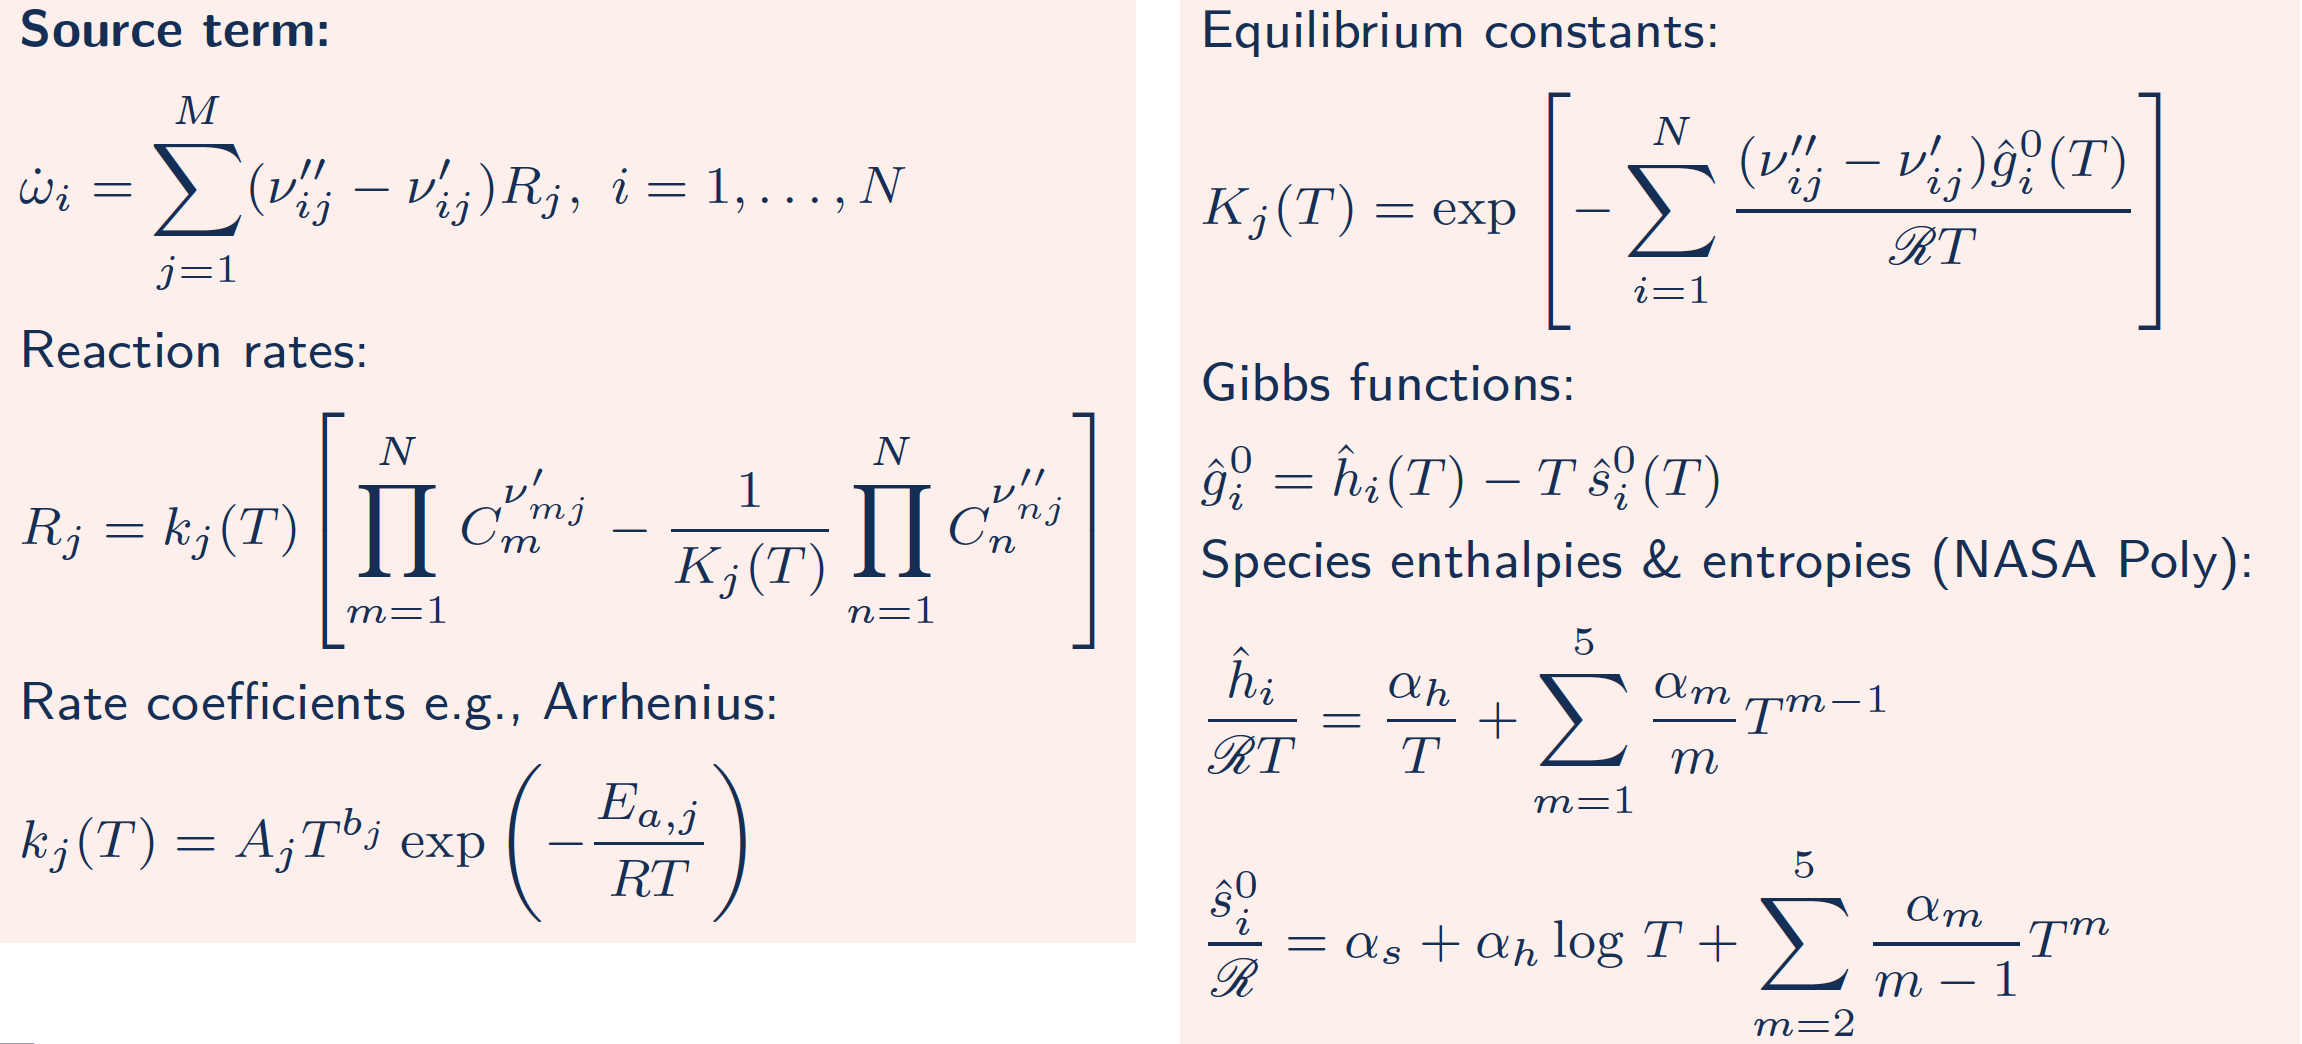
\includegraphics[width=.8\textwidth]{figures/PyroStuff.png}
%  \end{center}
%  \begin{center}
%   \end{center}
%\end{frame}

\begin{frame}\frametitle{\pyrometheus{}~~~~~~~~~~~~~~~~~~~~~~~~~~~\prj{\tiny}{Esteban Cisneros}}
\begin{itemize}
  \item Thermo + kinetics verified against \textit{Cantera}
  \item Illustration: 32-species ethylene mechanism \tiny{\sPI{Luo et al.,,} \textit{Combust. Flame} (2012)}\normalsize
  \item Full verification suite provided with distribution
\end{itemize}
  \begin{center}
  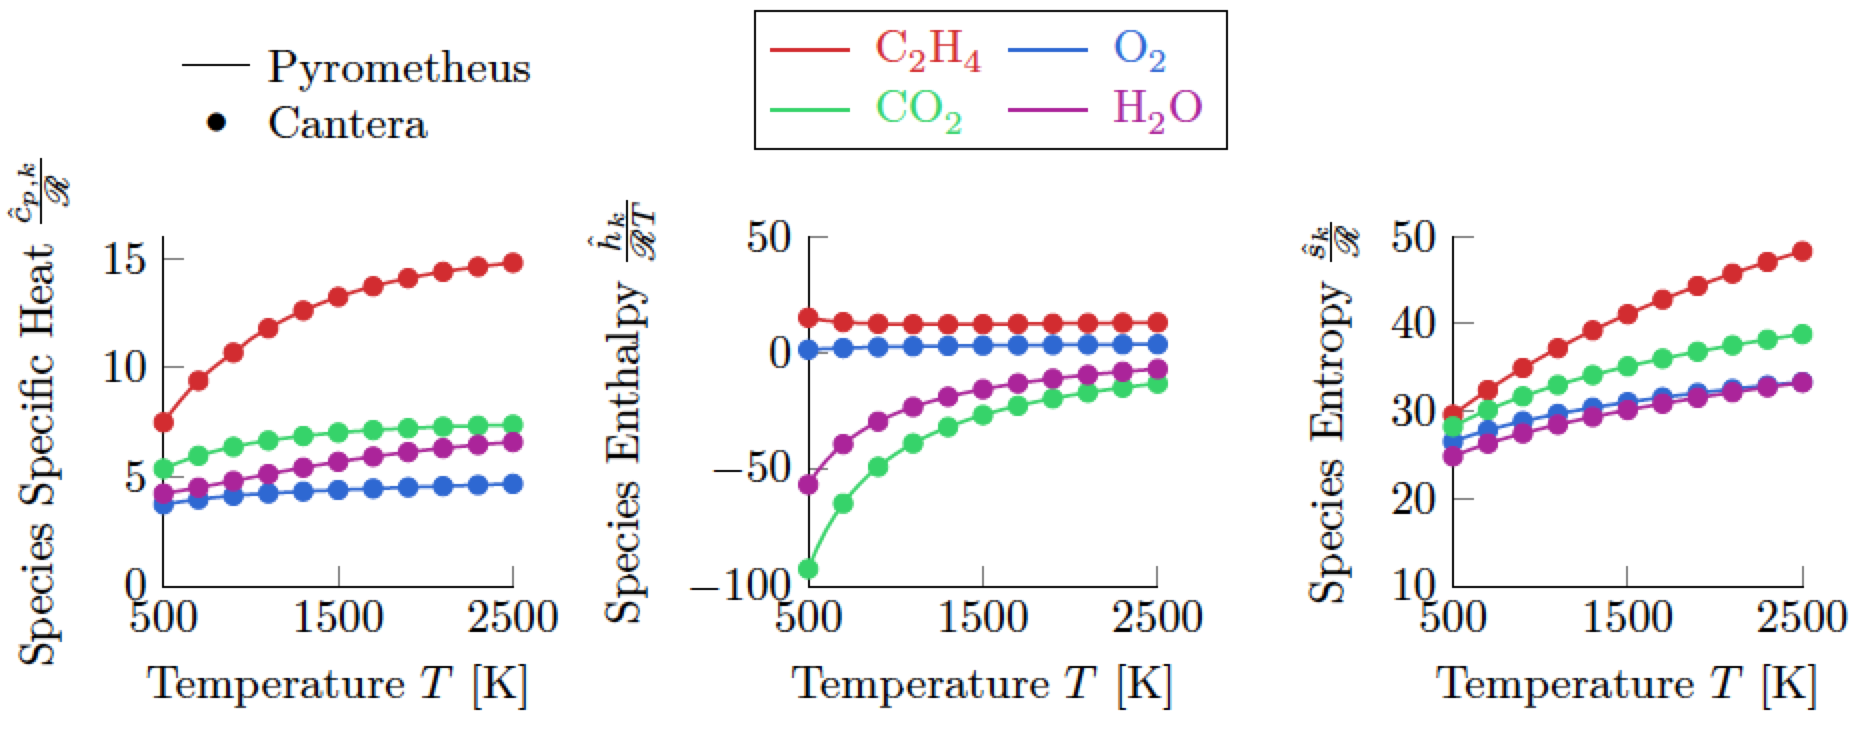
\includegraphics[width=.7\textwidth]{figures/PyroVerif1.png}\\
  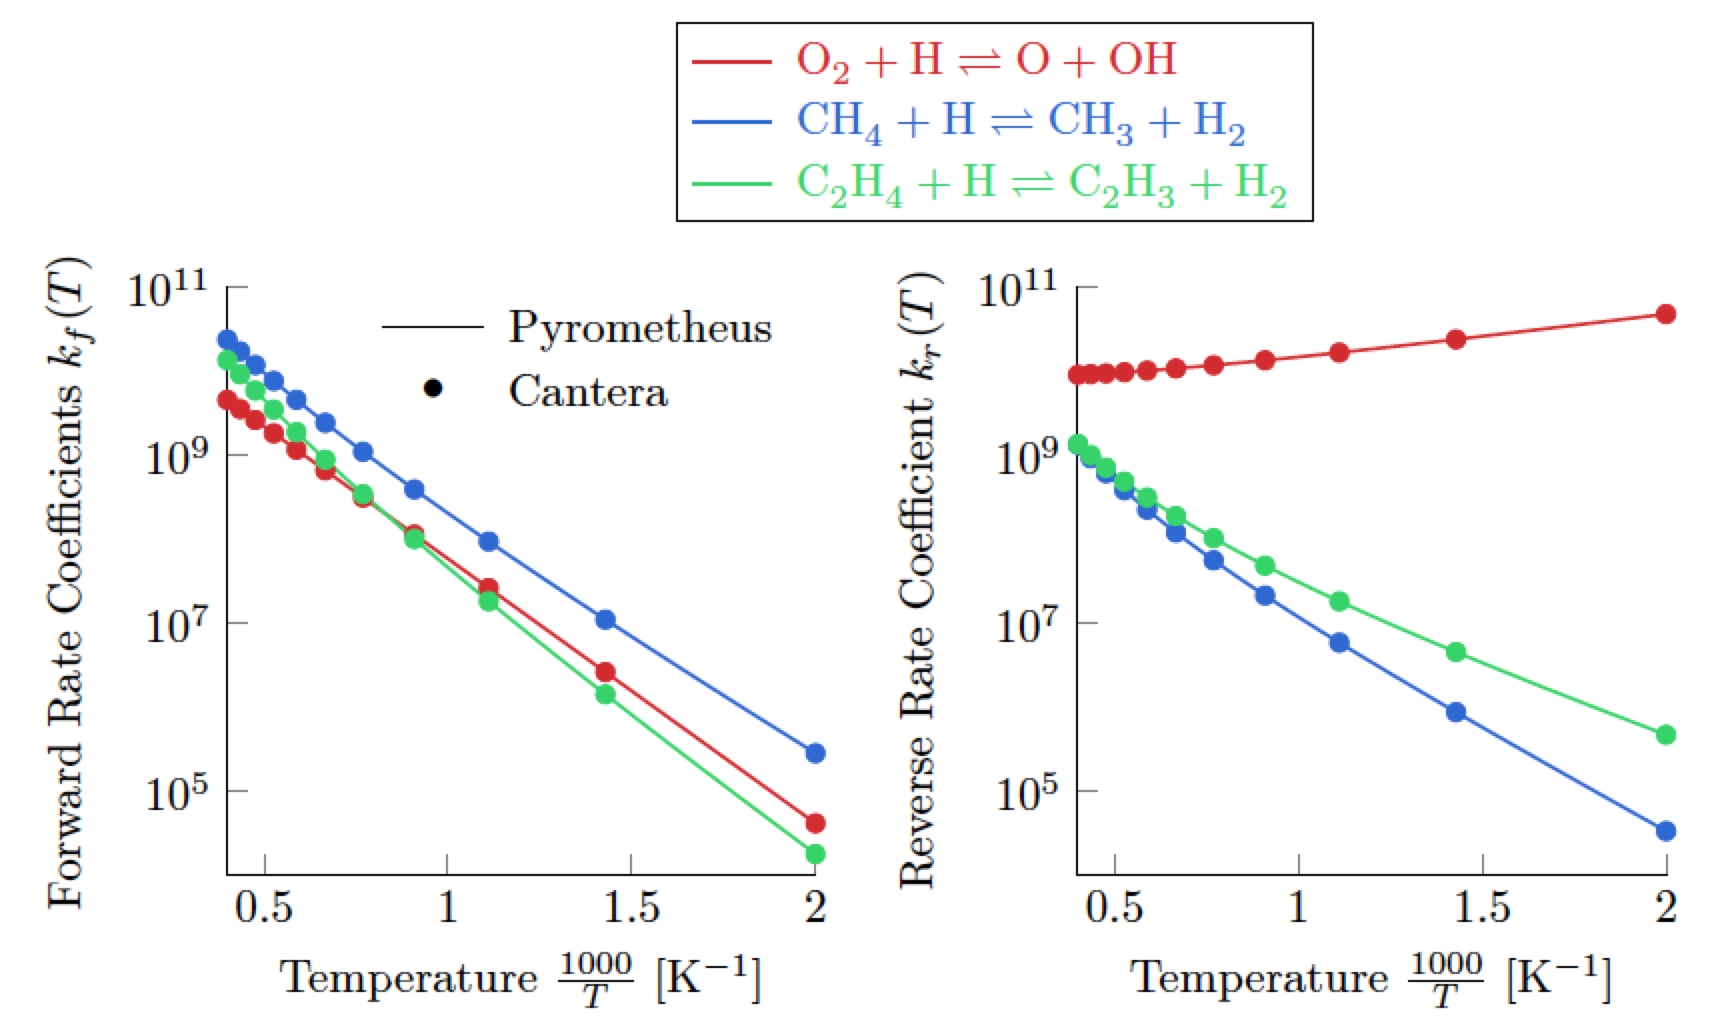
\includegraphics[width=.5\textwidth]{figures/PyroVerif2.png}
  \end{center}
%  \begin{center}
%      \prj{\tiny}{Esteban Cisneros}
%   \end{center}
\end{frame}

% \begin{frame}\frametitle{\pyrometheus{} $\rightarrow$ \mirgecom}
%  \begin{multicols}{2}
%%    \begin{itemize}
%%    \item \textit{Prometheus}
%      \begin{itemize}
%      \item \pyrometheus{} inline-generates thermochem code for \mirgecom 
%      \item Uses \textit{Cantera} and generates Python
%      \item \textit{Cantera} added as a required TPL
%      \item \textit{Cantera} CTI files to add new mechanisms
%      \end{itemize}
%      \columnbreak
%%    \item \pyrometheus
%    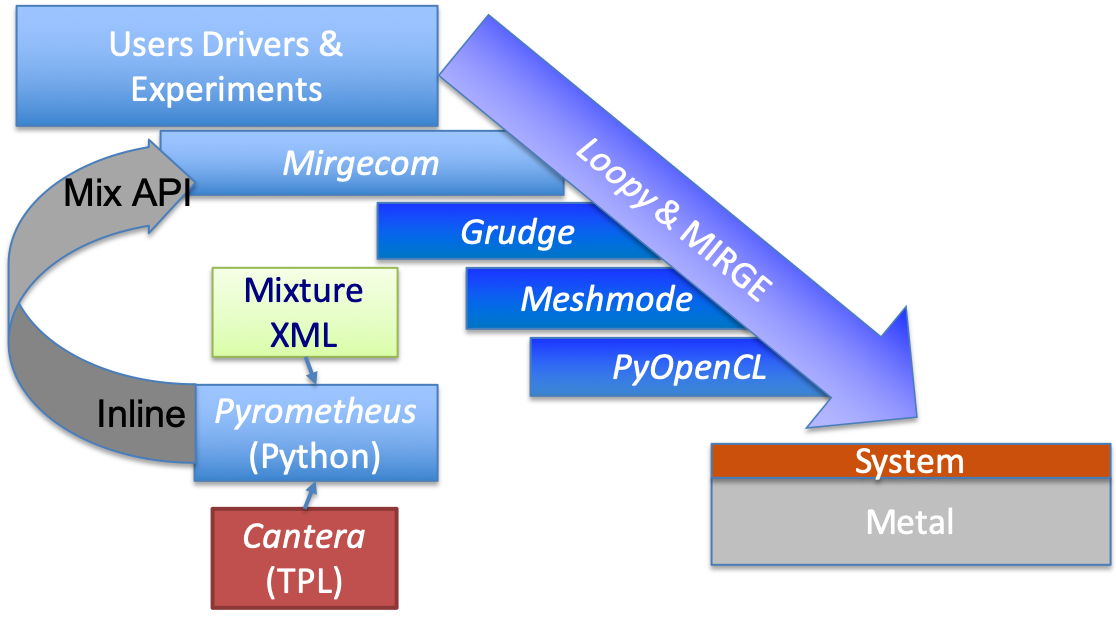
\includegraphics[width=.5\textwidth]{figures/mtc/PyrometheusIntegration.png}
%    \vspace{-20pt}
%%    \end{itemize}
%  \end{multicols}
%  \vspace{-15pt}
%  \begin{multicols}{2}
%    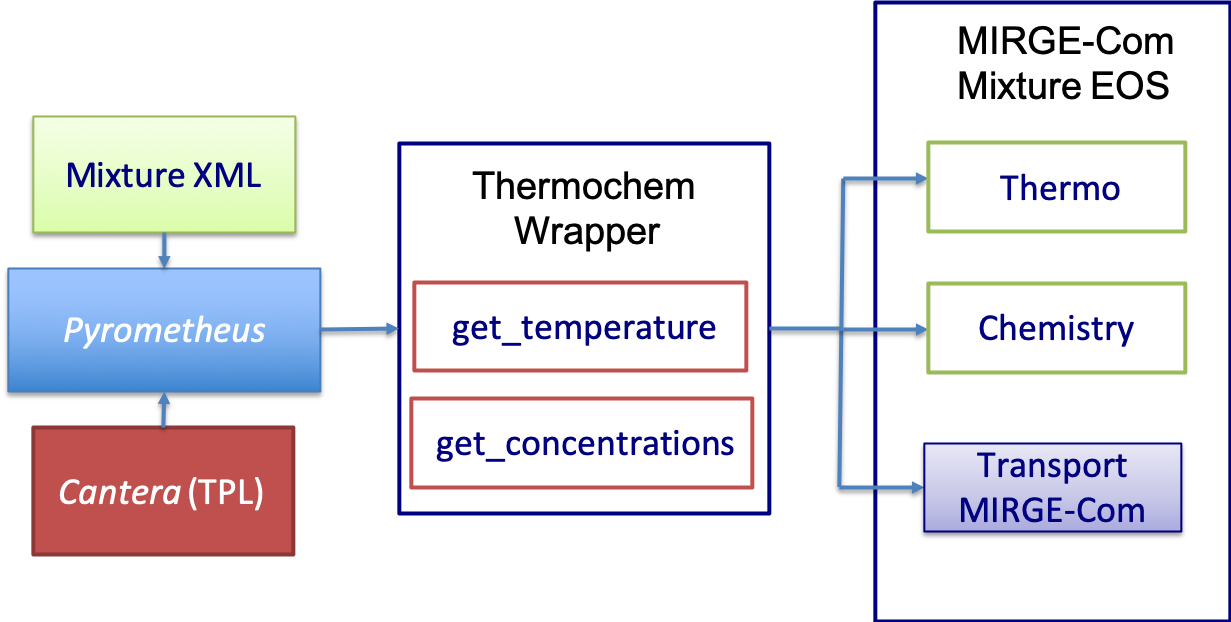
\includegraphics[width=.5\textwidth]{figures/PyroIntegrationWrapper.png}\\
%      \columnbreak
%    \begin{itemize}
%      \vspace{-20pt}
%      \item \mirgecom{} wrapper (\texttt{thermochemistry.py})
%      \item \mirgecom{} MixtureEOS (\texttt{eos.py})
%      \item \pyrometheus{} test suite (\texttt{test\_eos.py})
%      \end{itemize}
%  \end{multicols}
%\end{frame}

%\begin{frame}\frametitle{\pyrometheus{} in \mirgecom}
%\begin{center}
% Autoignition co-verification
%\end{center}
%\begin{itemize}
%   \item Ethylene/air mixture $(1500\mathtt{K}, \rho=\mathtt{const})$
%   \item \pyrometheus-predicted profiles match \textit{Cantera}
%   \item \pyrometheus{} with implicit time integration with \textit{CVODE}
%   \item \mirgecom{} with RK4, inviscid, quiescent
%\end{itemize}
%\begin{multicols}{2}
%    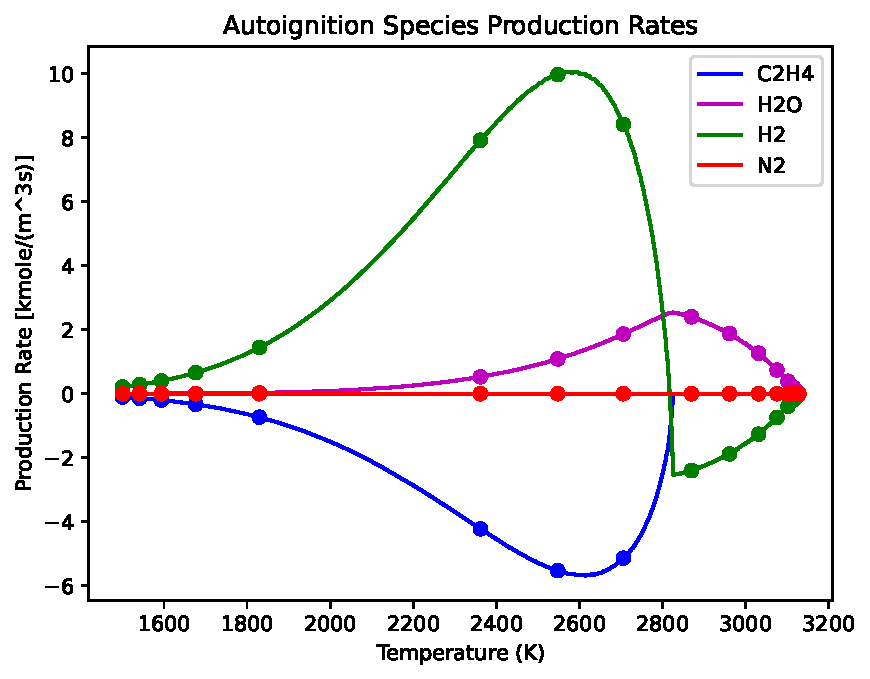
\includegraphics[width=.45\textwidth]{figures/autoignition_rates.pdf}\\
%    \columnbreak
%    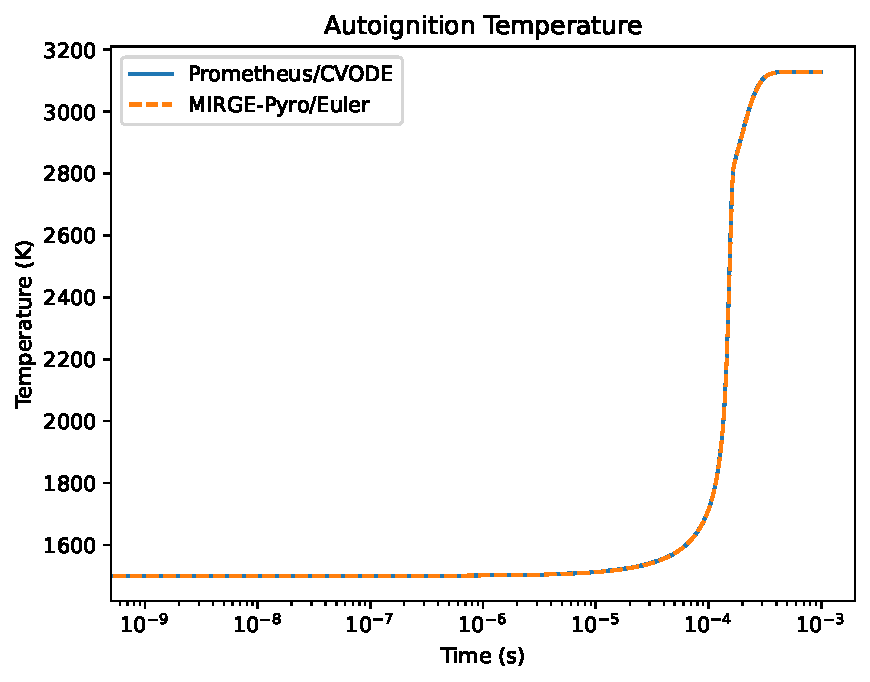
\includegraphics[width=.45\textwidth]{figures/autoignition_temperature.pdf}
%  \end{multicols}
%\end{frame}


% MIRGE performance stuff
\begin{frame}\frametitle{Combozzle: scalable test case}
  \begin{minipage}{0.45\textwidth}		
    \begin{itemize}
    \item Y2-adjacent (fluid-only) physics (NS, AV, sponge)
    \item Bozzle + optional mixture/combustion
    \item RK4 time integrator, UIUC mech
    \end{itemize}
    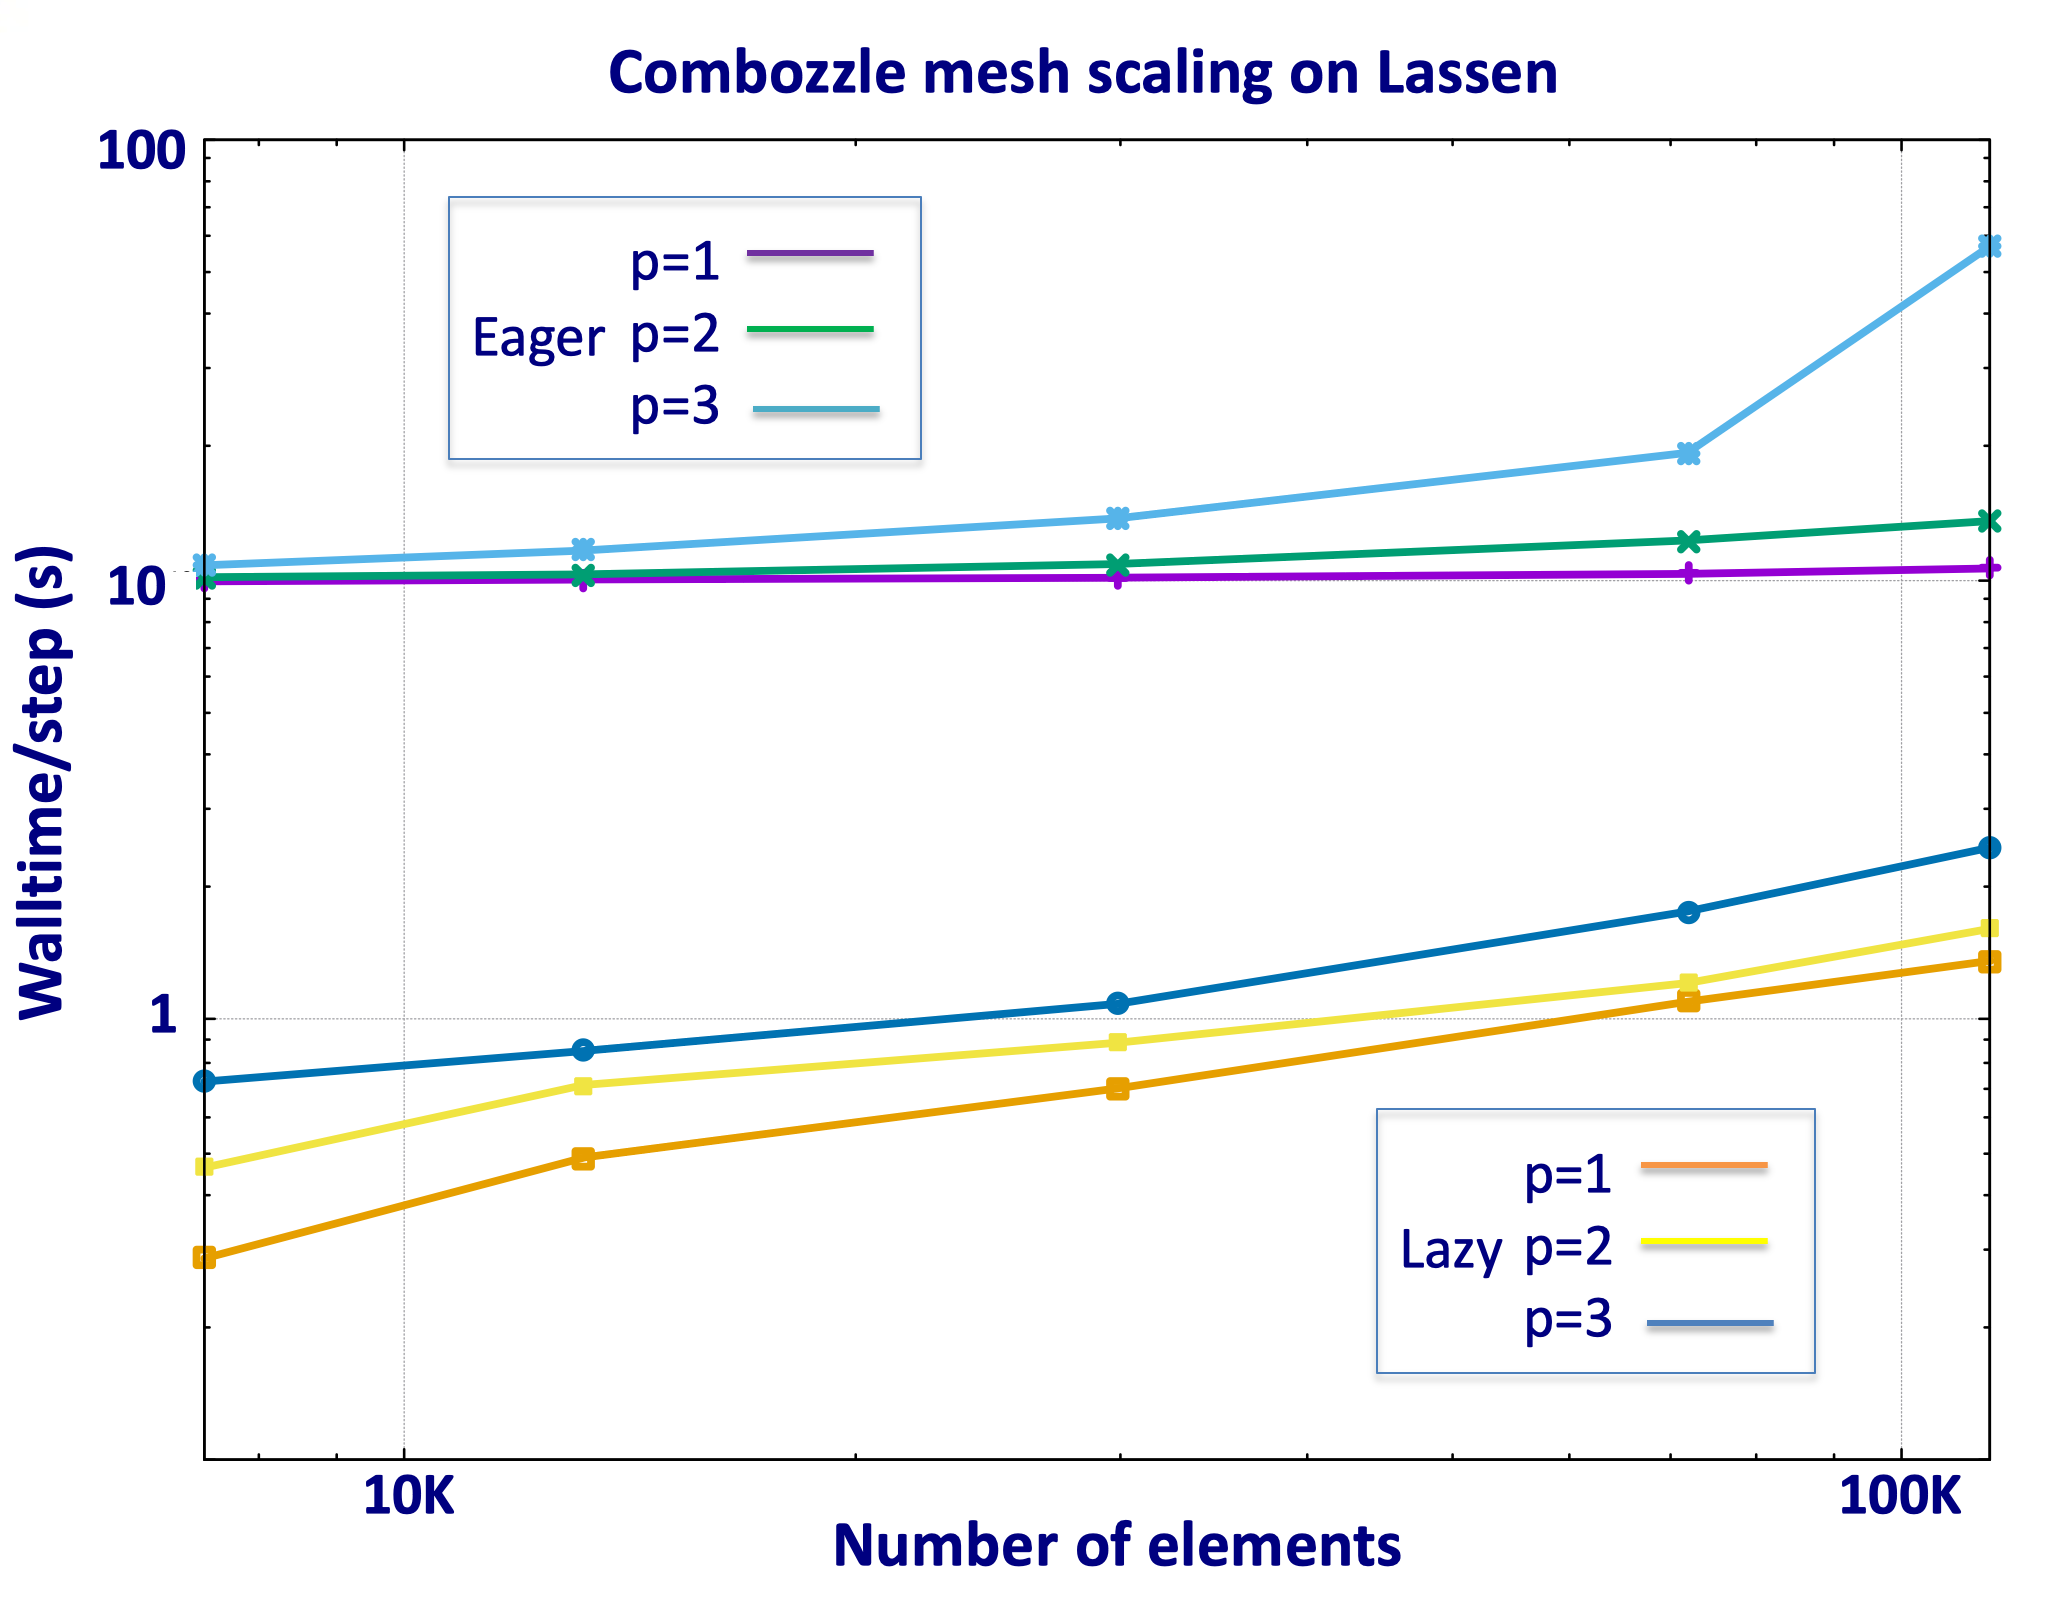
\includegraphics[width=\textwidth]{figures/combozzle_gridscale.png}
  \end{minipage}
  \begin{minipage}{0.5\textwidth}
    \begin{figure}
      \centering
      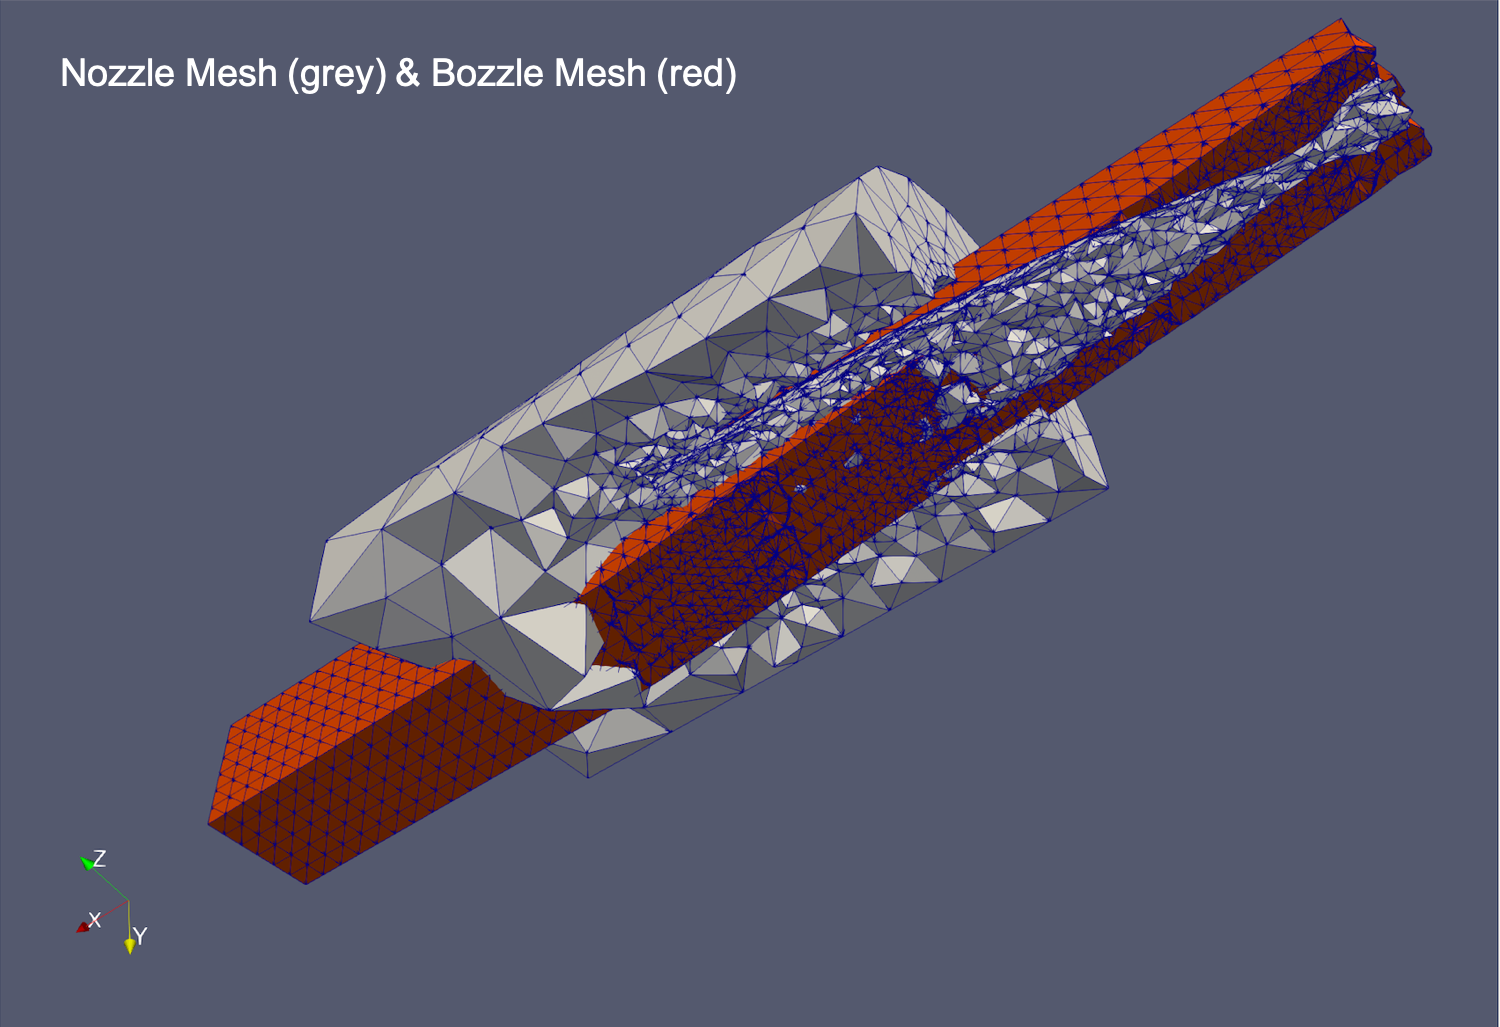
\includegraphics[width=\textwidth]{figures/bono2.png} \\
      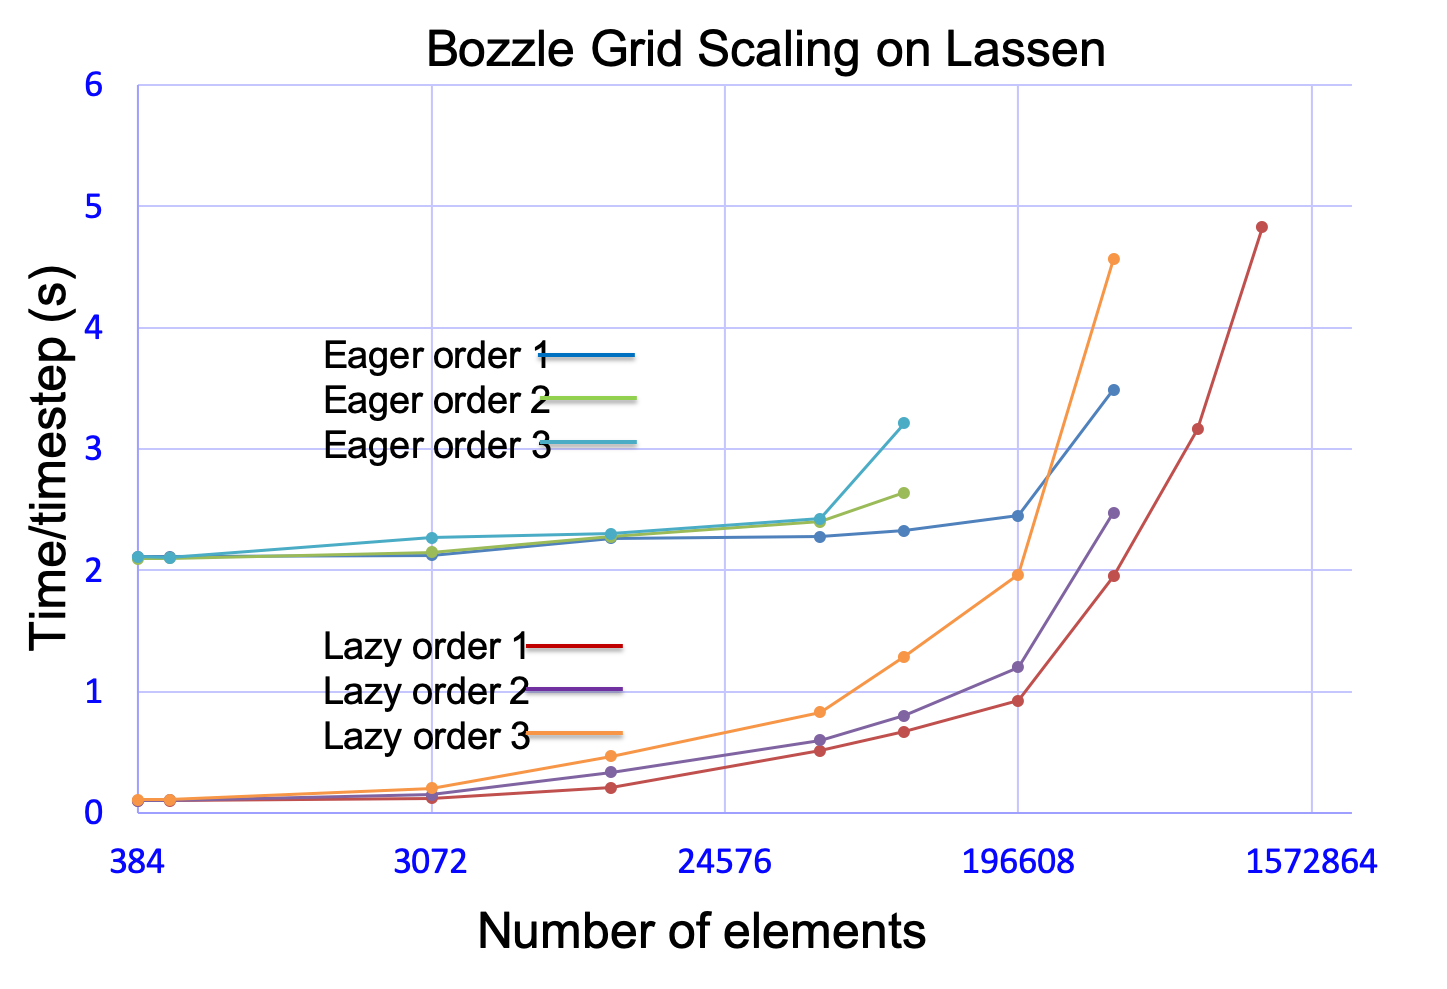
\includegraphics[width=\textwidth]{figures/bozzle_gridscale.png}
    \end{figure}		
  \end{minipage}
\end{frame}

\begin{frame}\frametitle{Expected performance?}
\begin{itemize}
\item Flop counting lazy is challenging
\item DG is a local scheme: Expect linear in number of elements
\item Expect linear in number of RHS calls
\end{itemize}
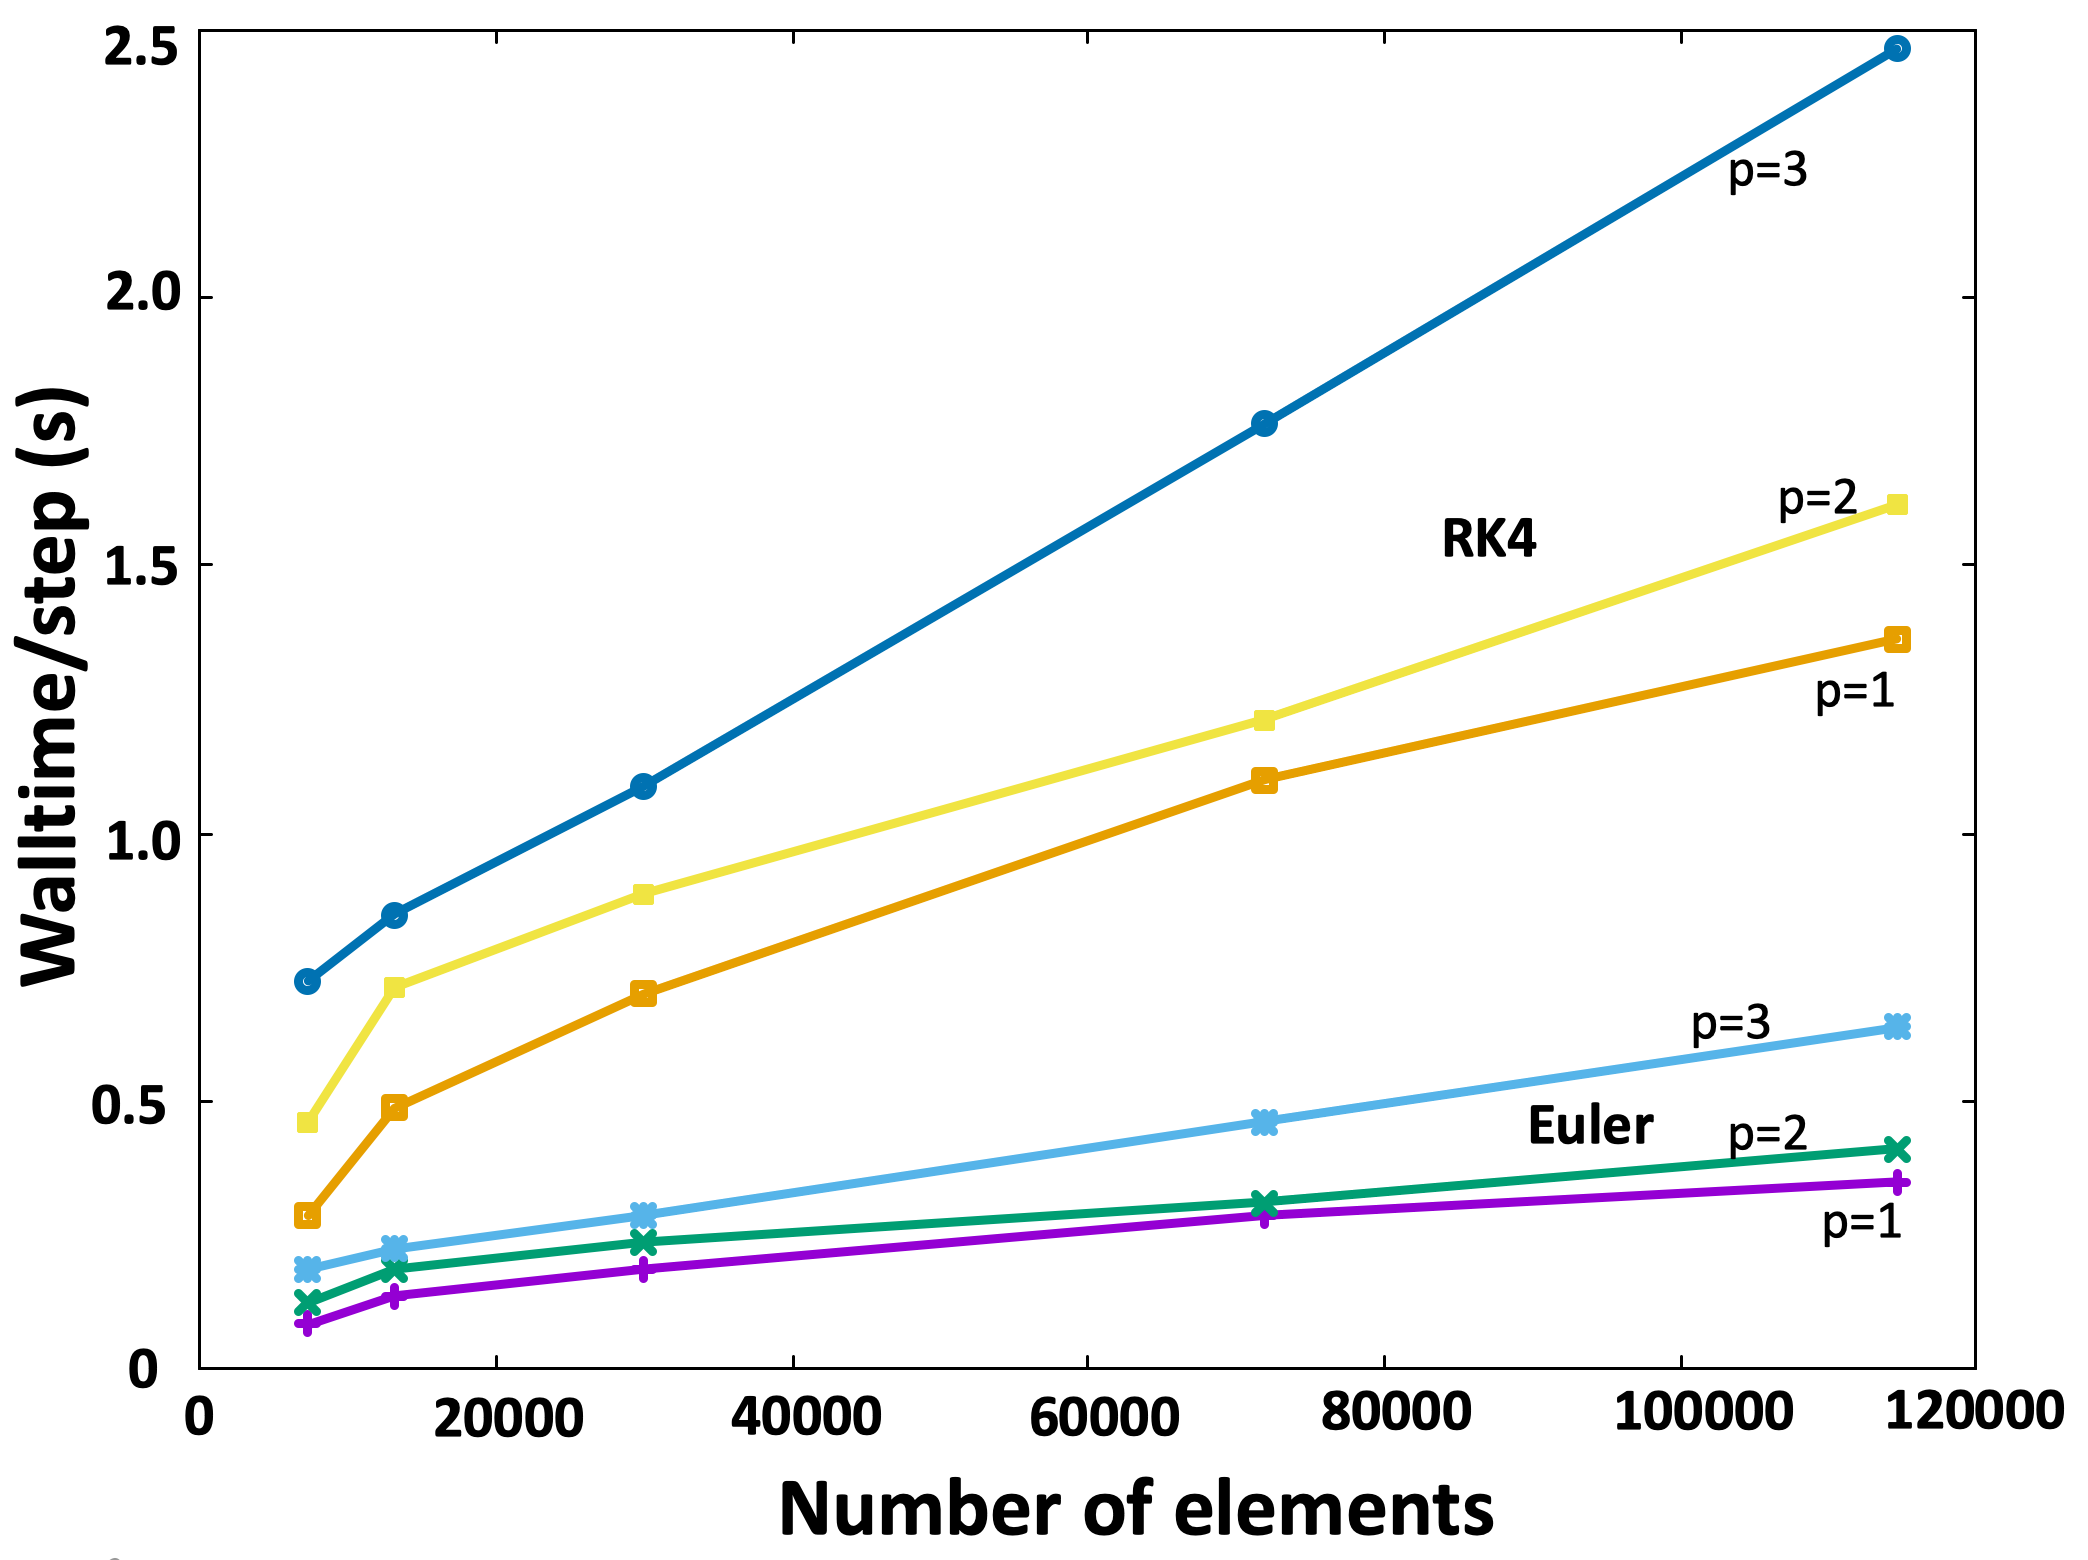
\includegraphics[width=.45\textwidth]{figures/TSCompare.png}
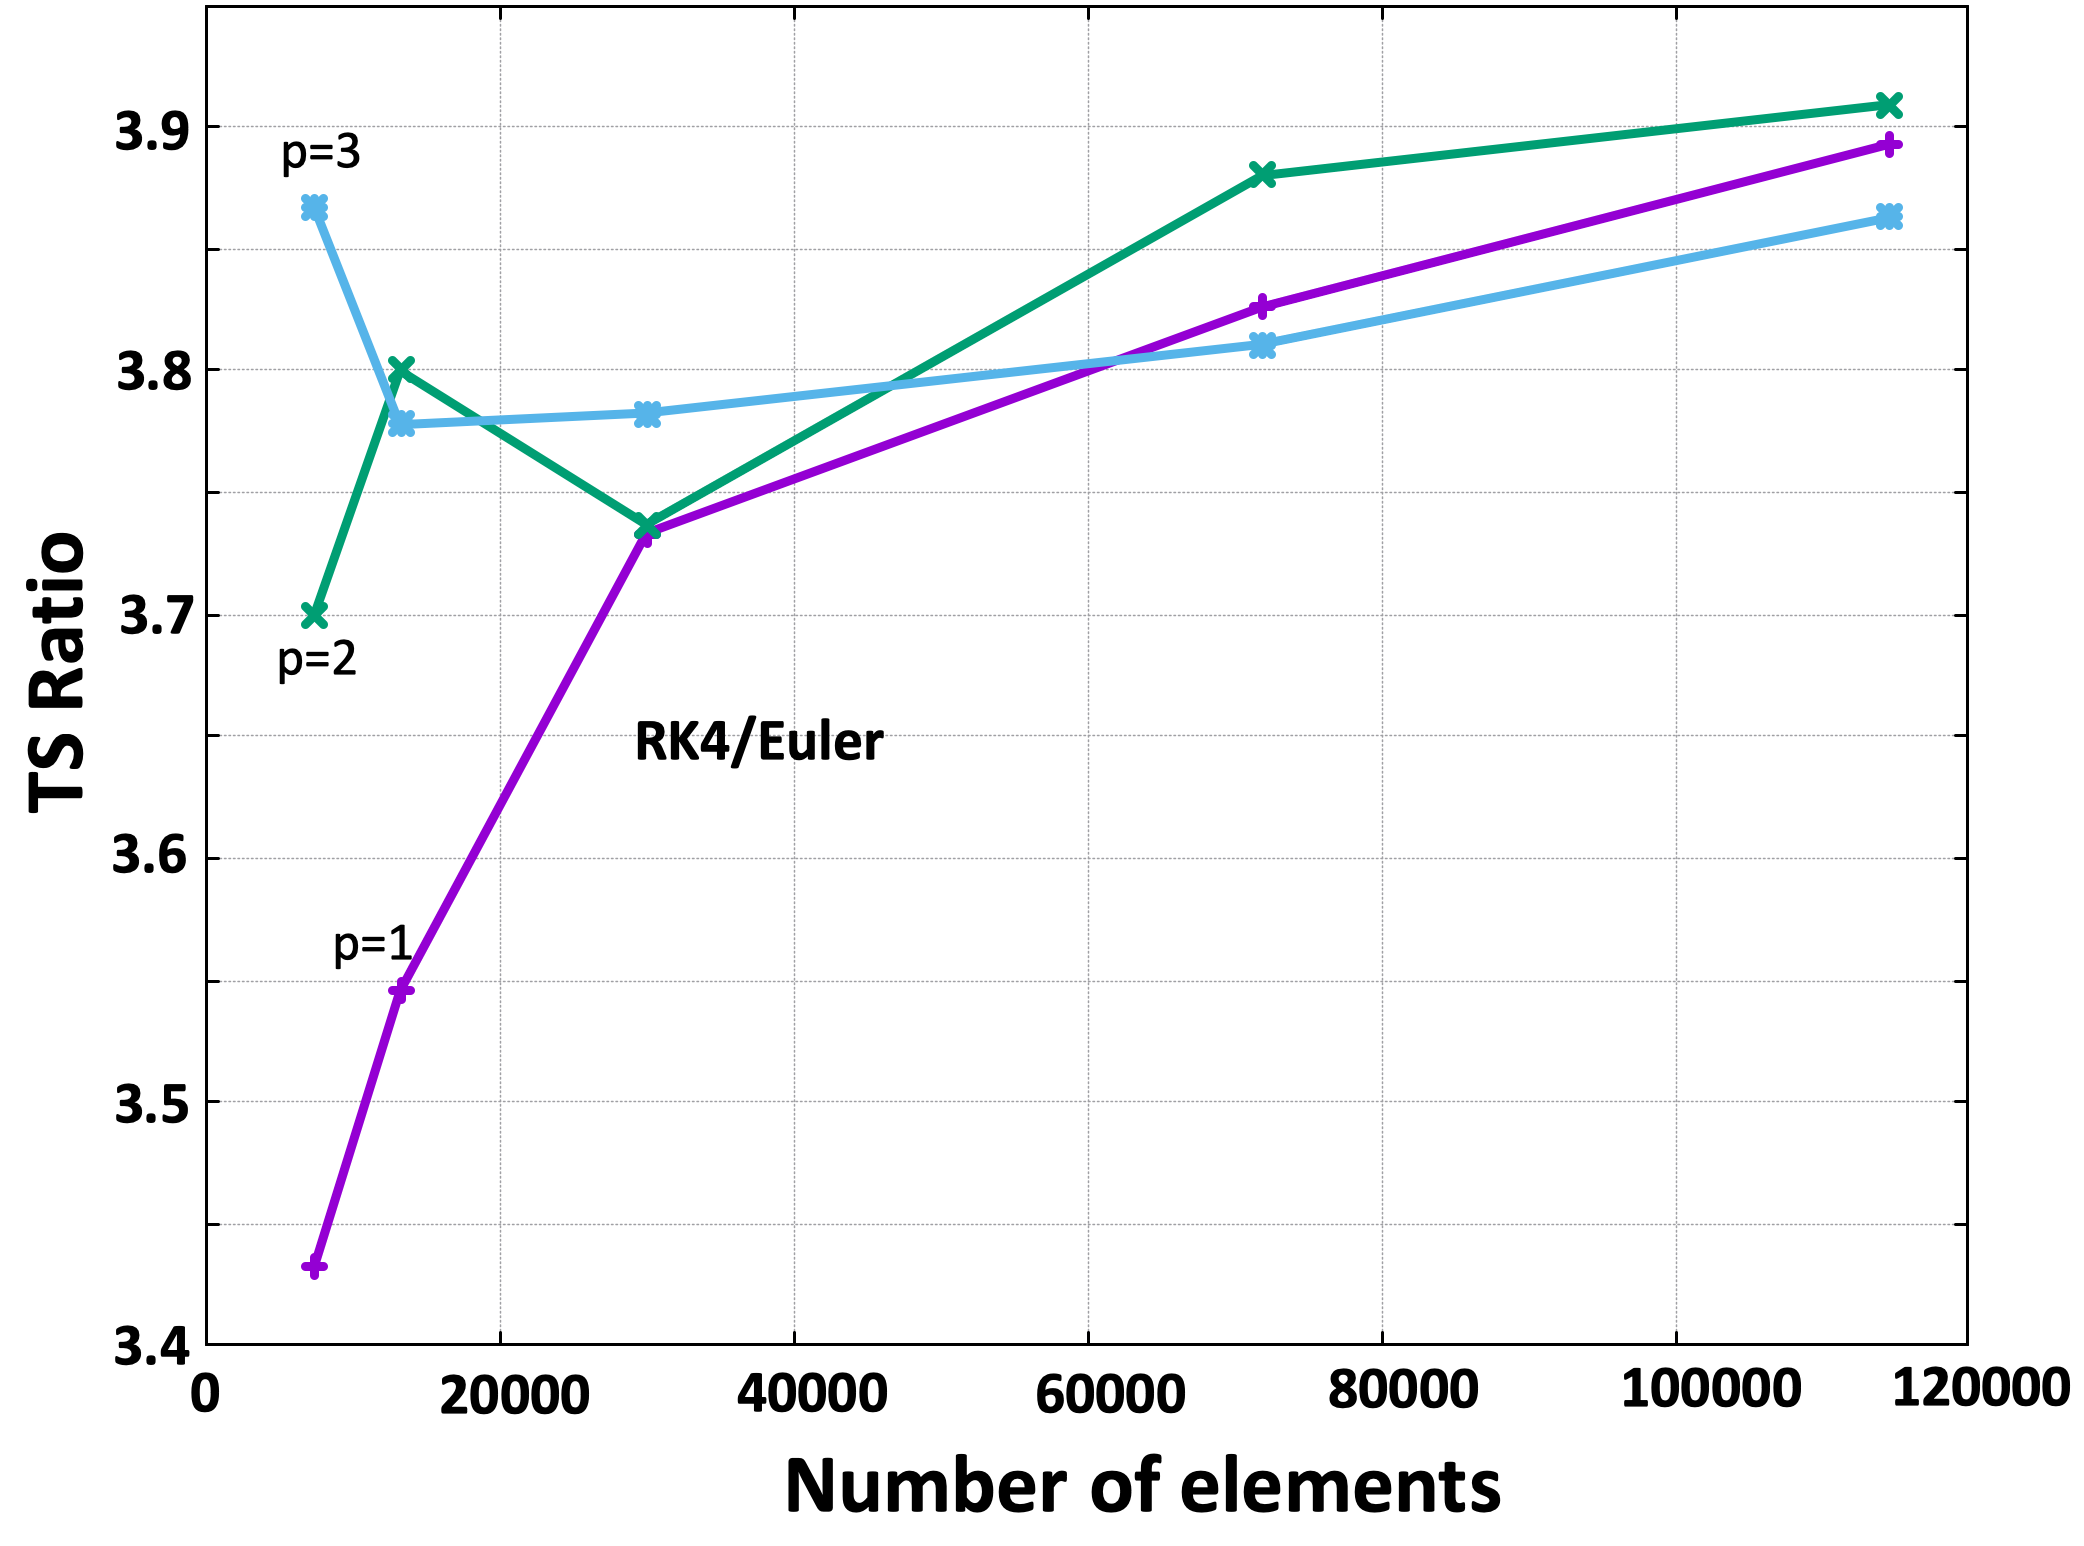
\includegraphics[width=.45\textwidth]{figures/TSRatio.png}
\end{frame}

% AK-sanctioned rip-off 
\begin{frame}\frametitle{DG - The program}
  \begin{multicols}{2}
    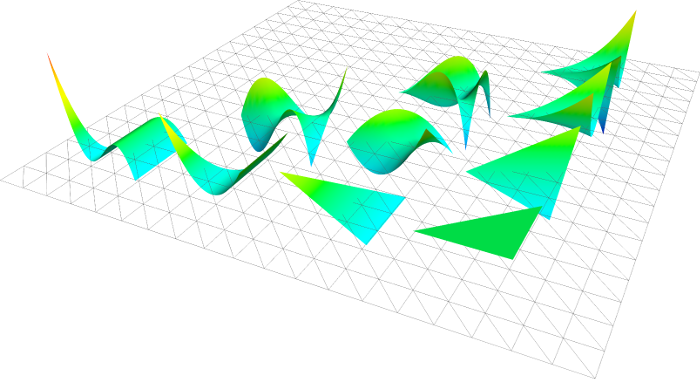
\includegraphics[width=0.4\textwidth]{figures/pkdo-2d.png}
    \vspace{-10pt}
   \newcommand{\meshnodes}{
  \coordinate (a) at (4.53,2.86) ;
  \coordinate (b) at (2.91,3.55) ;
  \coordinate (c) at (2.25,1.8) ;
  \coordinate (d) at (-0.3,3.25) ;
  \coordinate (e) at (1.31,4.17) ;
  \coordinate (f) at (1.19,0.43) ;
  \coordinate (g) at (2.77,0.7) ;
  \coordinate (h) at (3.96,3.54) ;
  \coordinate (i) at (0.05,1.17) ;
  \coordinate (j) at (2,3.1) ;
  \coordinate (k) at (3,4.7) ;
  \coordinate (m) at (3.93,1.65) ;
  \coordinate (n) at (1.78,0.76) ;
  \coordinate (o) at (0.40,4.4) ;
  \coordinate (p) at (0.8,2.5) ;
  \coordinate (q) at (4.72,1.32) ;
  \coordinate (r) at (3.02,2.27) ;
  \coordinate (s) at (0.98,1.83) ;
  \coordinate (t) at (-0.3,1.8) ;
}


\newcommand{\withmeshtris}[1]{
  #1 cgn #1 snf #1 jsc #1 pjs
  #1 pts #1 sif #1 sit #1 dtp
  #1 odp #1 epj #1 jcb #1 oep
  #1 rcg #1 crb #1 kbh #1 rah
  #1 ejb #1 rgm #1 ram #1 qam
  #1 ekb #1 gqm #1 scn #1 bhr
}

\newcommand{\drawtriangle}[3]
  {\draw (#1) -- (#2) -- (#3) -- cycle;}
\newcommand{\meshtris}{
  \withmeshtris\drawtriangle
}
\def\drawnodenames{
  \foreach \i in {a,b,c,d,e,f,g,h,i,j,k,m,n,o,p,q,r,s,t}
    \node at (\i) {\i};
}
  

    \begin{tikzpicture}[scale=0.4]
      \meshnodes
      \meshtris
      \draw [fill=blue!30] (c) -- (n) -- (g) ;
      \node [left=10mm of g,xshift=-2mm] (ellabel) {$E_k$};
      \draw [thick,->,shorten >=2mm] (ellabel) -- (c) ;
    \end{tikzpicture}
    \vspace{-10pt}
    \prj{\tiny}{Kl{\"o}ckner}\columnbreak \\
    Numerical approximation to $\mathbf{Q}$, $\mathbf{S}$:
    \begin{equation*}
      \partial_t\mathbf{q}^{*} + \nabla \cdot \mathbf{F}(\mathbf{q}^{*}) - \mathbf{s}^{*} = 0
    \end{equation*}
    Hit with test function and integrate over element:
    \begin{equation*}
      \int_{E_k}[(\partial_t\mathbf{q}^{*} - \mathbf{s}^{*}) + (\nabla \cdot \mathbf{F}(\mathbf{q}^{*}))]\phi\,dx = 0
    \end{equation*}
  \end{multicols}
  \begin{center}
    Integrate by parts:
    \begin{equation*}
      \int_{E_k}(\partial_t\mathbf{q}^{*}- \mathbf{s}^{*})\phi\,dx -
      \int_{E_k}(\mathbf{F}(\mathbf{q}^{*}) \cdot \nabla{\phi})\,dx +
      \int_{\partial{E_k}}(\hat{n} \cdot \mathbf{F}(\mathbf{q}^{*}))\phi\,dx
    \end{equation*}
  \end{center}
  \begin{center}
    Rearranging in matrix form:
    \begin{equation*}
      \mathcal{M}[\partial_t\mathbf{q}^{*}] = \mathcal{M}[\mathbf{s}^{*}] + ( \mathcal{S}[\mathbf{F}(\mathbf{q}^{*})] )
      - \sum{\mathcal{M}_{\partial{E_k}}[(\hat{\mathbf{n}} \cdot \mathbf{f}^{*})]} ) 
    \end{equation*}
  \end{center}
\end{frame}

\begin{frame}\frametitle{Expected performance?}
\begin{itemize}
\item Flop counting lazy is challenging
\item DG is a local scheme: Expect linear in number of elements
\item Expect linear in number of RHS calls
\end{itemize}
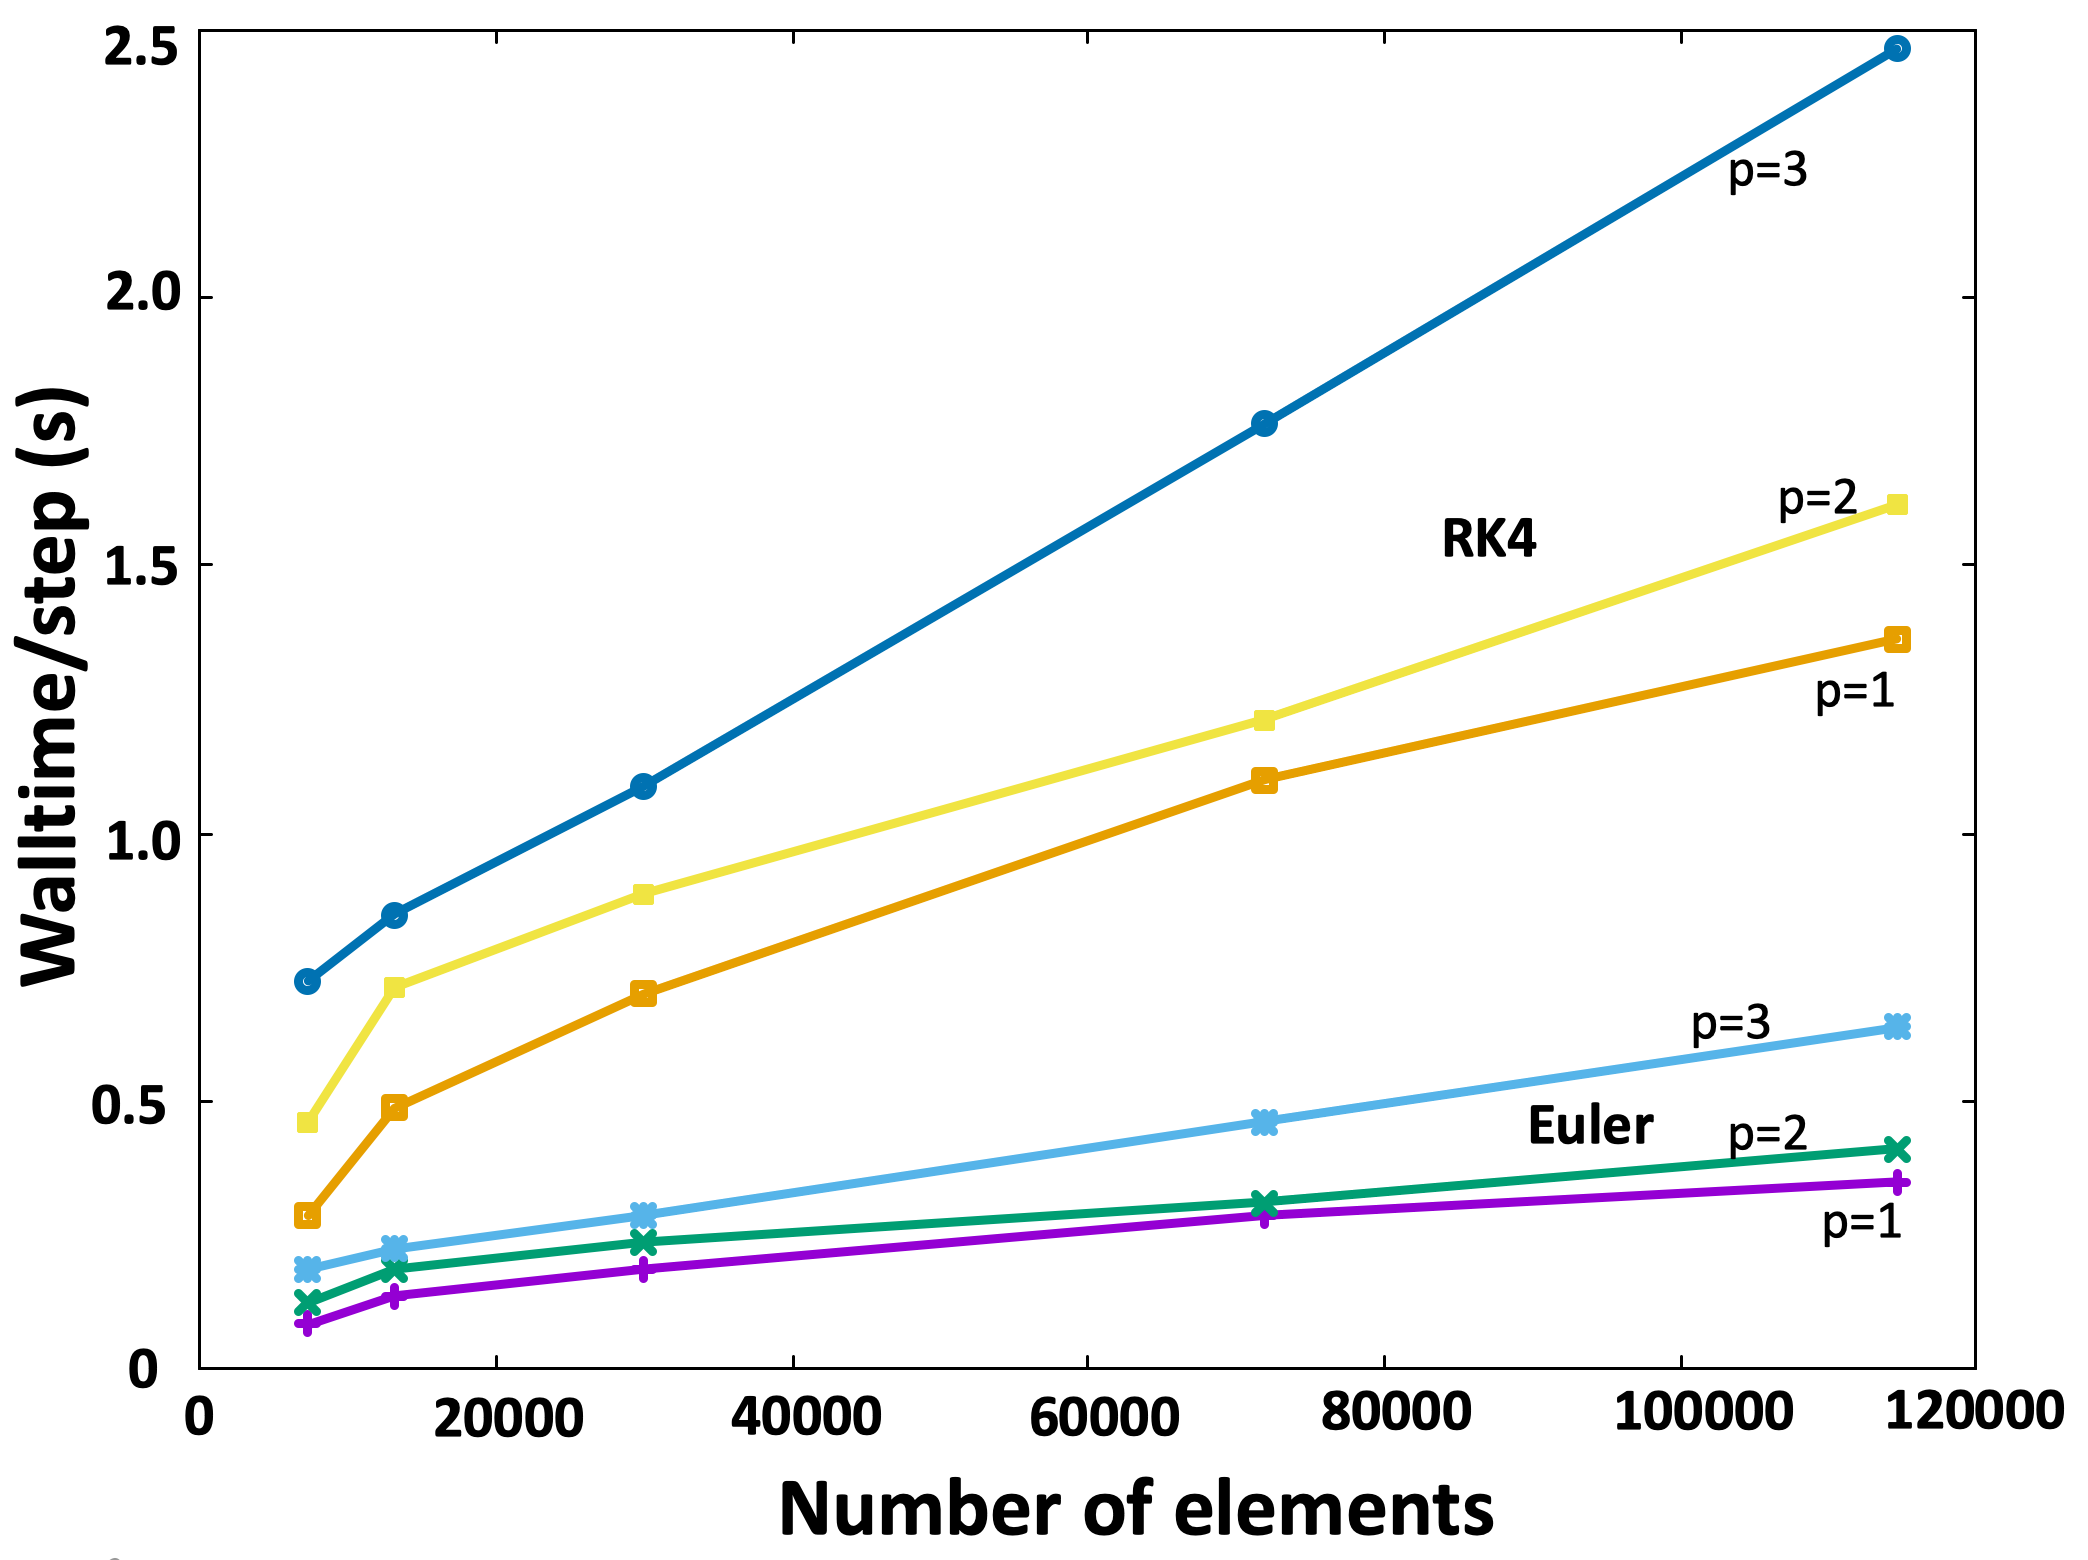
\includegraphics[width=.45\textwidth]{figures/TSCompare.png}
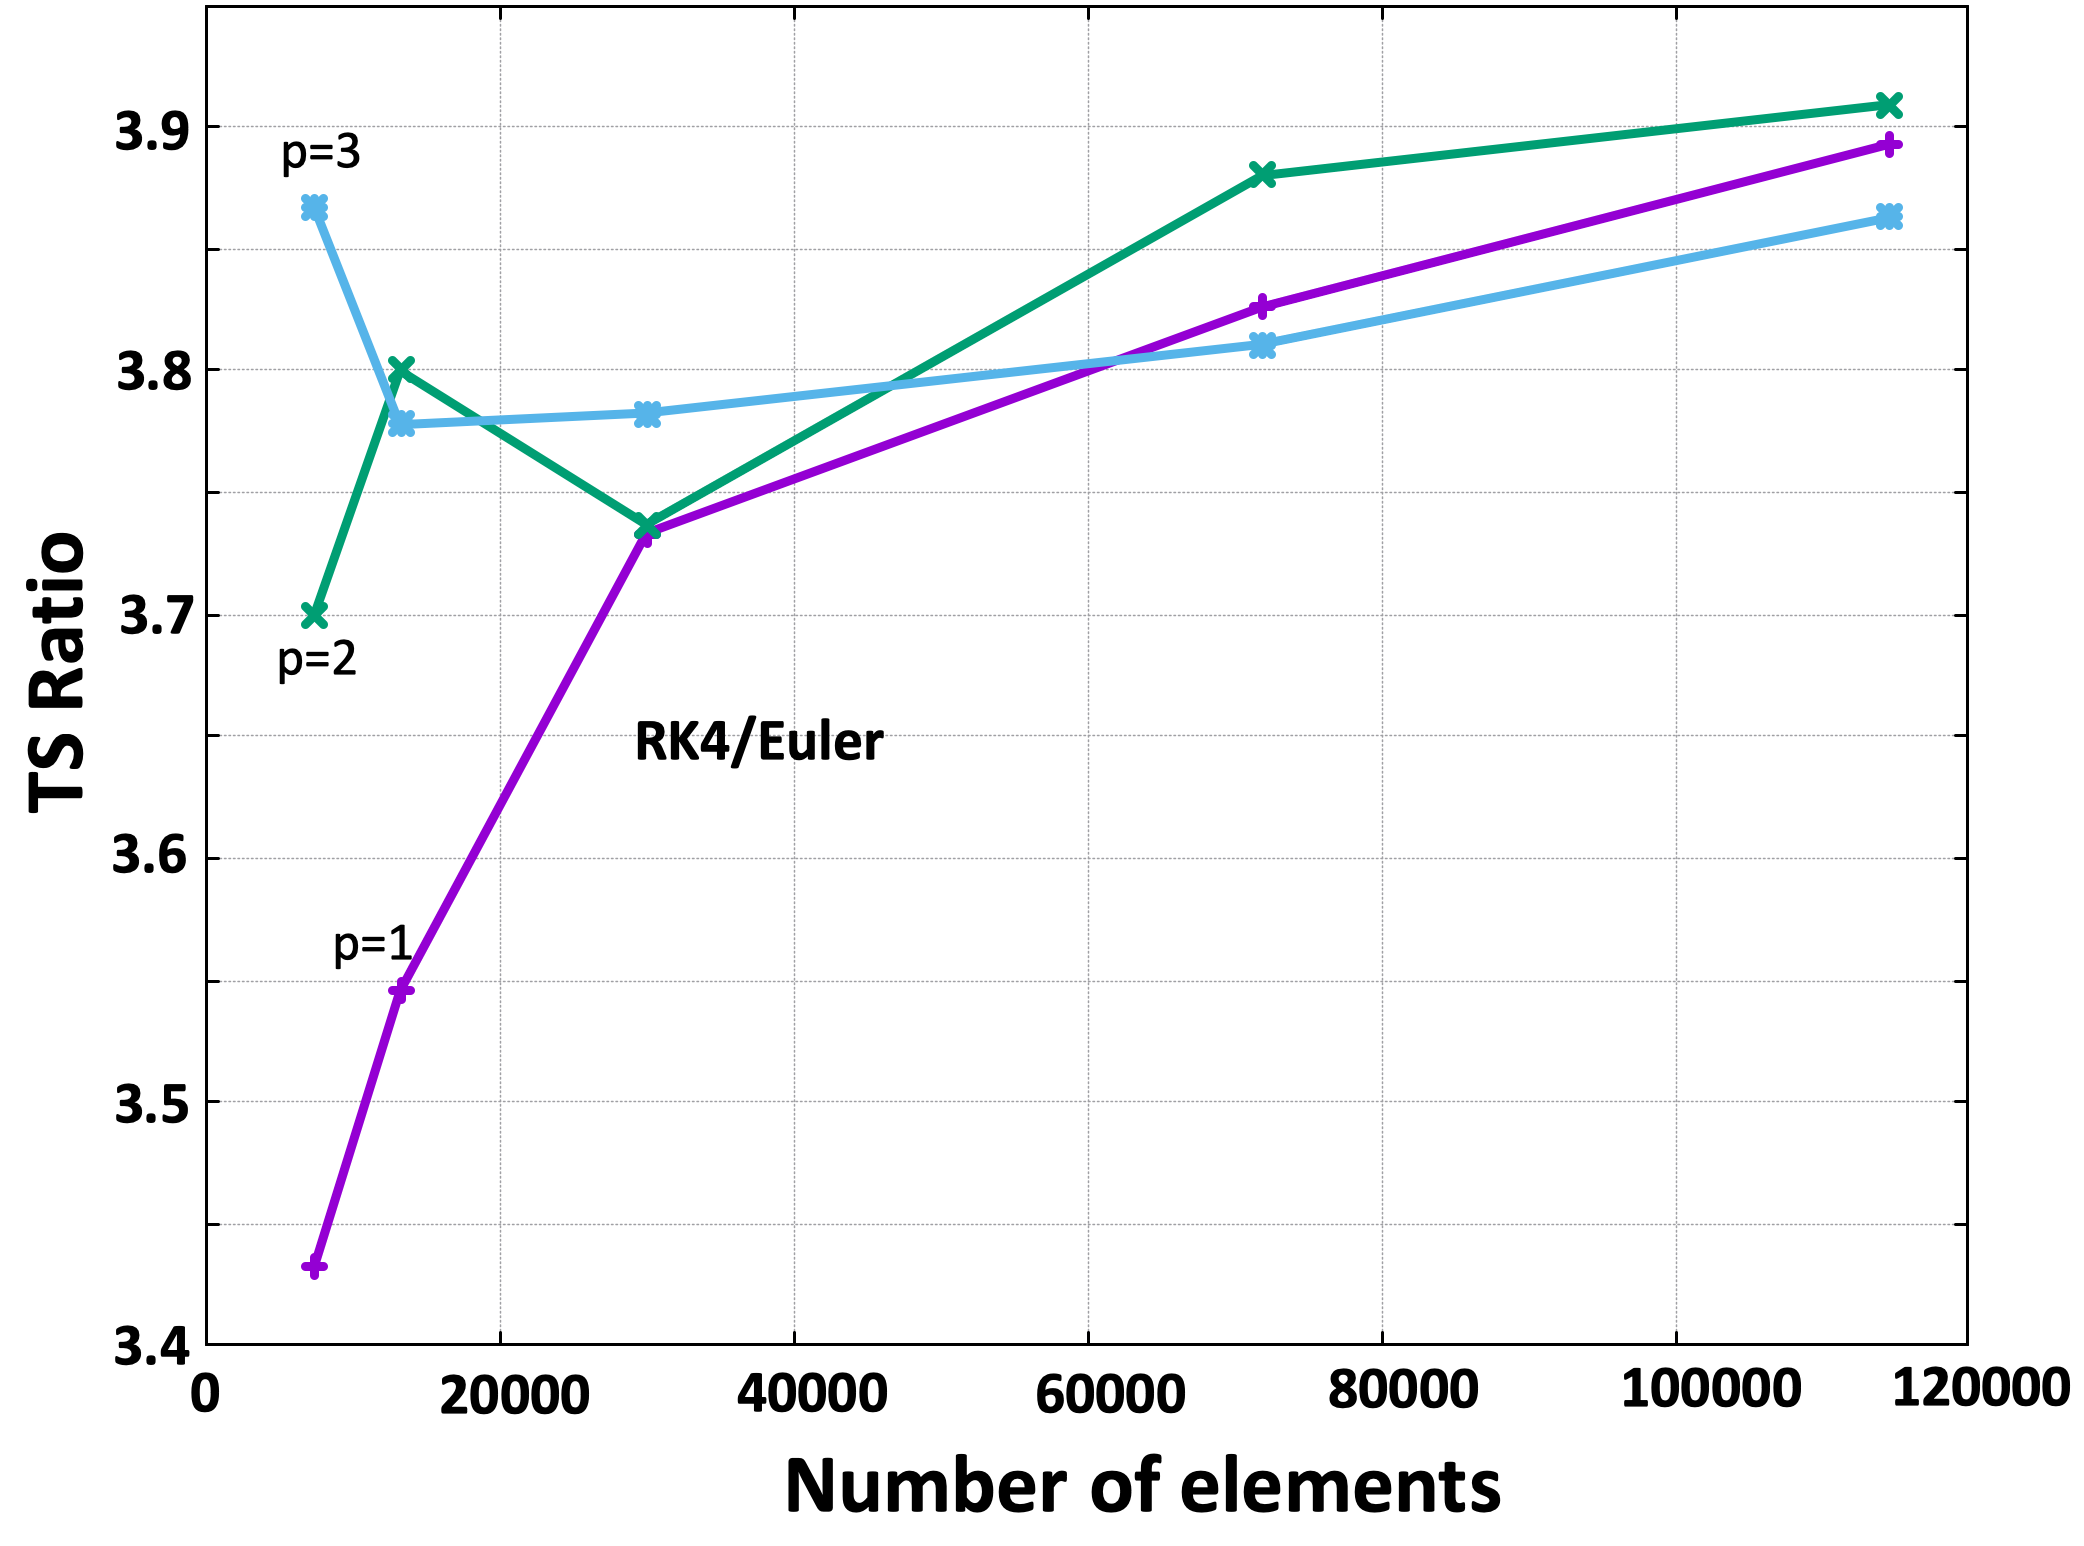
\includegraphics[width=.45\textwidth]{figures/TSRatio.png}
  \begin{tikzpicture}[remember picture, overlay]
    \fill <2> [fill=white, opacity=0.7] (current page.south west) + (0.5,0.5) rectangle (12.5,9);
    \node <2> [inner sep=0pt] at (current page.center) {
      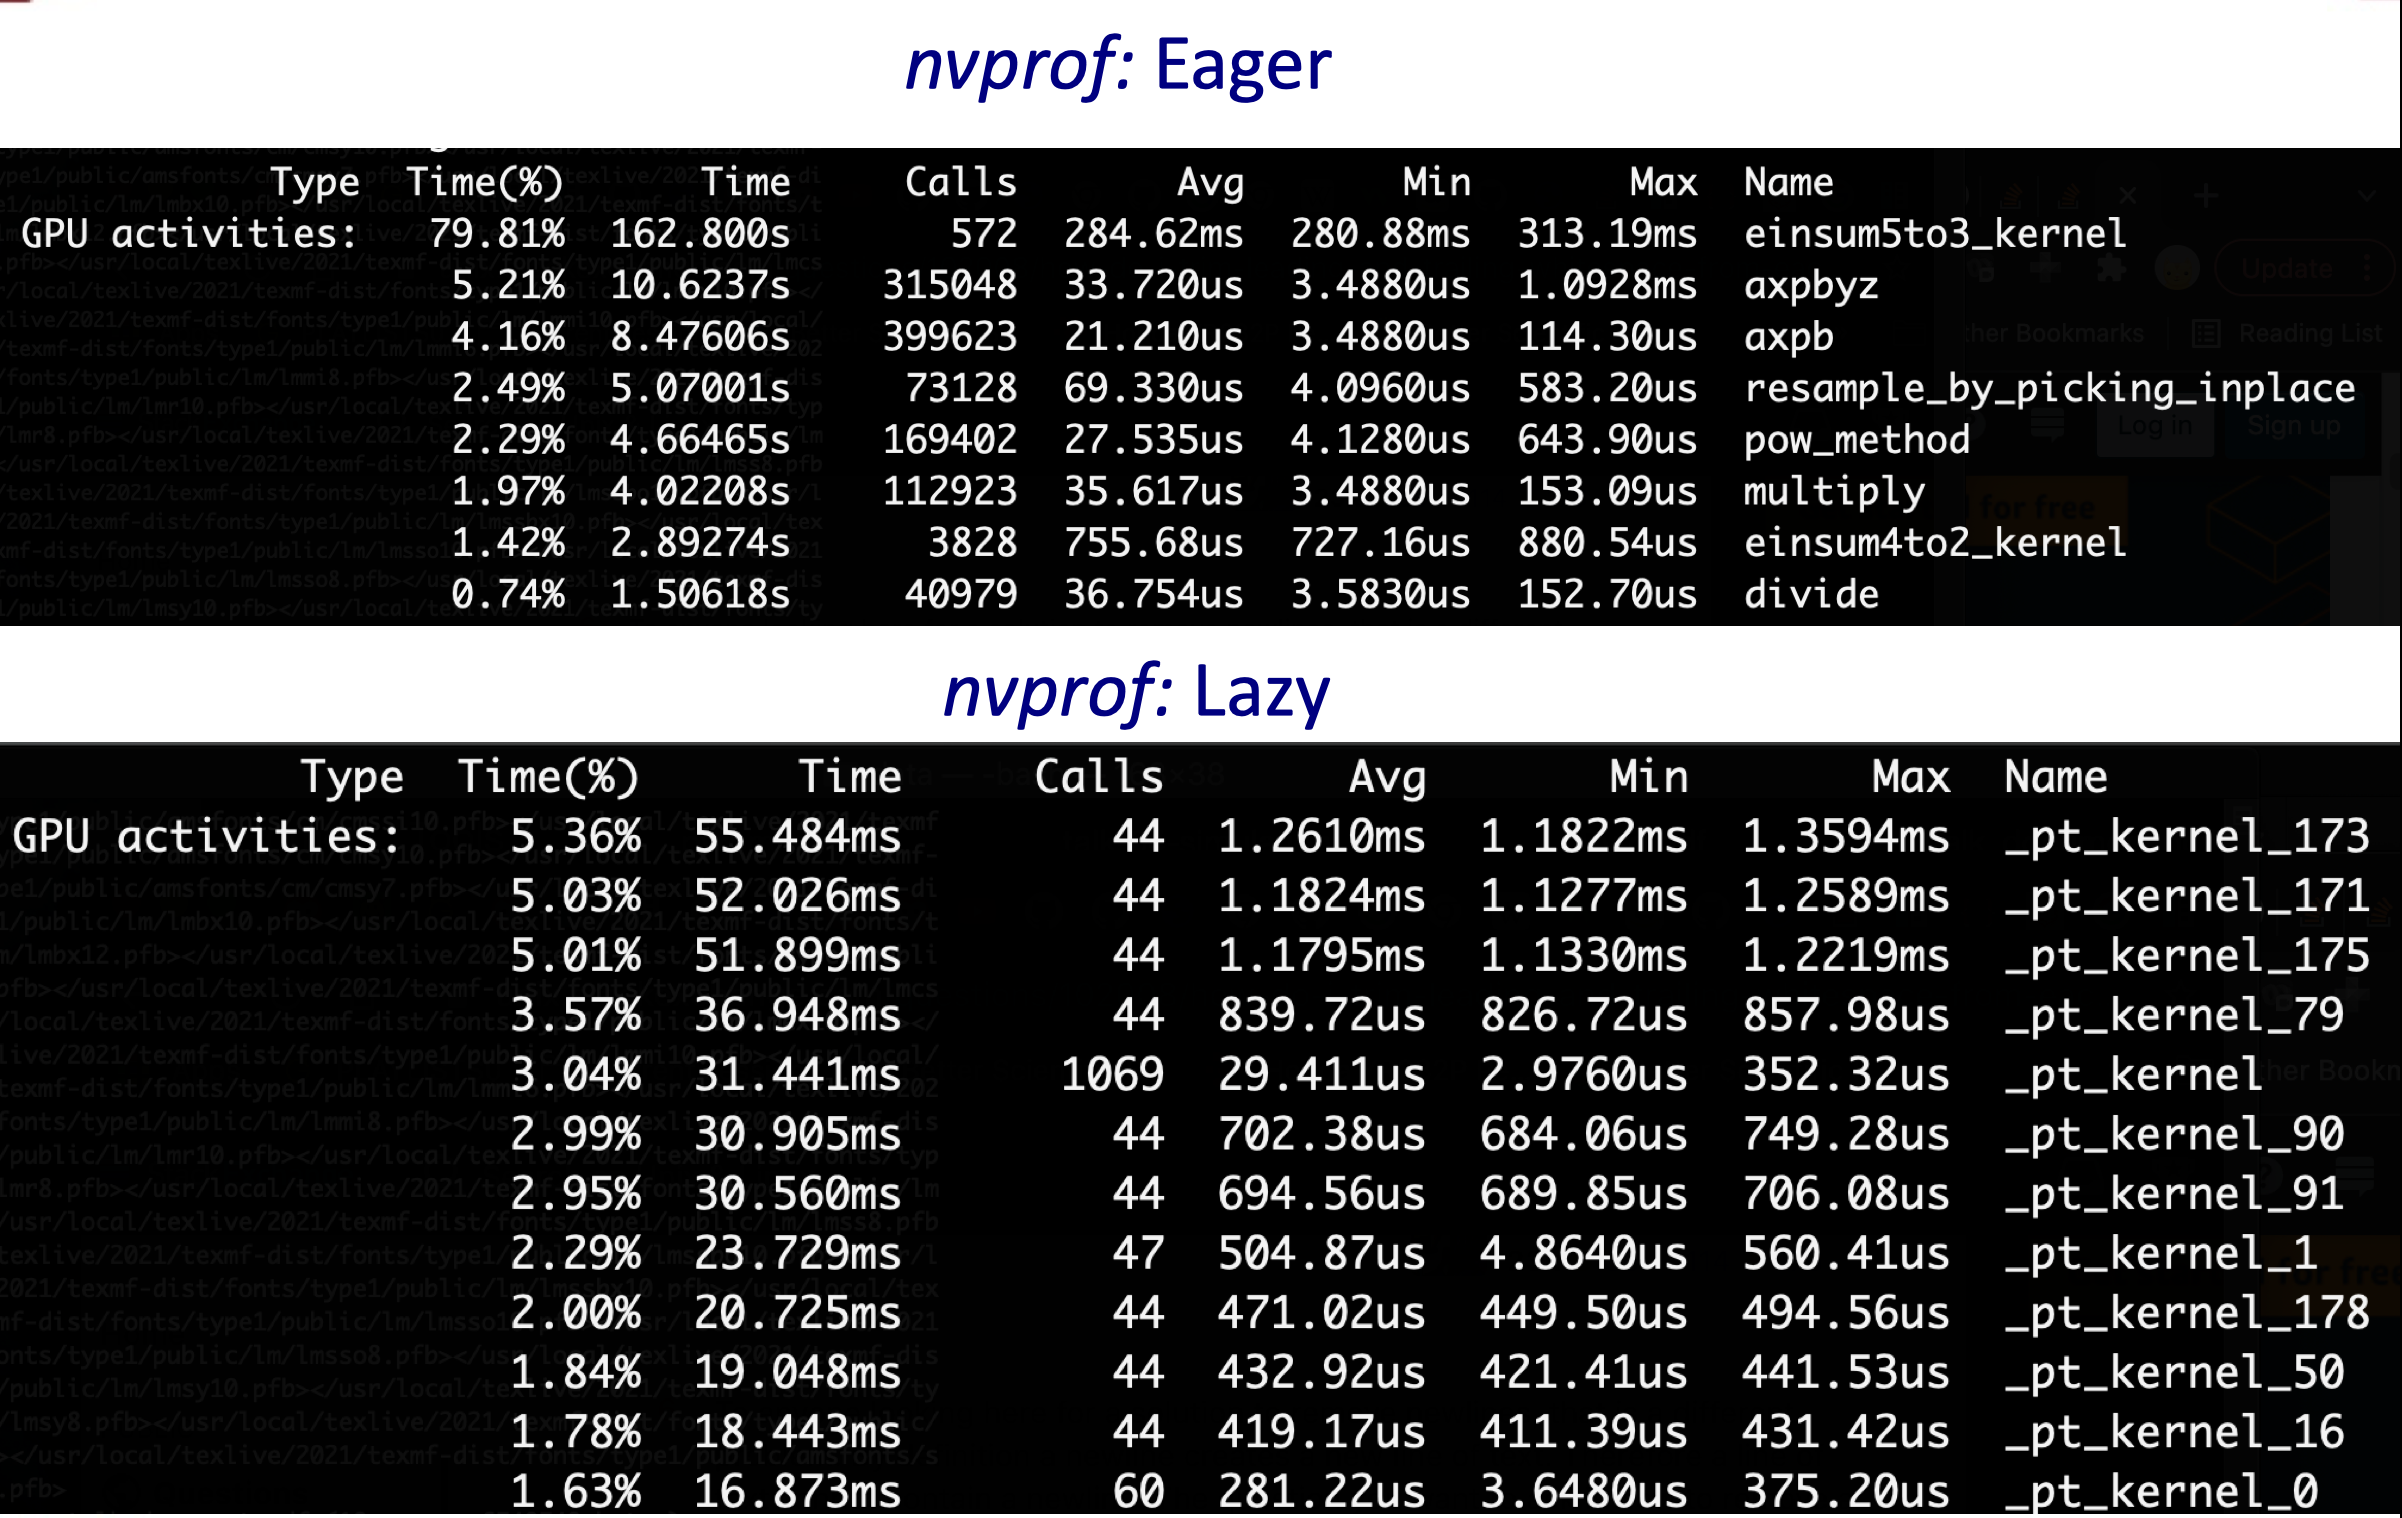
\includegraphics[width=\textwidth]{figures/nvprof_eager_lazy.png}
    };
  \end{tikzpicture}
\end{frame}

\begin{frame}\frametitle{Expected performance?}
\begin{itemize}
\item Flop counting lazy is challenging
\item DG is a local scheme: Expect linear in number of elements
\item Expect linear in number of RHS calls
\end{itemize}
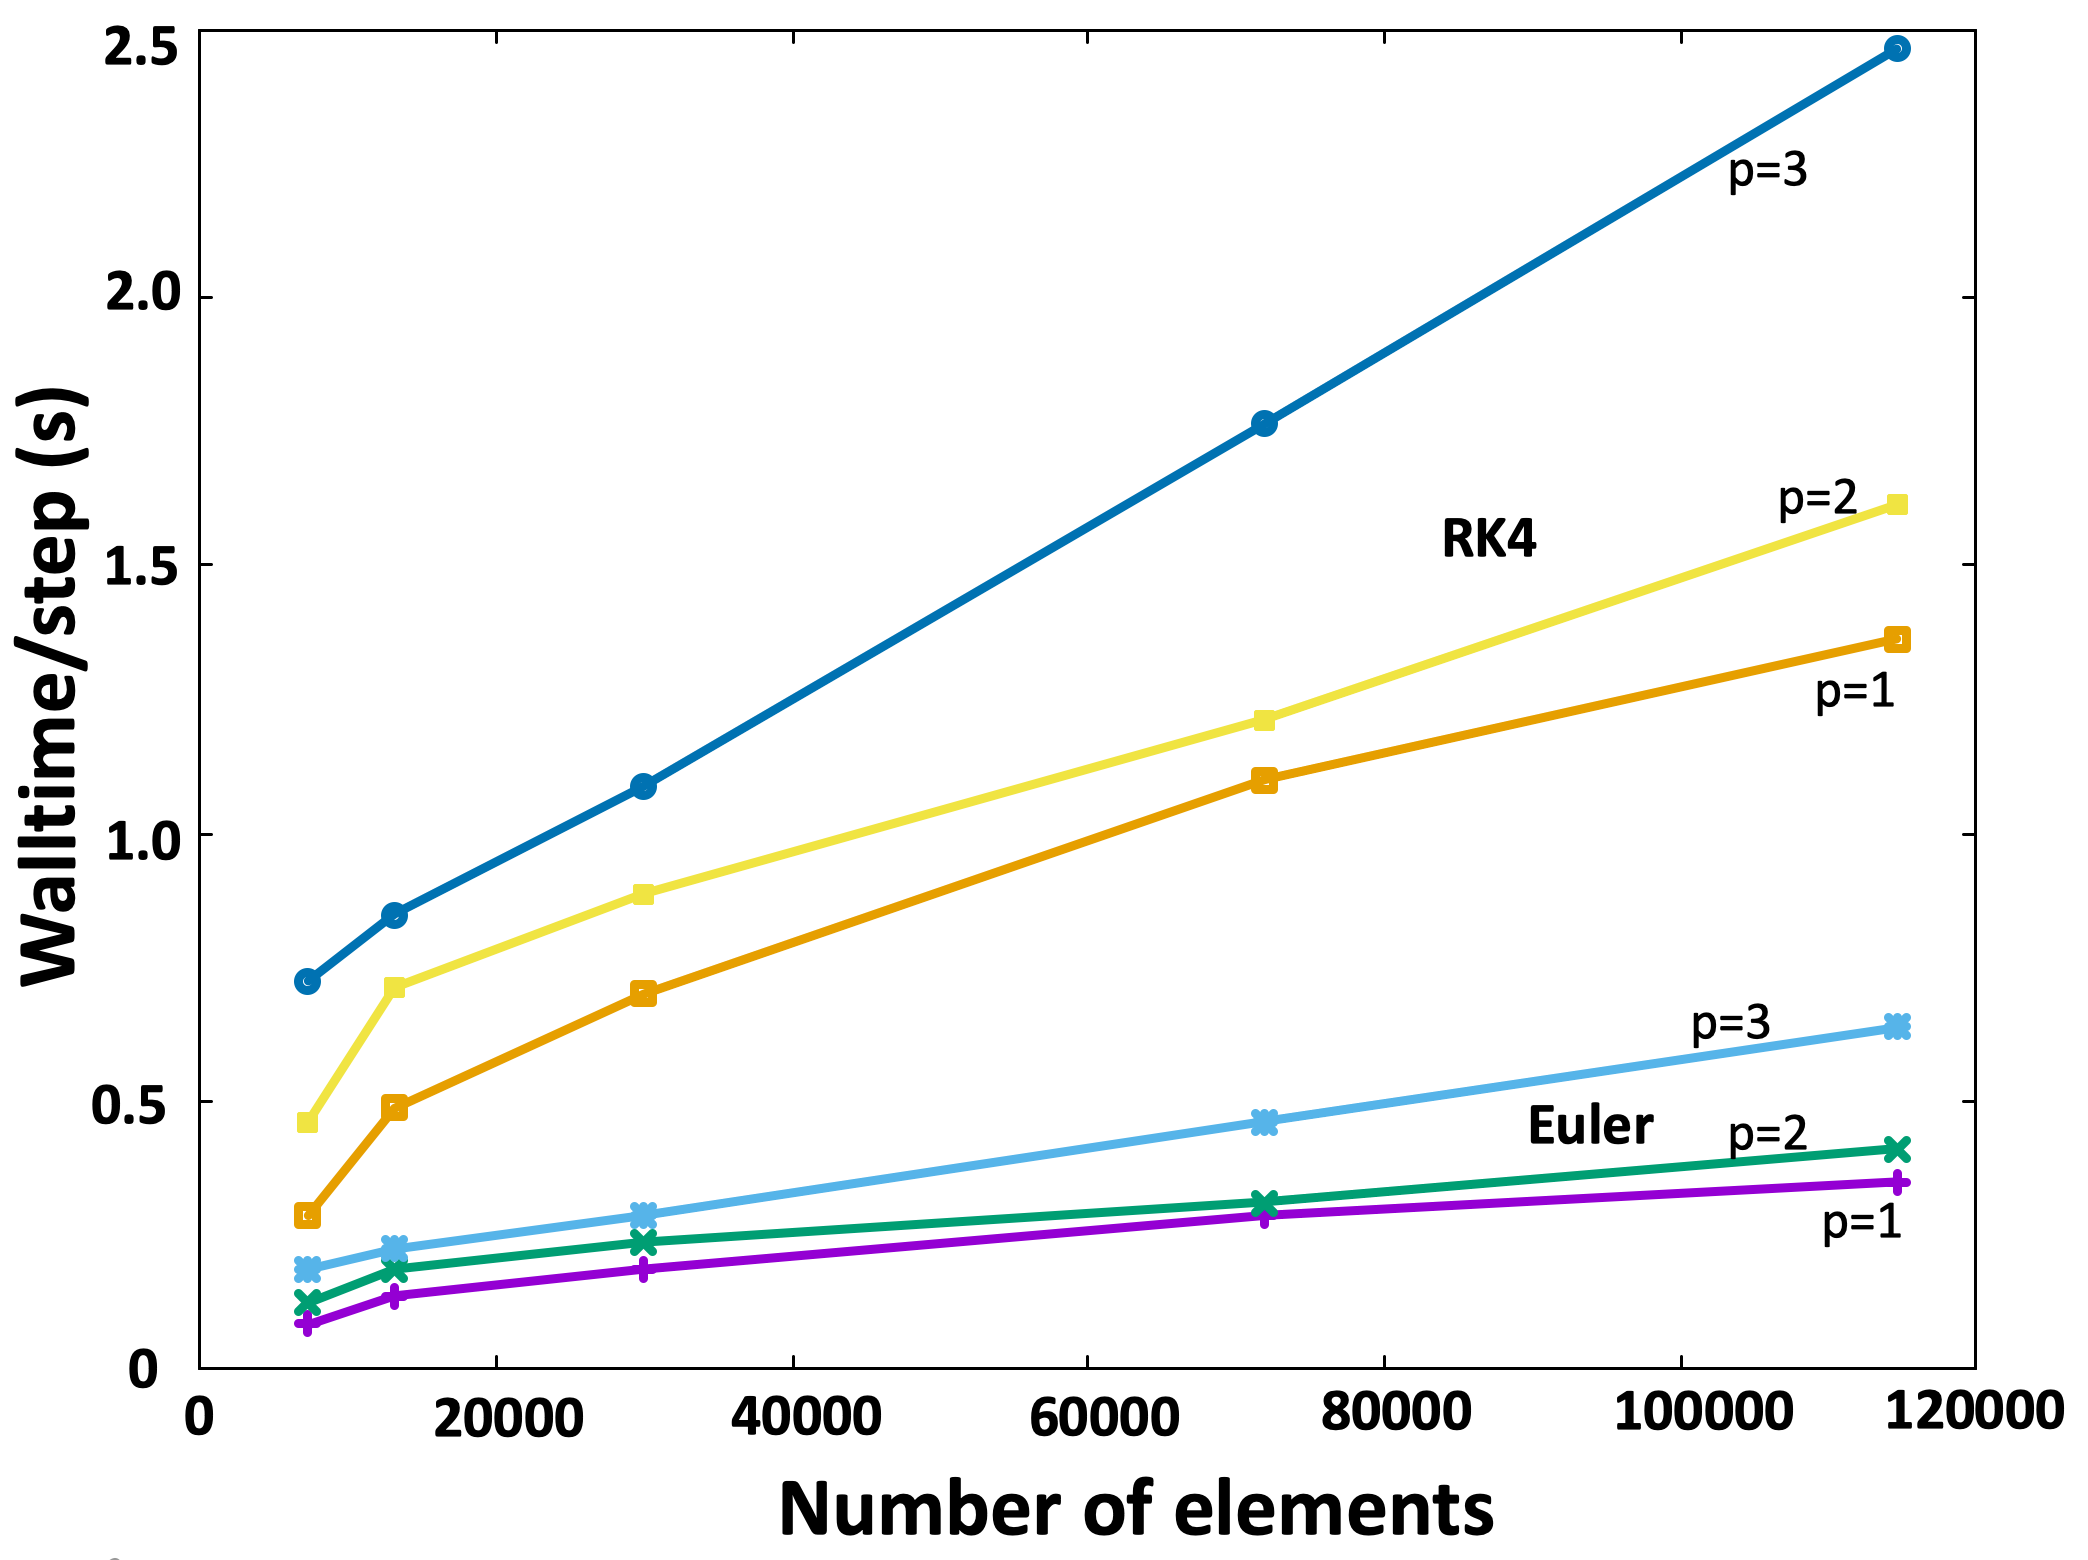
\includegraphics[width=.45\textwidth]{figures/TSCompare.png}
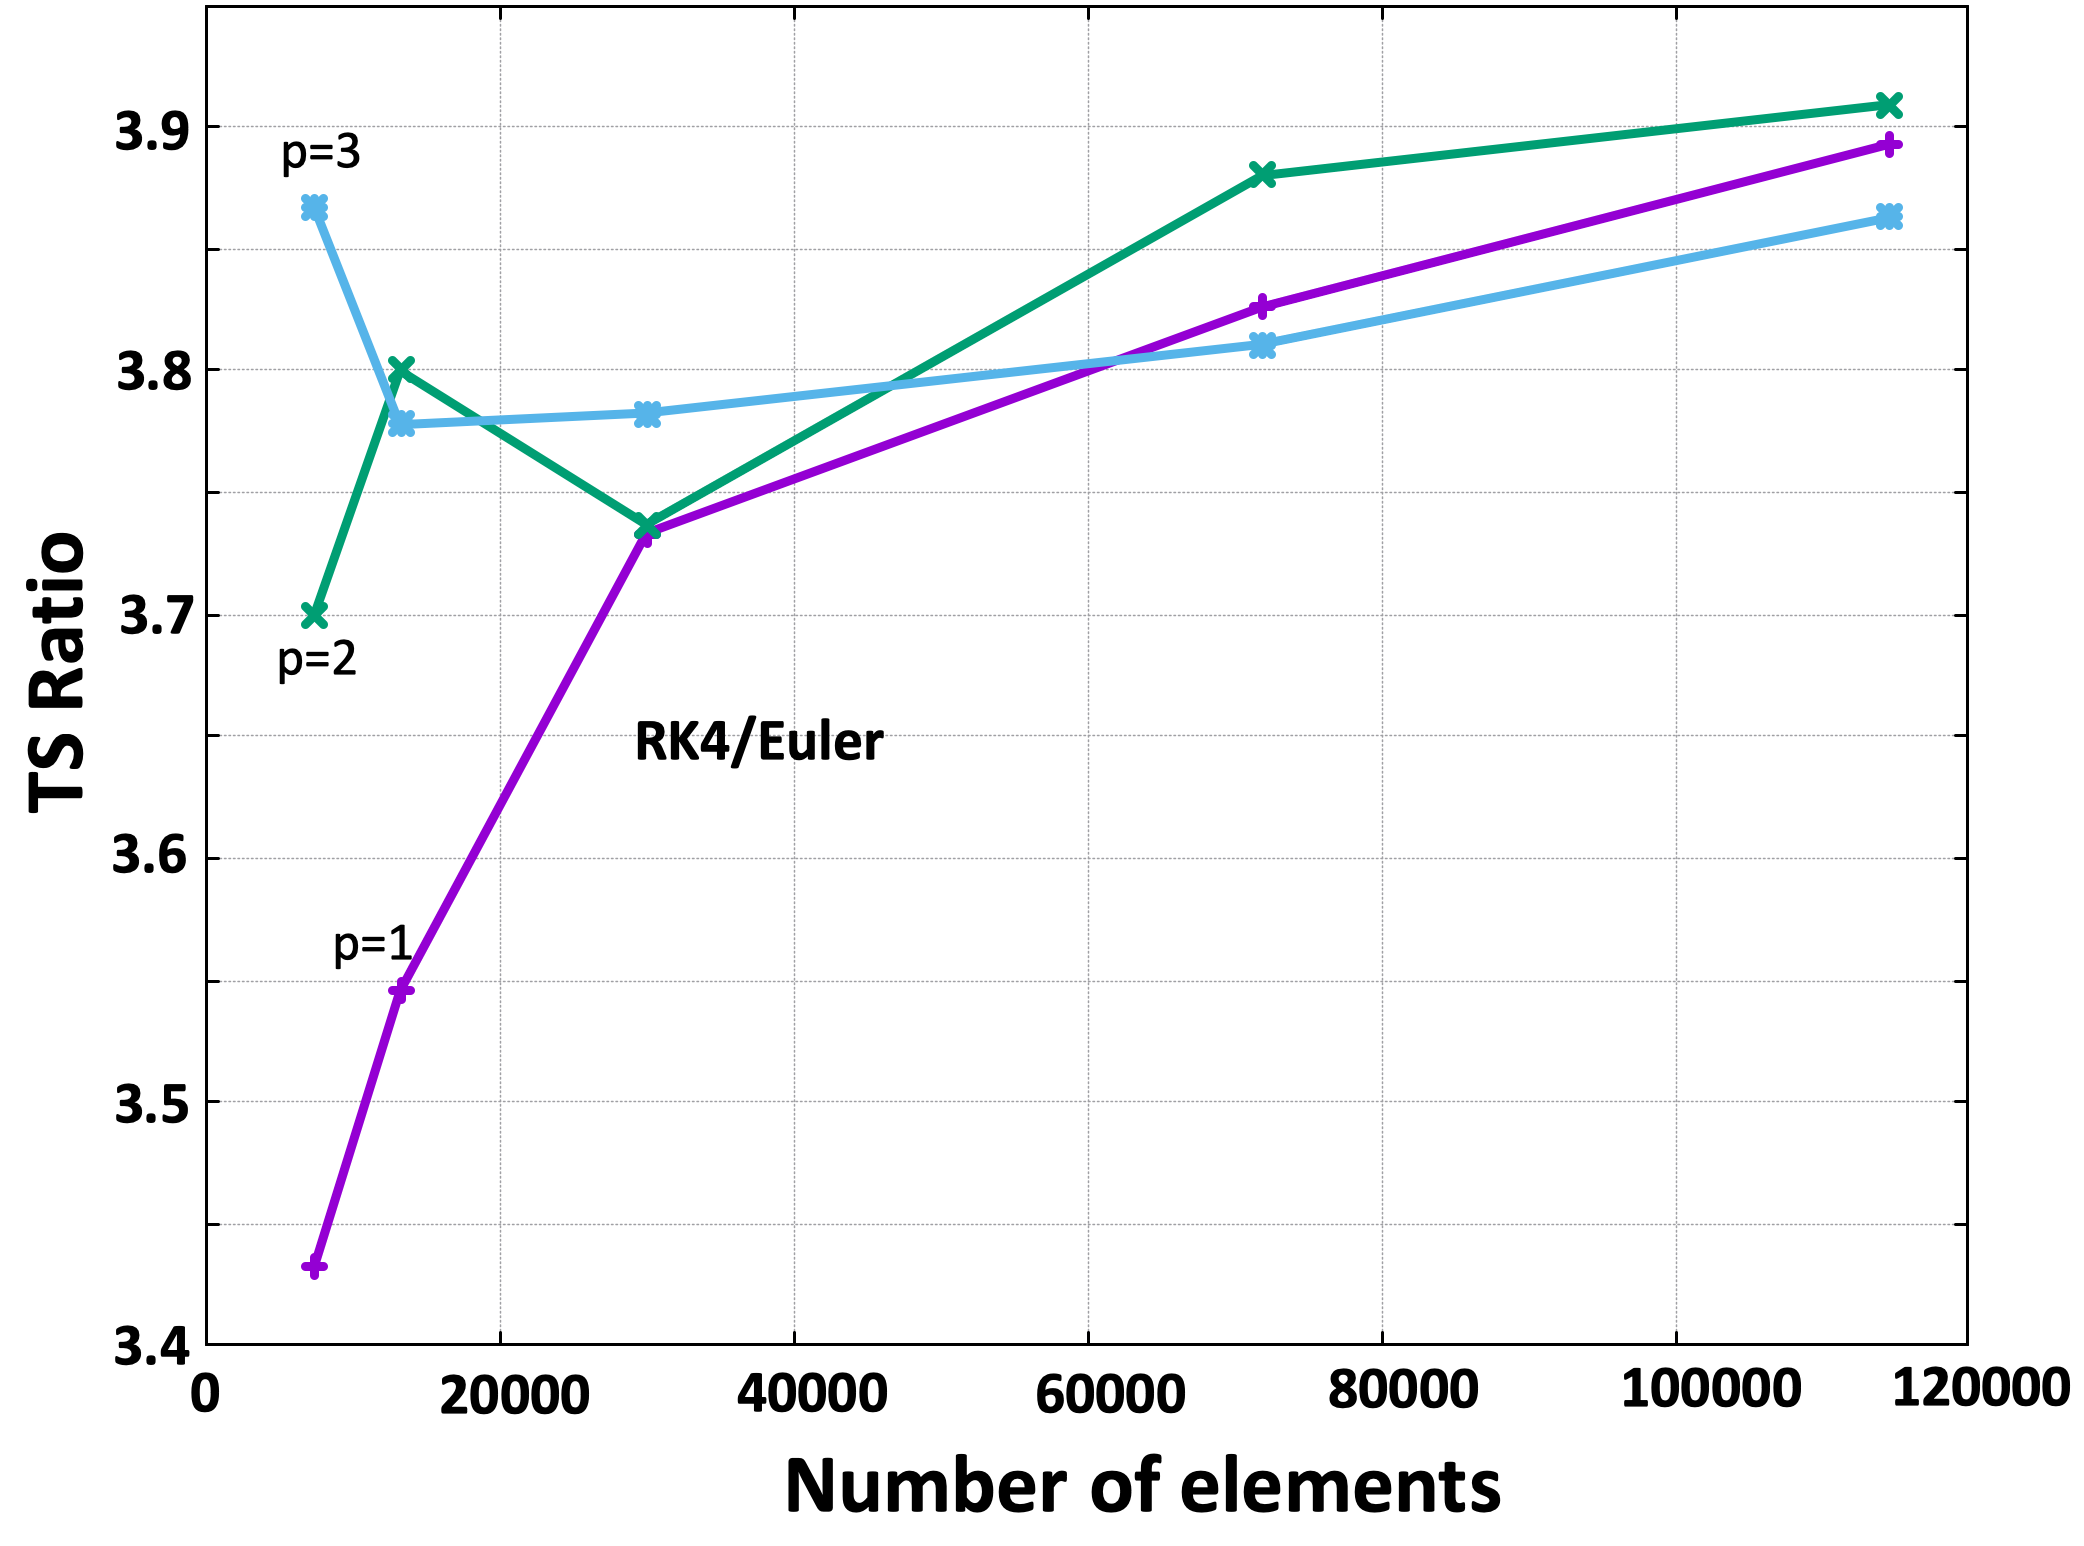
\includegraphics[width=.45\textwidth]{figures/TSRatio.png}
\end{frame}

\begin{frame}\frametitle{Combozzle GPU utilization on Lassen}
\begin{itemize}
\item 100k 3rd order elements, RK4, UIUC mech
\item Using \textit{nvidia-smi}, \textit{nvprof}
\item Illustrating single timestep scale
\begin{minipage}{1.0\textwidth}
 %\begin{figure}
      %\centering
\hspace{-15pt}\includegraphics[width=.45\textwidth]{figures/GPUtilizationEager2.png} 
\includegraphics[width=.45\textwidth]{figures/GPUtilizationLazy2.png}
%    \end{figure}		
  \end{minipage}
\begin{minipage}{1.0\textwidth}
 %\begin{figure}
      %\centering
\hspace{-15pt}\includegraphics[width=.45\textwidth]{figures/GPUMemEager.png} 
\includegraphics[width=.45\textwidth]{figures/GPUMemLazy.png}
%    \end{figure}		
  \end{minipage}
\end{itemize}
  \begin{tikzpicture}[remember picture, overlay]
    \fill <2> [fill=white, opacity=0.7] (current page.south west) + (0.5,0.5) rectangle (12.5,9);
    \node <2> [inner sep=0pt] at (current page.center) {
      \includegraphics[width=\textwidth]{figures/StepperSnippet.png}
    };
  \end{tikzpicture}
\end{frame}


\begin{frame}\frametitle{What's next?}
\begin{center}
\begin{itemize}
\item Lazy evaluation has arrived; eager is right out
\item \mirgecom{} lazy execution is challenging to analyze
\end{itemize}
\end{center}
  \begin{multicols}{2}
    \begin{itemize}
    \item Mixtures \& combustion
    \begin{itemize}
      \item Temperature seeding refactor
      \item Need a better transport model (\pyrometheus)
      \item Lots of exercise (combozzle)
    \end{itemize}
    \end{itemize}
      \columnbreak
      \begin{itemize}   
    \item Performance
      \begin{itemize}
        \item Figure out what the code is doing
        \item Develop a better understanding of the single GPU performance
        \item Get a handle on the expected performance
        \item Continue to closely monitor
      \end{itemize}
    \end{itemize}
  \end{multicols}
  % Far more excited than frightened!
  \begin{center}
    Next for \mirgecom:
    \begin{itemize}
    \item distributed lazy \prj{\tiny}{M.~Diener}
    \item wall modeling and coupling \prj{\tiny}{M.~Smith}
    \end{itemize}
  \end{center}
% \begin{tikzpicture}[remember picture, overlay]
%    \fill <2> [fill=white, opacity=0.7] (current page.south west) + (0.5,0.5) rectangle (12.5,9);
%    \node <2> [inner sep=0pt] at (current page.center) {
%      \includegraphics[width=\textwidth]{figures/nozzle_timing_full.pdf}
%    };
%  \end{tikzpicture}
 \end{frame}

\begin{frame}\frametitle{Performance monitoring: Nozzle}
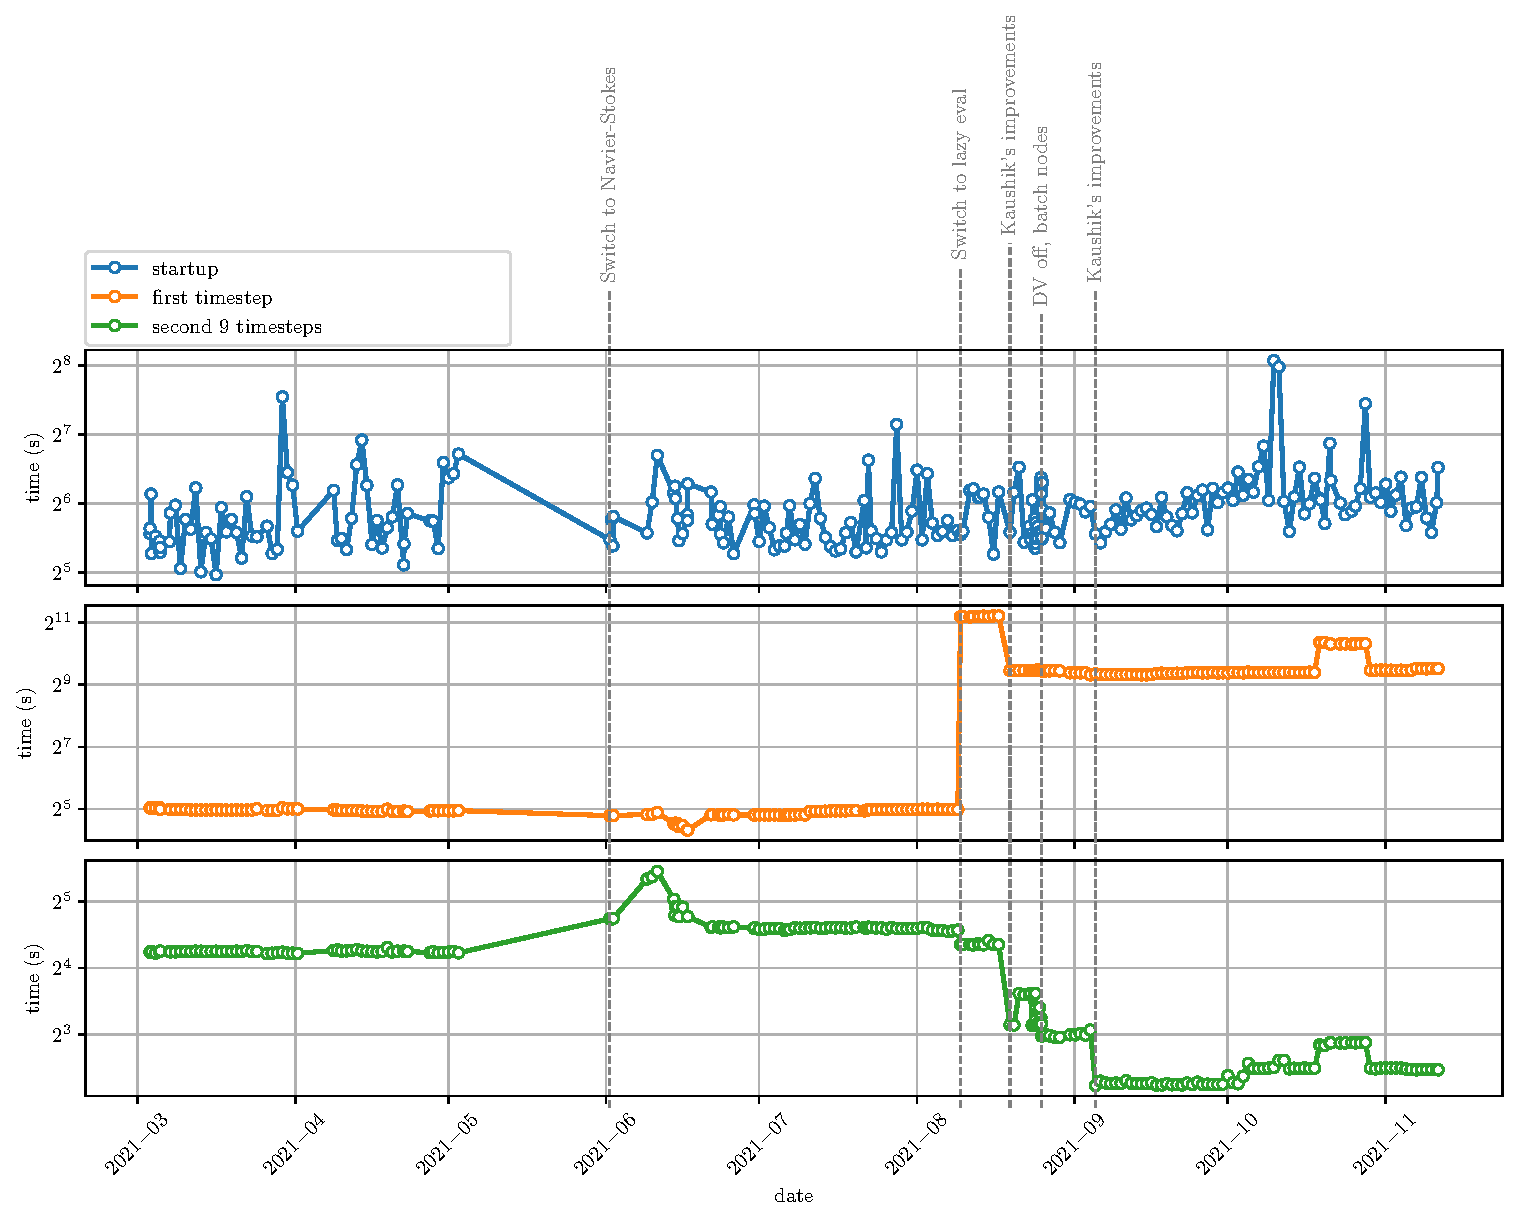
\includegraphics[width=.8\textwidth]{figures/nozzle_20211112.pdf}
\end{frame}

\begin{frame}\frametitle{Performance monitoring: Flame}
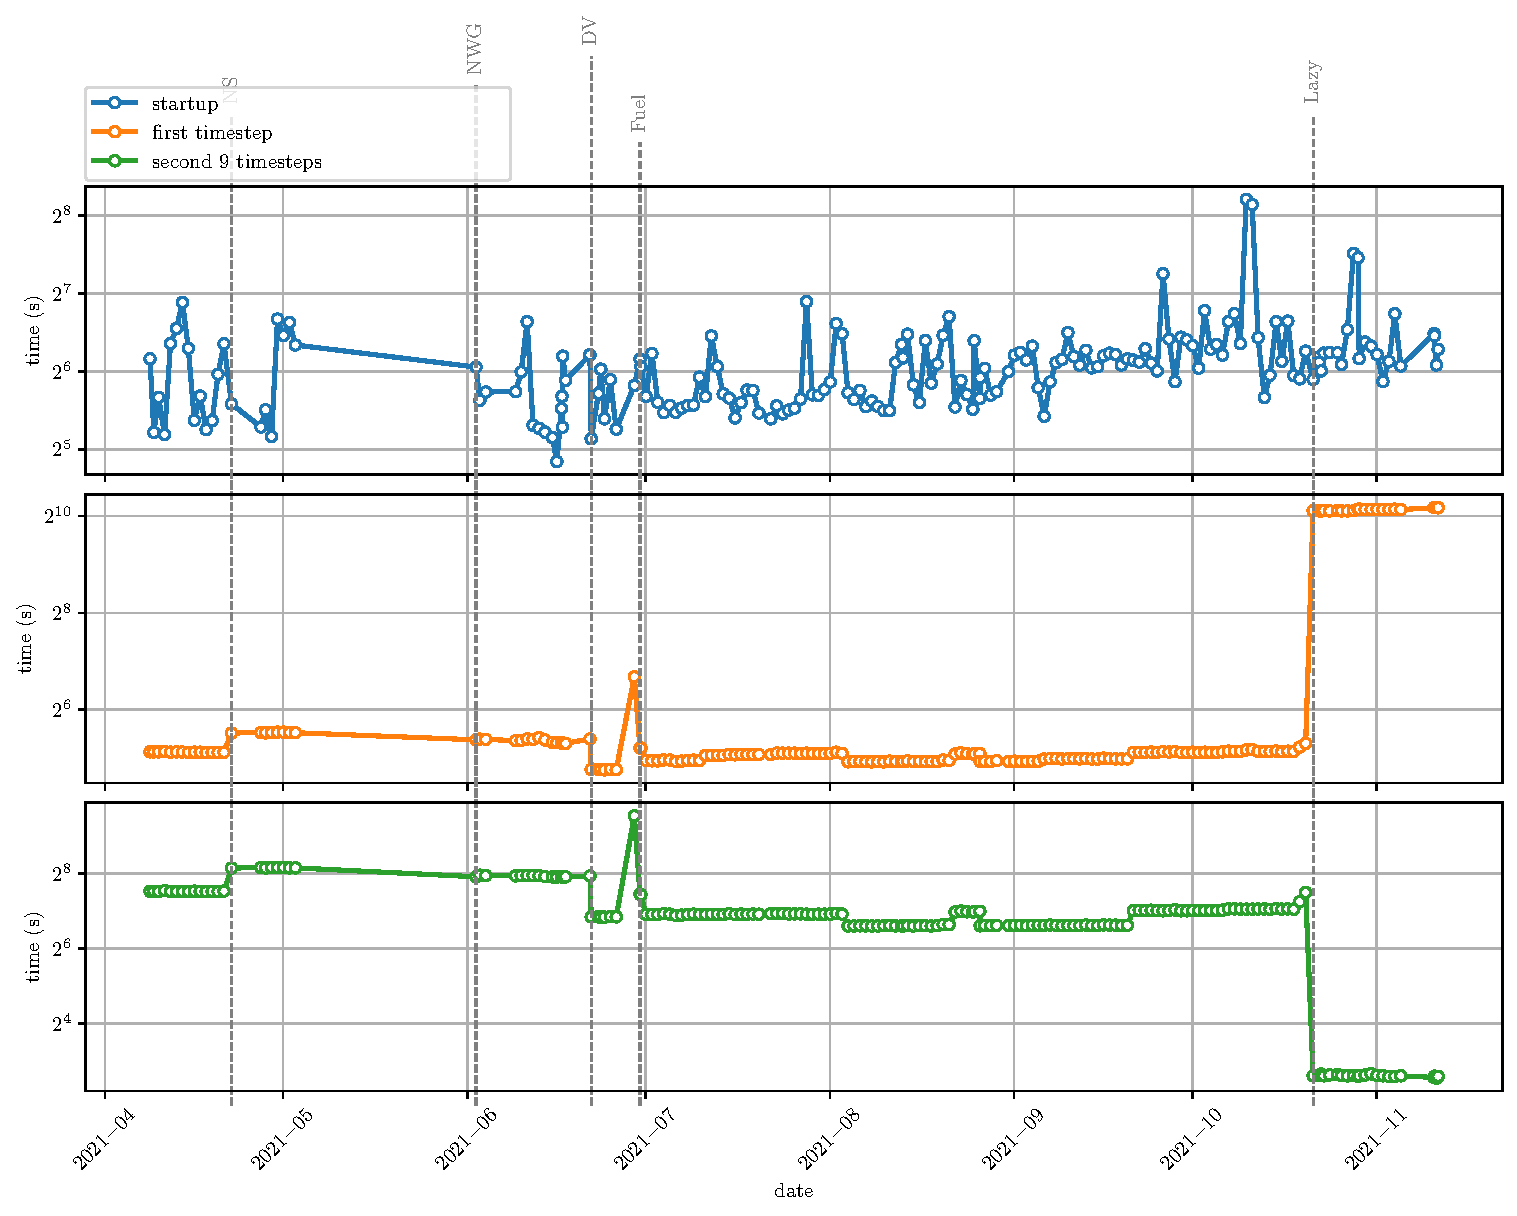
\includegraphics[width=.8\textwidth]{figures/flame_20211112.pdf}
\end{frame}

\begin{frame}\frametitle{Performance monitoring: Isolator}
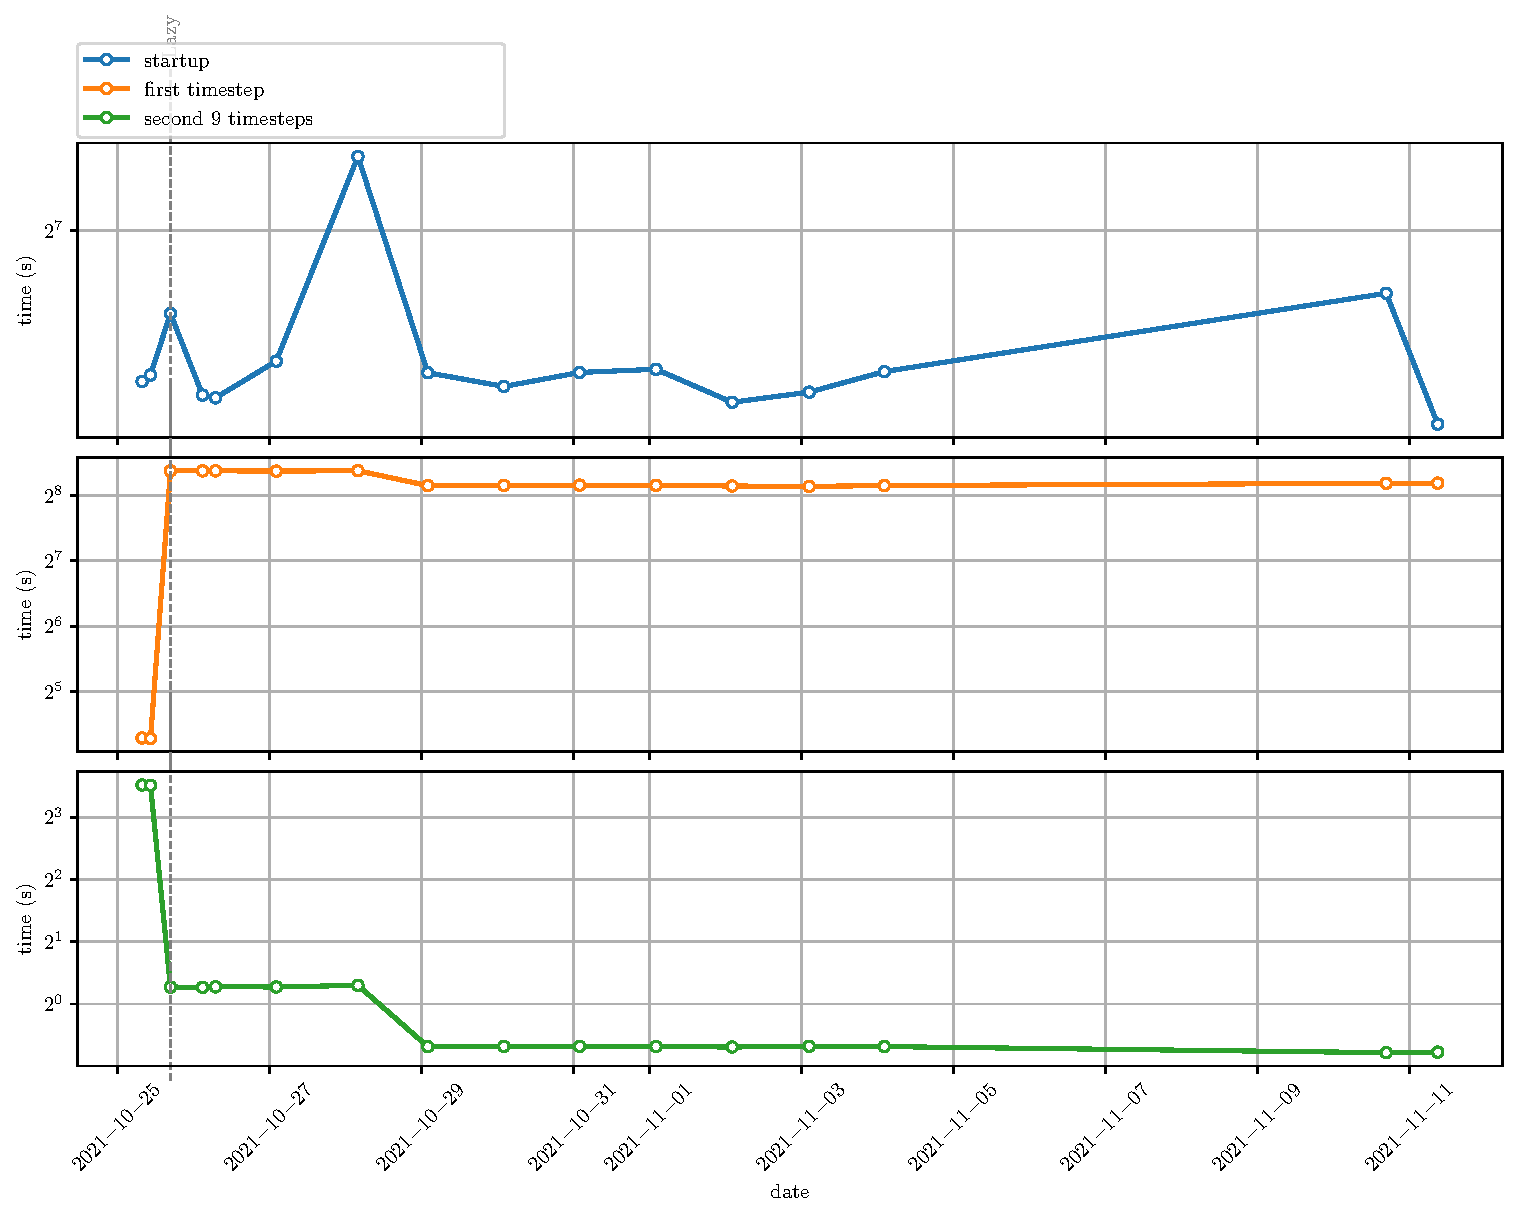
\includegraphics[width=.8\textwidth]{figures/isolator_20211112.pdf}
\end{frame}

\begin{frame}\frametitle{What's next?}
\begin{center}
\begin{itemize}
\item Lazy evaluation has arrived; eager is right out
\item \mirgecom{} lazy execution is challenging to analyze
\end{itemize}
\end{center}
  \begin{multicols}{2}
    \begin{itemize}
    \item Mixtures \& combustion
    \begin{itemize}
      \item Temperature seeding refactor
      \item Need a better transport model (\pyrometheus)
      \item Lots of exercise (combozzle)
    \end{itemize}
    \end{itemize}
      \columnbreak
      \begin{itemize}   
    \item Performance
      \begin{itemize}
        \item Figure out what the code is doing
        \item Develop a better understanding of the single GPU performance
        \item Get a handle on the expected performance
        \item Continue to closely monitor
      \end{itemize}
    \end{itemize}
  \end{multicols}
  % Far more excited than frightened!
  \begin{center}
    Next for \mirgecom:
    \begin{itemize}
    \item distributed lazy \prj{\tiny}{M.~Diener}
    \item wall modeling and coupling \prj{\tiny}{M.~Smith}
    \end{itemize}
  \end{center}
 \begin{tikzpicture}[remember picture, overlay]
    \fill <2> [fill=white, opacity=0.7] (current page.south west) + (0.5,0.5) rectangle (12.5,9);
    \node <2> [inner sep=0pt] at (current page.center) {
      \includegraphics[width=\textwidth]{figures/nozzle_timing_detail.pdf}
    };
  \end{tikzpicture}
 \end{frame}

\begin{frame}\frametitle{What's next?}
\begin{center}
\begin{itemize}
\item Lazy evaluation has arrived; eager is right out
\item \mirgecom{} lazy execution is challenging to analyze
\end{itemize}
\end{center}
  \begin{multicols}{2}
    \begin{itemize}
    \item Mixtures \& combustion
    \begin{itemize}
      \item Temperature seeding refactor
      \item Need a better transport model (\pyrometheus)
      \item Lots of exercise (combozzle)
    \end{itemize}
    \end{itemize}
      \columnbreak
      \begin{itemize}   
    \item Performance
      \begin{itemize}
        \item Figure out what the code is doing
        \item Develop a better understanding of the single GPU performance
        \item Get a handle on the expected performance
        \item Continue to closely monitor
      \end{itemize}
    \end{itemize}
  \end{multicols}
  % Far more excited than frightened!
  \begin{center}
    Next for \mirgecom:
    \begin{itemize}
    \item distributed lazy \prj{\tiny}{M.~Diener}
    \item wall modeling and coupling \prj{\tiny}{M.~Smith}
    \end{itemize}
  \end{center}
 \end{frame}

%\begin{frame}\frametitle{Daily ASC platform tests}
%  %    \vspace{0pt}
%  \setlength{\columnsep}{-7.0cm}
%  \begin{multicols}{2}
%    \begin{minipage}{.2\textwidth}
%      \vspace{1cm}
%      \hspace{-2cm}
%    \begin{itemize}
%    \item Lassen GPUs%\hspace{-2cm}%
%    \item 1(+) times daily cron
%    \item Exercises nozzle, 1dflame
%    \end{itemize}
%    \end{minipage}
%    \columnbreak
%    \hspace{-80pt}
%    \begin{figure}[htpb]
%      \includegraphics[width=.8\textwidth]{figures/nozzle_timing_full.pdf}
%    \end{figure}		
%  \end{multicols}
%  \vspace{0pt}
%  \begin{tikzpicture}[remember picture, overlay]
%    \fill <2> [fill=white, opacity=0.8] (current page.south west) + (0.5,0.5) rectangle (12.5,9);
%    \node <2> [inner sep=0pt] at (current page.center) {
%      \includegraphics[width=\textwidth]{figures/nozzle_timing_detail.pdf}
%    };
%  \end{tikzpicture}
  % make a grid:
  % \tikz[overlay, remember picture, help lines]{
  %   \foreach \x in {0,...,12} \path (current page.south west) +(\x,9.25) node {\small$\x$};
  %   \foreach \y in {0,...,9} \path (current page.south west) +(12.5,\y) node {\small$\y$};
  %   \foreach \x in {0,0.5,...,12.5} \draw (current page.south west) ++(\x,0) -- +(0,9.6);
  %   \foreach \y in {0,0.5,...,9.5} \draw (current page.south west) ++(0,\y) -- +(12.8,0);
  % }
  %
%\end{frame}

%\begin{frame}\frametitle{MIRGE-Com development environment}
%  \begin{itemize}
%  \item development process/env
%  \item user/developer support
%  \item production support (y1-production)
%  \item testing: unit, integrated, verification/regression, production, nightly timings
%  \end{itemize}
%\end{frame}


%\begin{frame}\frametitle{Production timing history}
%  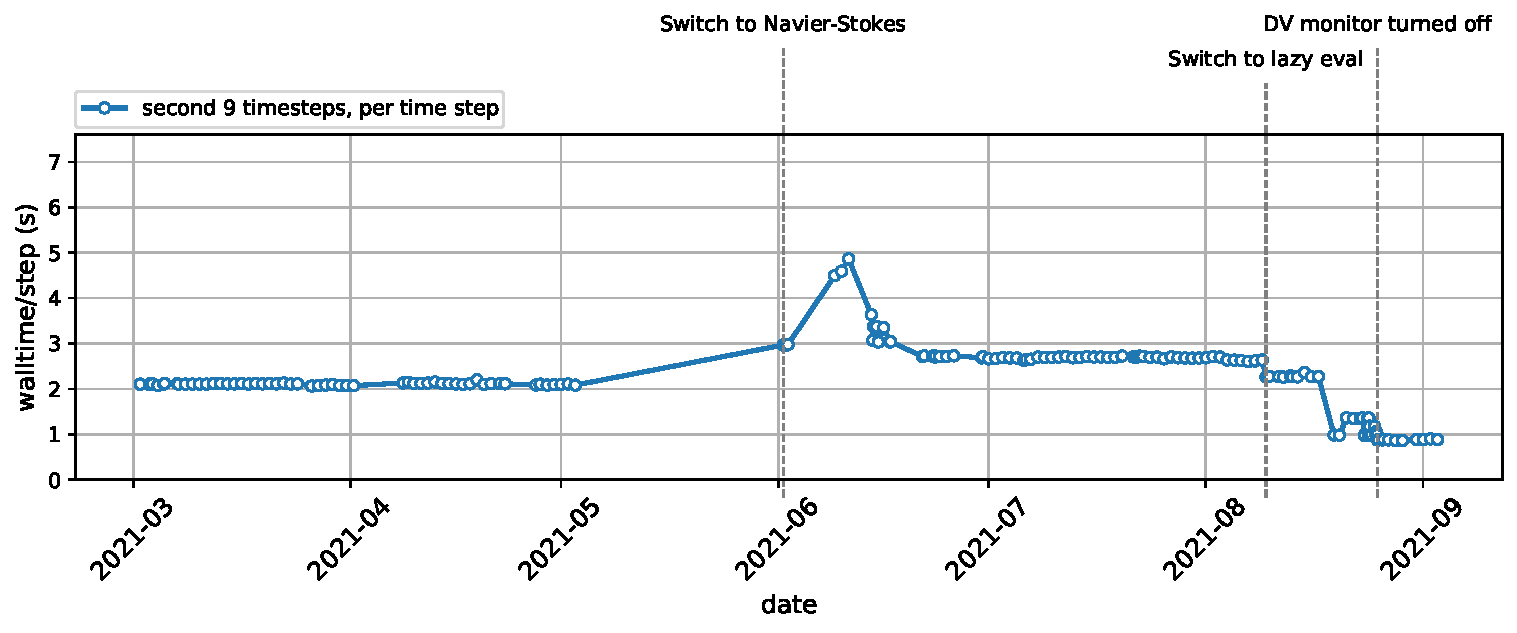
\includegraphics[width=\textwidth]{figures/nozzle_timing.pdf} 
%\end{frame}

%\begin{frame}\frametitle{Conclusion and wrap-up}
%\end{frame}




%======================================================================
%\begin{frame}\frametitle{MIRGECom status and developments}
%  \begin{center}
%    Outline
%  \end{center}
%  \begin{itemize}
%  % MIRGE (Com) and how it is constructed, how it comes together
%  \item High-level architecture
%    
%  \item Navier-Stokes w/mixtures \& wall cartoon
%    \begin{itemize}
%    \item highlight current \& to come (Wyatt - shock capt, MattS - wall model, Esteban - thermochem kinetics)
%    \item show example code expressions for NS
%    % How prometheus connects
%    \item show \pyrometheus integration plan (and how is currently implemented)
%    \end{itemize}
%  \item MIRGE-Euler example(s):
%    \begin{itemize}
%    \item Building a driver
%    \item Brief about I/O \& analysis (maybe in arch overview?)
%    \item Autoignition example 
%    \item Allude to MikeA's Y0 sim
%    \end{itemize}
%  \end{itemize}
%\end{frame}
%======================================================================

%\begin{frame}\frametitle{Core packages}
%\begin{itemize}
%  \item Loo.py (\href{https://github.com/inducer/loopy}{(\textcolor{blue}{https://github.com/inducer/loopy})})
%  \begin{itemize}
%    \item Code generator and transform tool
%    \item IR in MIRGE
%    \item Element-wise computational kernels
%  \end{itemize}
%  \item Meshmode (\href{https://github.com/inducer/meshmode}{(\textcolor{blue}{https://github.com/inducer/meshmode})})
%  \begin{itemize}
%    \item Uns., high-order, discont. piecewise polynomial discretizations 
%    \item DG building blocks (see \texttt{examples/simple-dg.py}).
%  \end{itemize}
%  \item \textit{Grudge} - 1/2/3D DG based on \textit{meshmode} (\href{https://github.com/inducer/grudge}{(\textcolor{blue}{https://github.com/inducer/grudge})})
%  \begin{itemize}
%    \item Multiple \textit{meshmode} discretizations
%    \item Methods and operations - math, projections, norms and reductions
%  \end{itemize}
%\end{itemize}
%\end{frame}

%\begin{frame}\frametitle{Development team}
%\begin{multicols}{2}
%\begin{itemize}
%\item Mike Anderson - predictions, modeling
%\item Mike Campbell - sim/solver development
%\columnbreak
%\item Matthias Diener - environment, platforms, performance
%\item Matt Smith  - sim/solver development, grids/geometry
%\end{itemize}
%\end{multicols}
%\end{frame}

%\begin{frame}\frametitle{Target problem}
%  \begin{itemize}
%  \item Domain cartoon
%    % MIRGE (Com) and how it is constructed, how it comes together
%  \item Navier-Stokes w/mixtures \& chemical sources for fluid \& wall cartoon
%  \item Wall and viscous fluxes - Matt Smith heat eqn solver
%  \item Inviscid part - expressions for fluxes, implementation
%  \item Chemistry, \pyrometheus - Esteban
%    \begin{itemize}
%    \item architecture plug here \& generator use to generate python
%    \item expression for sources, implementation
%    \end{itemize}
%  \item Shock-capturing - Wyatt Hagen
%  \end{itemize}
%\end{frame}

%\begin{frame}\frametitle{User experience}
%  \begin{itemize}
%  \item Problem setup
%    \begin{itemize}
%    \item Grid - generate or read in (M. Smith hook)
%    \item Building a driver
%    \item Brief about I/O \& analysis (maybe in arch overview?)
%    \end{itemize}
%  \item Example drivers
%    \begin{itemize}
%    \item Isentropic vortex verif
%    \item Autoignition example 
%    \item Allude to MikeA's Y0 sim
%    \end{itemize}
%  \end{itemize}
%\end{frame}

%\begin{frame}\frametitle{High-level architecture}
%\end{frame}

%\begin{frame}\frametitle{Getting started with \textit{MIRGE-Com}}
%\begin{multicols}{2}
%\begin{itemize}
%  \item \textit{Emirge} - \textit{MIRGE-Com} installation tool
%  \begin{itemize}
%    \item > git clone https://github.com/illinois-ceesd/emirge
%    \item > install.sh
%    \item > source config/activate\_env.sh
%  \end{itemize}
%  \item \textit{MIRGE-Com} documentation
%  \begin{itemize}
%    \item > conda install sphinx
%    \item > cd mirgecom/doc \&\& make html
%  \end{itemize}
%\end{itemize}
%%\hspace{.8in}
%%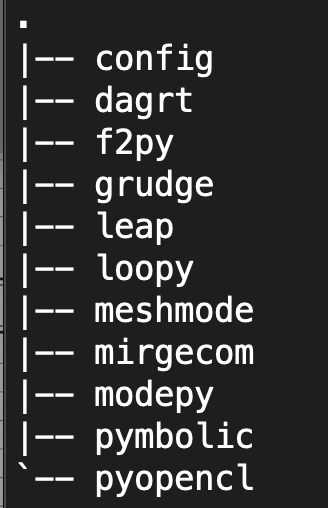
\includegraphics[width=.2\textwidth]{figures/mtc/emirge_dirs.png}
%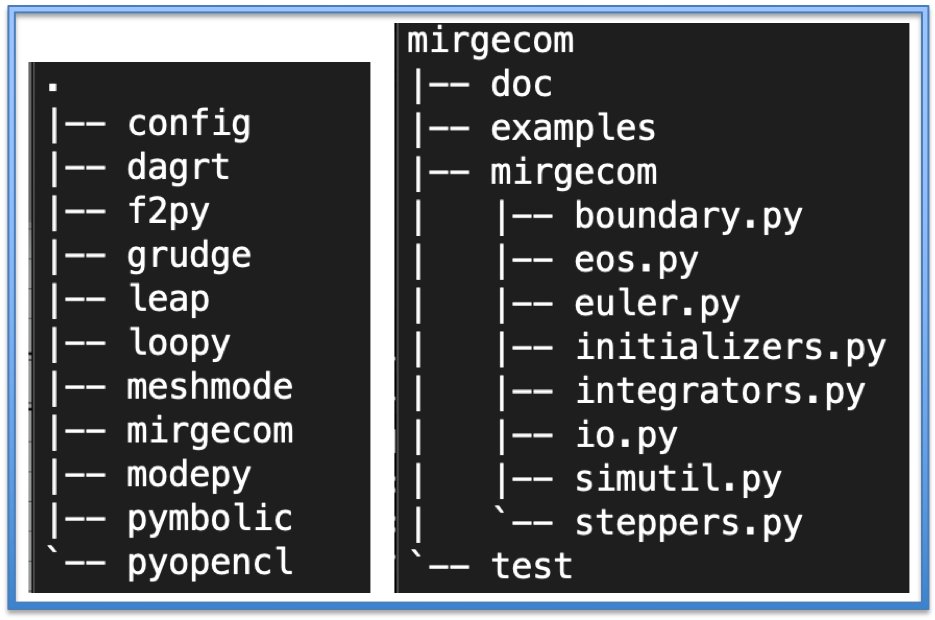
\includegraphics[width=.5\textwidth]{figures/mtc/dir_trees.png}
%\end{multicols}
%\begin{center}
%\href{https://github.com/illinois-ceesd/emirge}{(\textcolor{blue}{https://github.com/illinois-ceesd/emirge})}
%\href{https://mirgecom.readthedocs.io/en/latest/}{(\textcolor{blue}{https://mirgecom.readthedocs.io/en/latest/})}
%\end{center}
%\end{frame}


%\begin{frame}\frametitle{DG Support - Sub-discretizations (dd)}
%  \begin{multicols}{2}
%    \begin{itemize}
%    \item Projections between sub-discretizations: ``vol'' $\rightarrow$ ``int\_faces''
%    \end{itemize}
%    \lstinputlisting[style=kkcodestyle, basicstyle=\scriptsize, language=Python]{figures/mtc/project_sample.py}
%    \columnbreak
%    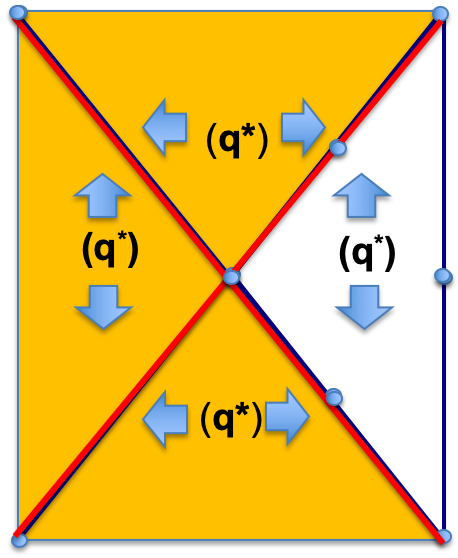
\includegraphics[width=.5\textwidth]{figures/mtc/grid_cartoon_6.png}
%  \end{multicols}
%\end{frame}

%\begin{frame}\frametitle{DG Support - Sub-discretizations (dd)}
%  \begin{multicols}{2}
%    \begin{itemize}
%    \item Unit normal to sub-discretizations
%    \end{itemize}
%    \lstinputlisting[style=kkcodestyle, basicstyle=\scriptsize, language=Python]{figures/mtc/normal_sample.py}
%    \columnbreak
%    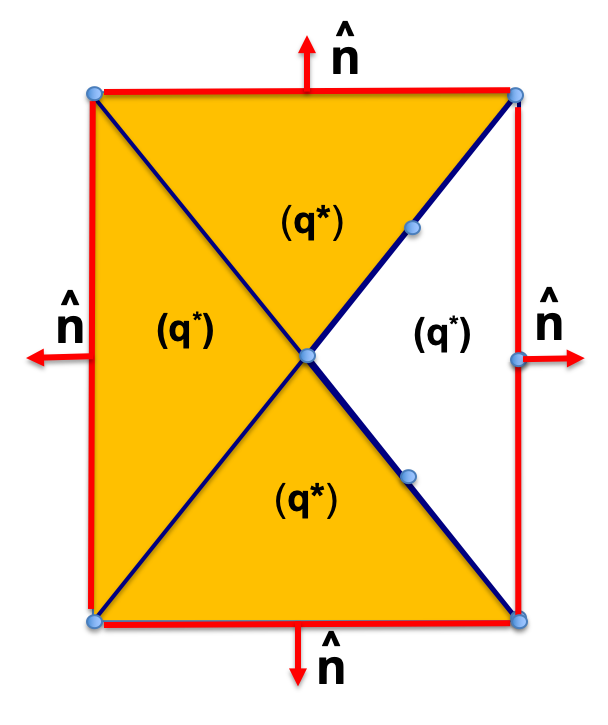
\includegraphics[width=.5\textwidth]{figures/mtc/grid_cartoon_normals.png}
%    %    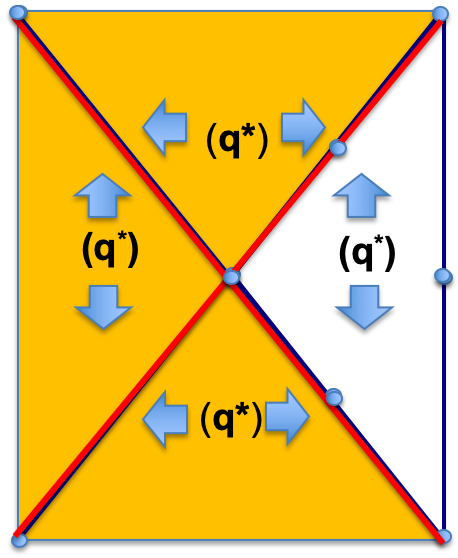
\includegraphics[width=.5\textwidth]{figures/mtc/grid_cartoon_6.png}
%  \end{multicols}
%\end{frame}

%\begin{frame}\frametitle{DG Support - Sub-discretizations (dd)}
%  \begin{multicols}{2}
%    \begin{itemize}
%    \item \textit{Grudge} TracePair data structure for element boundary data
%    \end{itemize}
%% *    \inputminted[mathescape,xleftmargin=0.2in]{python}{figures/mtc/tracepair_sample.py}
%    \columnbreak
%    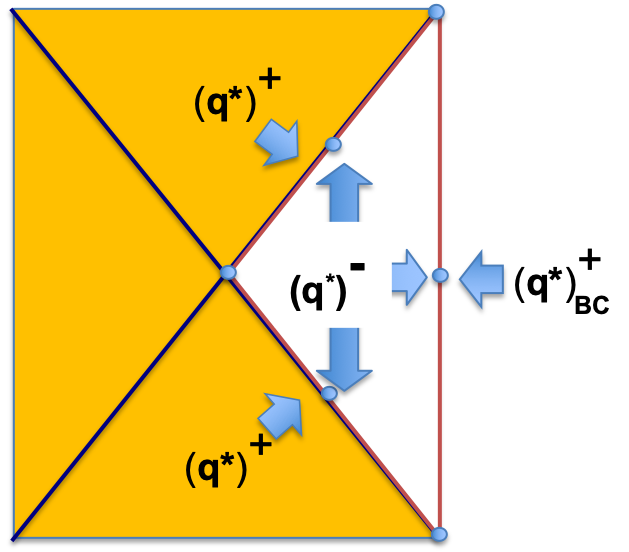
\includegraphics[width=.5\textwidth]{figures/mtc/tracepair_data_cartoon.png}
%  \end{multicols}
%\end{frame}

%\begin{frame}\frametitle{DG Support - Sub-discretizations (dd)}
%  \begin{multicols}{2}
%    \begin{itemize}
%    \item Projections between sub-discretizations: ``vol'' $\rightarrow$ ``int\_faces''
%    \end{itemize}
%    \begin{minted}{python}
%      discr.project("vol", "all_faces", q) 
%    \end{minted}
%    \begin{itemize}
%    \end{itemize}
%    
%    \columnbreak
%    %    %\begin{center}
%    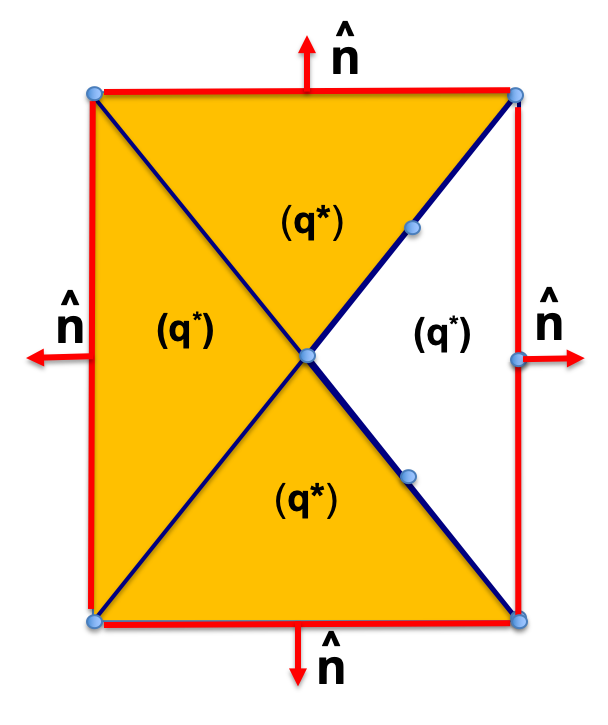
\includegraphics[width=.5\textwidth]{figures/mtc/grid_cartoon_normals.png}
%%    %\end{center}
%  \end{multicols}
%\end{frame}

%\begin{frame}\frametitle{DG Support}
% \begin{multicols}{2}
%\begin{center}
%  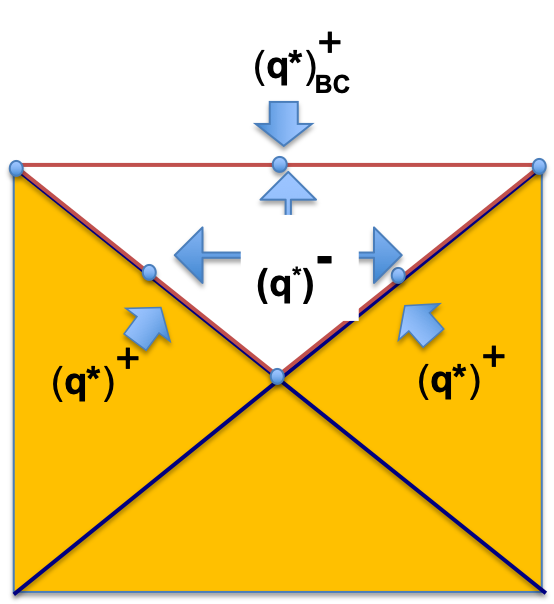
\includegraphics[width=.5\textwidth]{figures/mtc/tracepair_boundaries.png}
%\end{center}
%\end{multicols}
%\end{frame}

% CONS
% Datastructures are a little tough to figure out
% Python - and how it acts on the data structures
% Running afoul of the rules is easy - requires experience
% - some deeper documentation is lacking
% - too hard to discover the rules
% Adding your own kernel C/F90 --> MIRGE
% - mysterious
% Scaling and performance are challenging
%
% PROS
% Follow the rules, and everything works great
% - GPUs, MPI, DG
% Very easy to go from concept and model to working simulation


%\begin{frame}\frametitle{Oustanding issues with mixtures \& combustion}
%\begin{itemize}
%\item Providing a sane starting temperature for Newton iterations
%\begin{itemize}
%\item Use temperature from the last step (prototype in-testing)
%\item Tough to do (right) in lazy-eval 
%\end{itemize}
%\end{itemize}
%\end{frame}

%\begin{frame}\frametitle{\textit{Prometheus} EOS}
%\begin{multicols}{2}
%\begin{itemize}
%   \item Interface functions
%   \begin{itemize}
%      \item get\_temperature(e, Y, Tguess) $\rightarrow (T, Cp_{mix}, R_{mix})$
%      \item get\_pressure(Y, T) $\rightarrow P_{mix}$ 
%      \item get\_mix\_cp(T, Y) $\rightarrow (Cp_{mix})$ 
%      \item get\_mix\_cv(T, Y) $\rightarrow (Cv_{mix})$
%      \item get\_mix\_e(T, Y) $\rightarrow (e)$
%      \item get\_mix\_enthalpy(T, Y) $\rightarrow (h_{mix})$
%      \item get\_species\_cp\_R(T) $\rightarrow (Cp_{i})$ 
%      \item get\_species\_enthalpies(T, Y) $\rightarrow (h_{i})$
%   \end{itemize}
%   \item Wrap interface to \textit{mirgecom} standard EOS - small to medium effort
%   \item Special considerations
%   \begin{itemize}
%      \item Species ordering, naming
%      \item Buffer species handling
%   \end{itemize}
%   \item Potential tests:
%   \begin{itemize}
%     \item Species-specific mixture tests (i.e. one species-at-a-time)
%     \item Calorically perfect mixture - Compare Prometheus vs. \textit{mirgecom}@CPEOS
%     \item Thermally perfect mixture with linear $Cp_i$ - test temperature inversion vs. analytic? 
%   \end{itemize}
%\end{itemize}
%\end{multicols}
%\end{frame}

%\begin{frame}\frametitle{Wrappers for \textit{Prometheus} EOS}
%Create \textit{mirgecom}-EOS-compatible wrappers for \textit{Prometheus} interface functions.
%\begin{itemize}
%\item get\_pressure(state)
%\item get\_temperature(state)
%\item get\_internal\_energy(state)
%\item get\_speed\_of\_sound(state)
%\end{itemize}
%\end{frame}

%\begin{frame}\frametitle{\textit{Prometheus} chemistry \& transport}
%\begin{itemize}
%\item Chemistry - get\_net\_production\_rates($\rho$, T, Y) $\rightarrow (\dot{\omega}_i)$
%\item For explicit integration - directly feeds species source terms $S_i = (W_i \dot{\omega}_i)$
%\item Transport
%   \begin{itemize}
%      \item Species:  $(\kappa_i, \mu_i, D_{ij})$
%      \item Mixture: $(\kappa, \mu, D_i)$
%   \end{itemize}
%\end{itemize}
%\end{multicols}
%\end{frame}

%\begin{frame}\frametitle{Integrating \textit{Prometheus} into \textit{mirgecom}}
%There are 4 \textit{Prometheus} constructs to consider for integration:
%\begin{itemize}
%\item Mechanism generation
%\item Equation of state (EOS)
%\item Chemistry
%\item ``Advanced'' transport (future)
%\end{itemize}
%\end{frame}
%\begin{frame}\frametitle{Performance expectations?}
%\begin{itemize}
%\item Difficult to know what to expect for lazy eval 
%\item Eager - we can probably make a reasonable rough count
%\end{itemize}
%\end{frame
\begin{frame}\frametitle{Daily ASC Platform Tests (Older)}
  %    \vspace{0pt}
  \setlength{\columnsep}{-7.0cm}
  \begin{multicols}{2}
    \begin{minipage}{.2\textwidth}
      \vspace{1cm}
      \hspace{-2cm}
    \begin{itemize}
    \item Lassen GPUs%\hspace{-2cm}%
    \item 1(+) times daily cron
    \item Exercises and times key capabilities
    \end{itemize}
    \end{minipage}
    \columnbreak
    \hspace{-80pt}
    \begin{figure}[htpb]
      \includegraphics[width=.6\textwidth]{figures/mtc2/nozzle_timing_full.pdf}
    \end{figure}		
  \end{multicols}
  \vspace{0pt}
  \begin{tikzpicture}[remember picture, overlay]
    \fill <2> [fill=white, opacity=0.8] (current page.south west) + (0.5,0.5) rectangle (13, 8);
    \node <2> [inner sep=0pt] at (current page.center) {
      \includegraphics[width=.7\textwidth]{figures/mtc2/nozzle_timing_detail.pdf}
    };
  \end{tikzpicture}
  % make a grid:
  % \tikz[overlay, remember picture, help lines]{
  %   \foreach \x in {0,...,12} \path (current page.south west) +(\x,9.25) node {\small$\x$};
  %   \foreach \y in {0,...,9} \path (current page.south west) +(12.5,\y) node {\small$\y$};
  %   \foreach \x in {0,0.5,...,12.5} \draw (current page.south west) ++(\x,0) -- +(0,9.6);
  %   \foreach \y in {0,0.5,...,9.5} \draw (current page.south west) ++(0,\y) -- +(12.8,0);
  % }
  %
\end{frame}

\begin{frame}\frametitle{Daily ASC Platform Tests (Newer)}
  %    \vspace{0pt}
  \setlength{\columnsep}{-7.0cm}
  \begin{multicols}{2}
    \begin{minipage}{.2\textwidth}
      \vspace{1cm}
      \hspace{-2cm}
    \begin{itemize}
    \item Lassen GPUs%\hspace{-2cm}%
    \item 1(+) times daily cron
    \item Exercises and times key capabilities
    \end{itemize}
    \end{minipage}
    \columnbreak
    \hspace{-80pt}
    \begin{figure}[htpb]
      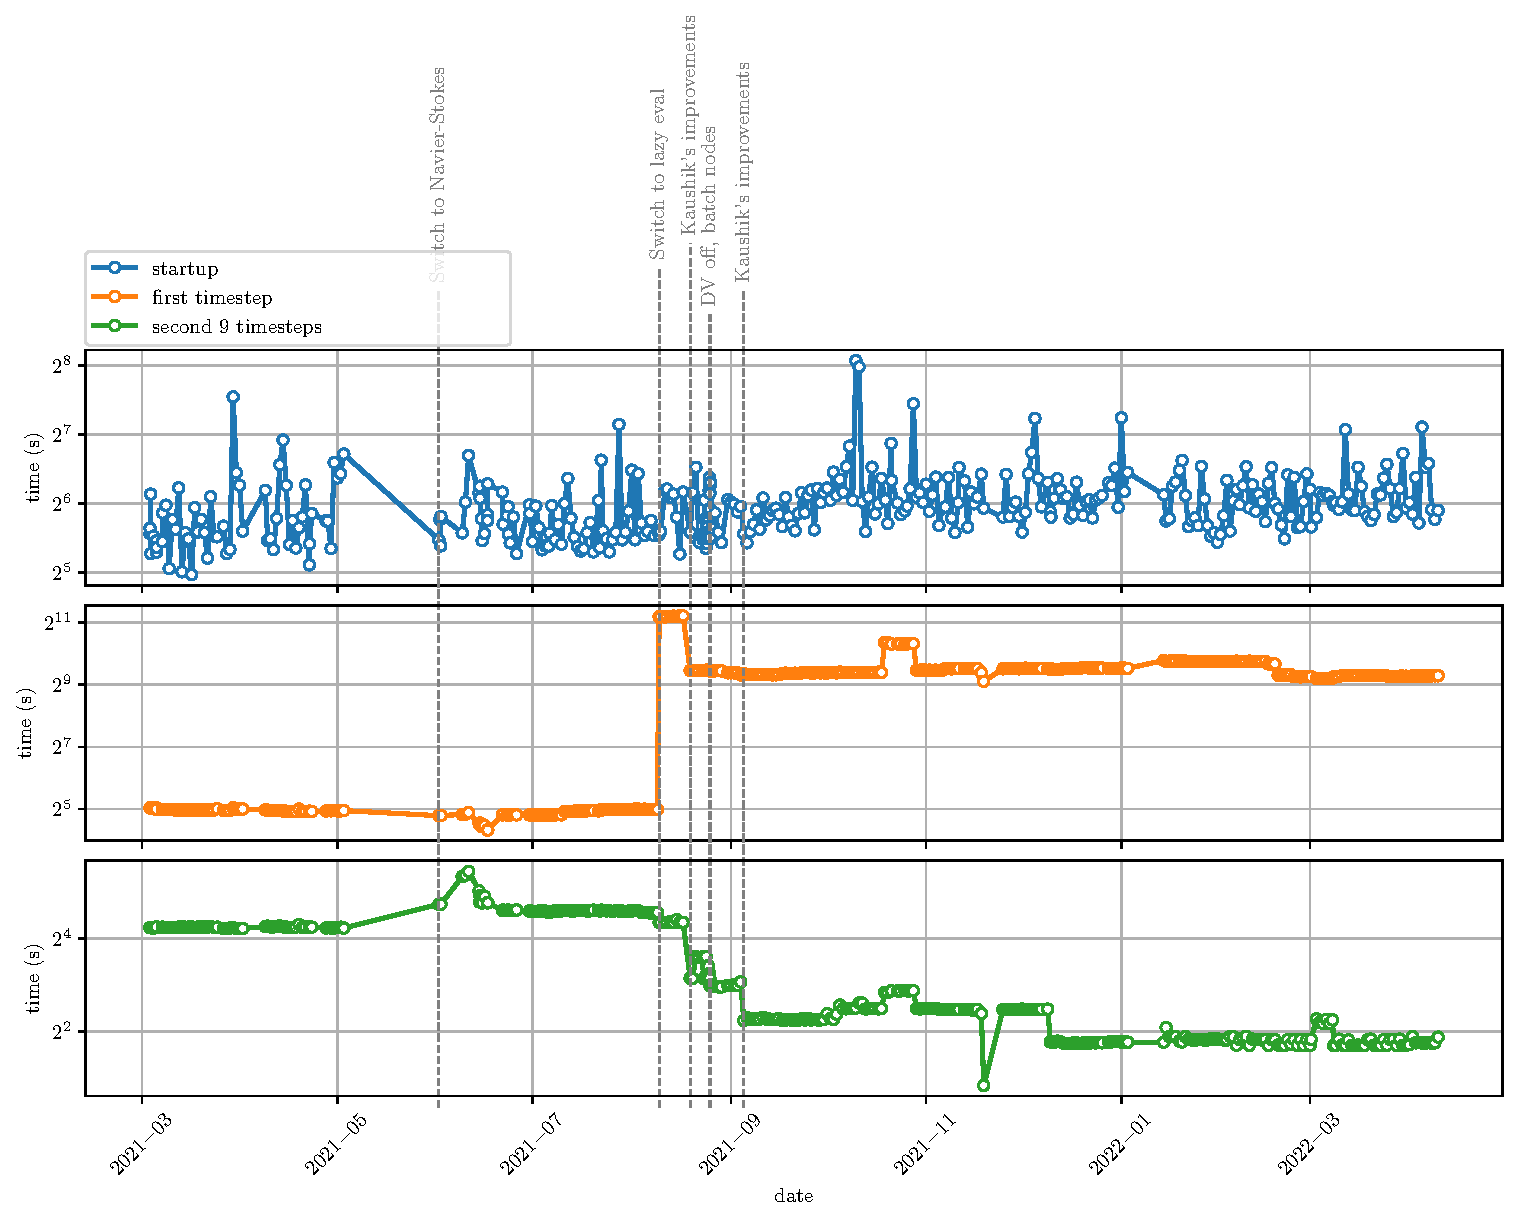
\includegraphics[width=.6\textwidth]{figures/mtc2/nozzle-lazy-full.pdf}
    \end{figure}		
  \end{multicols}
  \vspace{0pt}
  \begin{tikzpicture}[remember picture, overlay]
    \fill <2> [fill=white, opacity=0.8] (current page.south west) + (0.5,0.5) rectangle (13, 8);
    \node <2> [inner sep=0pt] at (current page.center) {
      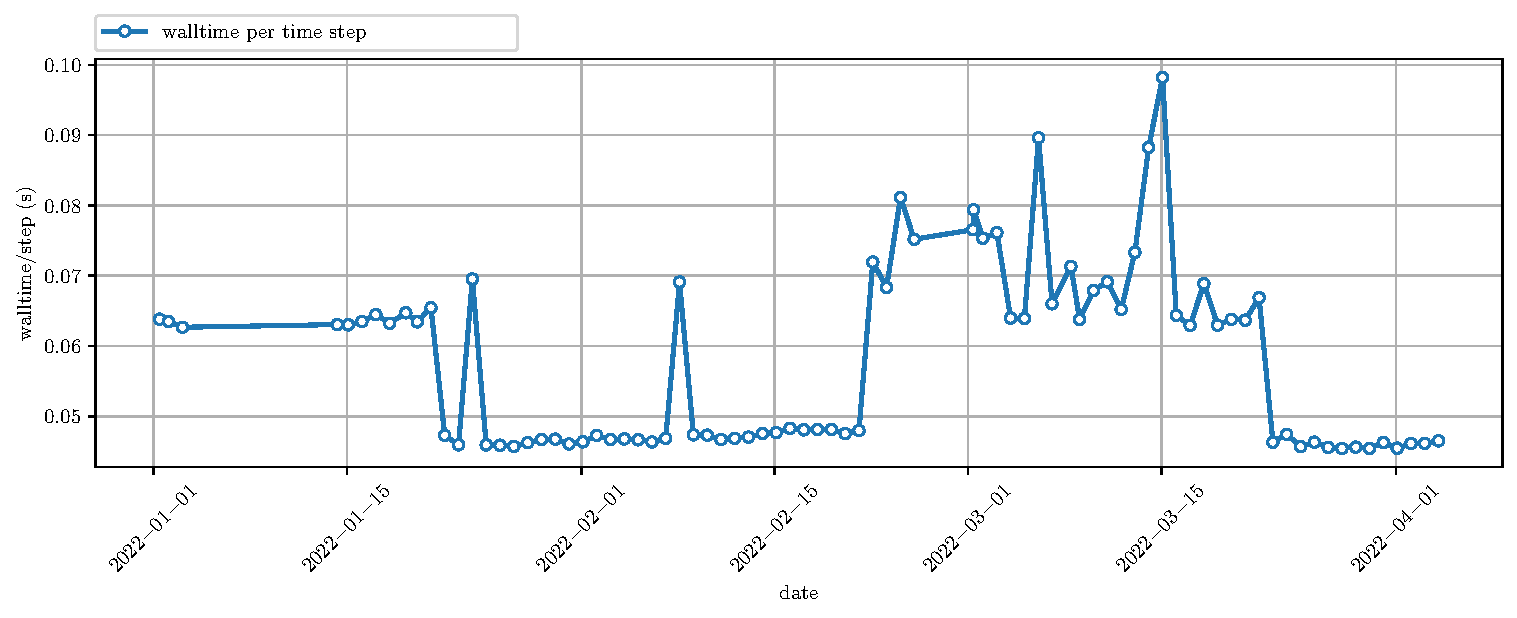
\includegraphics[width=.7\textwidth]{figures/mtc2/isolator-history-zoom.pdf}
    };
  \end{tikzpicture}
  % make a grid:
  % \tikz[overlay, remember picture, help lines]{
  %   \foreach \x in {0,...,12} \path (current page.south west) +(\x,9.25) node {\small$\x$};
  %   \foreach \y in {0,...,9} \path (current page.south west) +(12.5,\y) node {\small$\y$};
  %   \foreach \x in {0,0.5,...,12.5} \draw (current page.south west) ++(\x,0) -- +(0,9.6);
  %   \foreach \y in {0,0.5,...,9.5} \draw (current page.south west) ++(0,\y) -- +(12.8,0);
  % }
  %
\end{frame}


%\begin{frame}\frametitle{Combozzle GPU utilization on Lassen}
%\begin{itemize}
%\item 100k 3rd order elements, RK4, UIUC mech
%\item Using \textit{nvidia-smi}, \textit{nvprof}
%\item Illustrating single timestep scale
%\begin{minipage}{1.0\textwidth}
% %\begin{figure}
%  %\centering
%  \begin{center}
%    % \hspace{-15pt}
%    \includegraphics[width=.35\textwidth]{figures/mtc2/GPUtilizationEager2.png} 
%    \includegraphics[width=.35\textwidth]{figures/mtc2/GPUtilizationLazy2.png}
%  \end{center}
%%    \end{figure}		
%  \end{minipage}
%\begin{minipage}{1.0\textwidth}
% %\begin{figure}
%  %\centering
%  \begin{center}
%  %\hspace{-15pt}
%  \includegraphics[width=.35\textwidth]{figures/mtc2/GPUMemEager.png} 
%  \includegraphics[width=.35\textwidth]{figures/mtc2/GPUMemLazy.png}
%  \end{center}
%%    \end{figure}		
%  \end{minipage}
%\end{itemize}
%%  \begin{tikzpicture}[remember picture, overlay]
%%    \fill <2> [fill=white, opacity=0.7] (current page.south west) + (0.5,0.5) rectangle (12.5, 7.5);
%%    \node <2> [inner sep=0pt] at (current page.center) {
%%      \includegraphics[width=.6\textwidth]{figures/mtc2/StepperSnippet.png}
%%    };
%%  \end{tikzpicture}
%\end{frame}

%\begin{frame}\frametitle{Cost of mixtures}
%\begin{itemize}
%\item What does it cost to turn on mixtures?
%\begin{itemize}
%    \item For full combozzle, lazy $\sim$ factor-of-3 on Lassen GPU
%    \item For eager, it depends on Newton step in \texttt{get\_temperature}
%    \item Lazy autoignition ($\approx$ 300 elements) is well below the ``floor'' 
%\end{itemize}
%\end{itemize}
%\begin{center}
%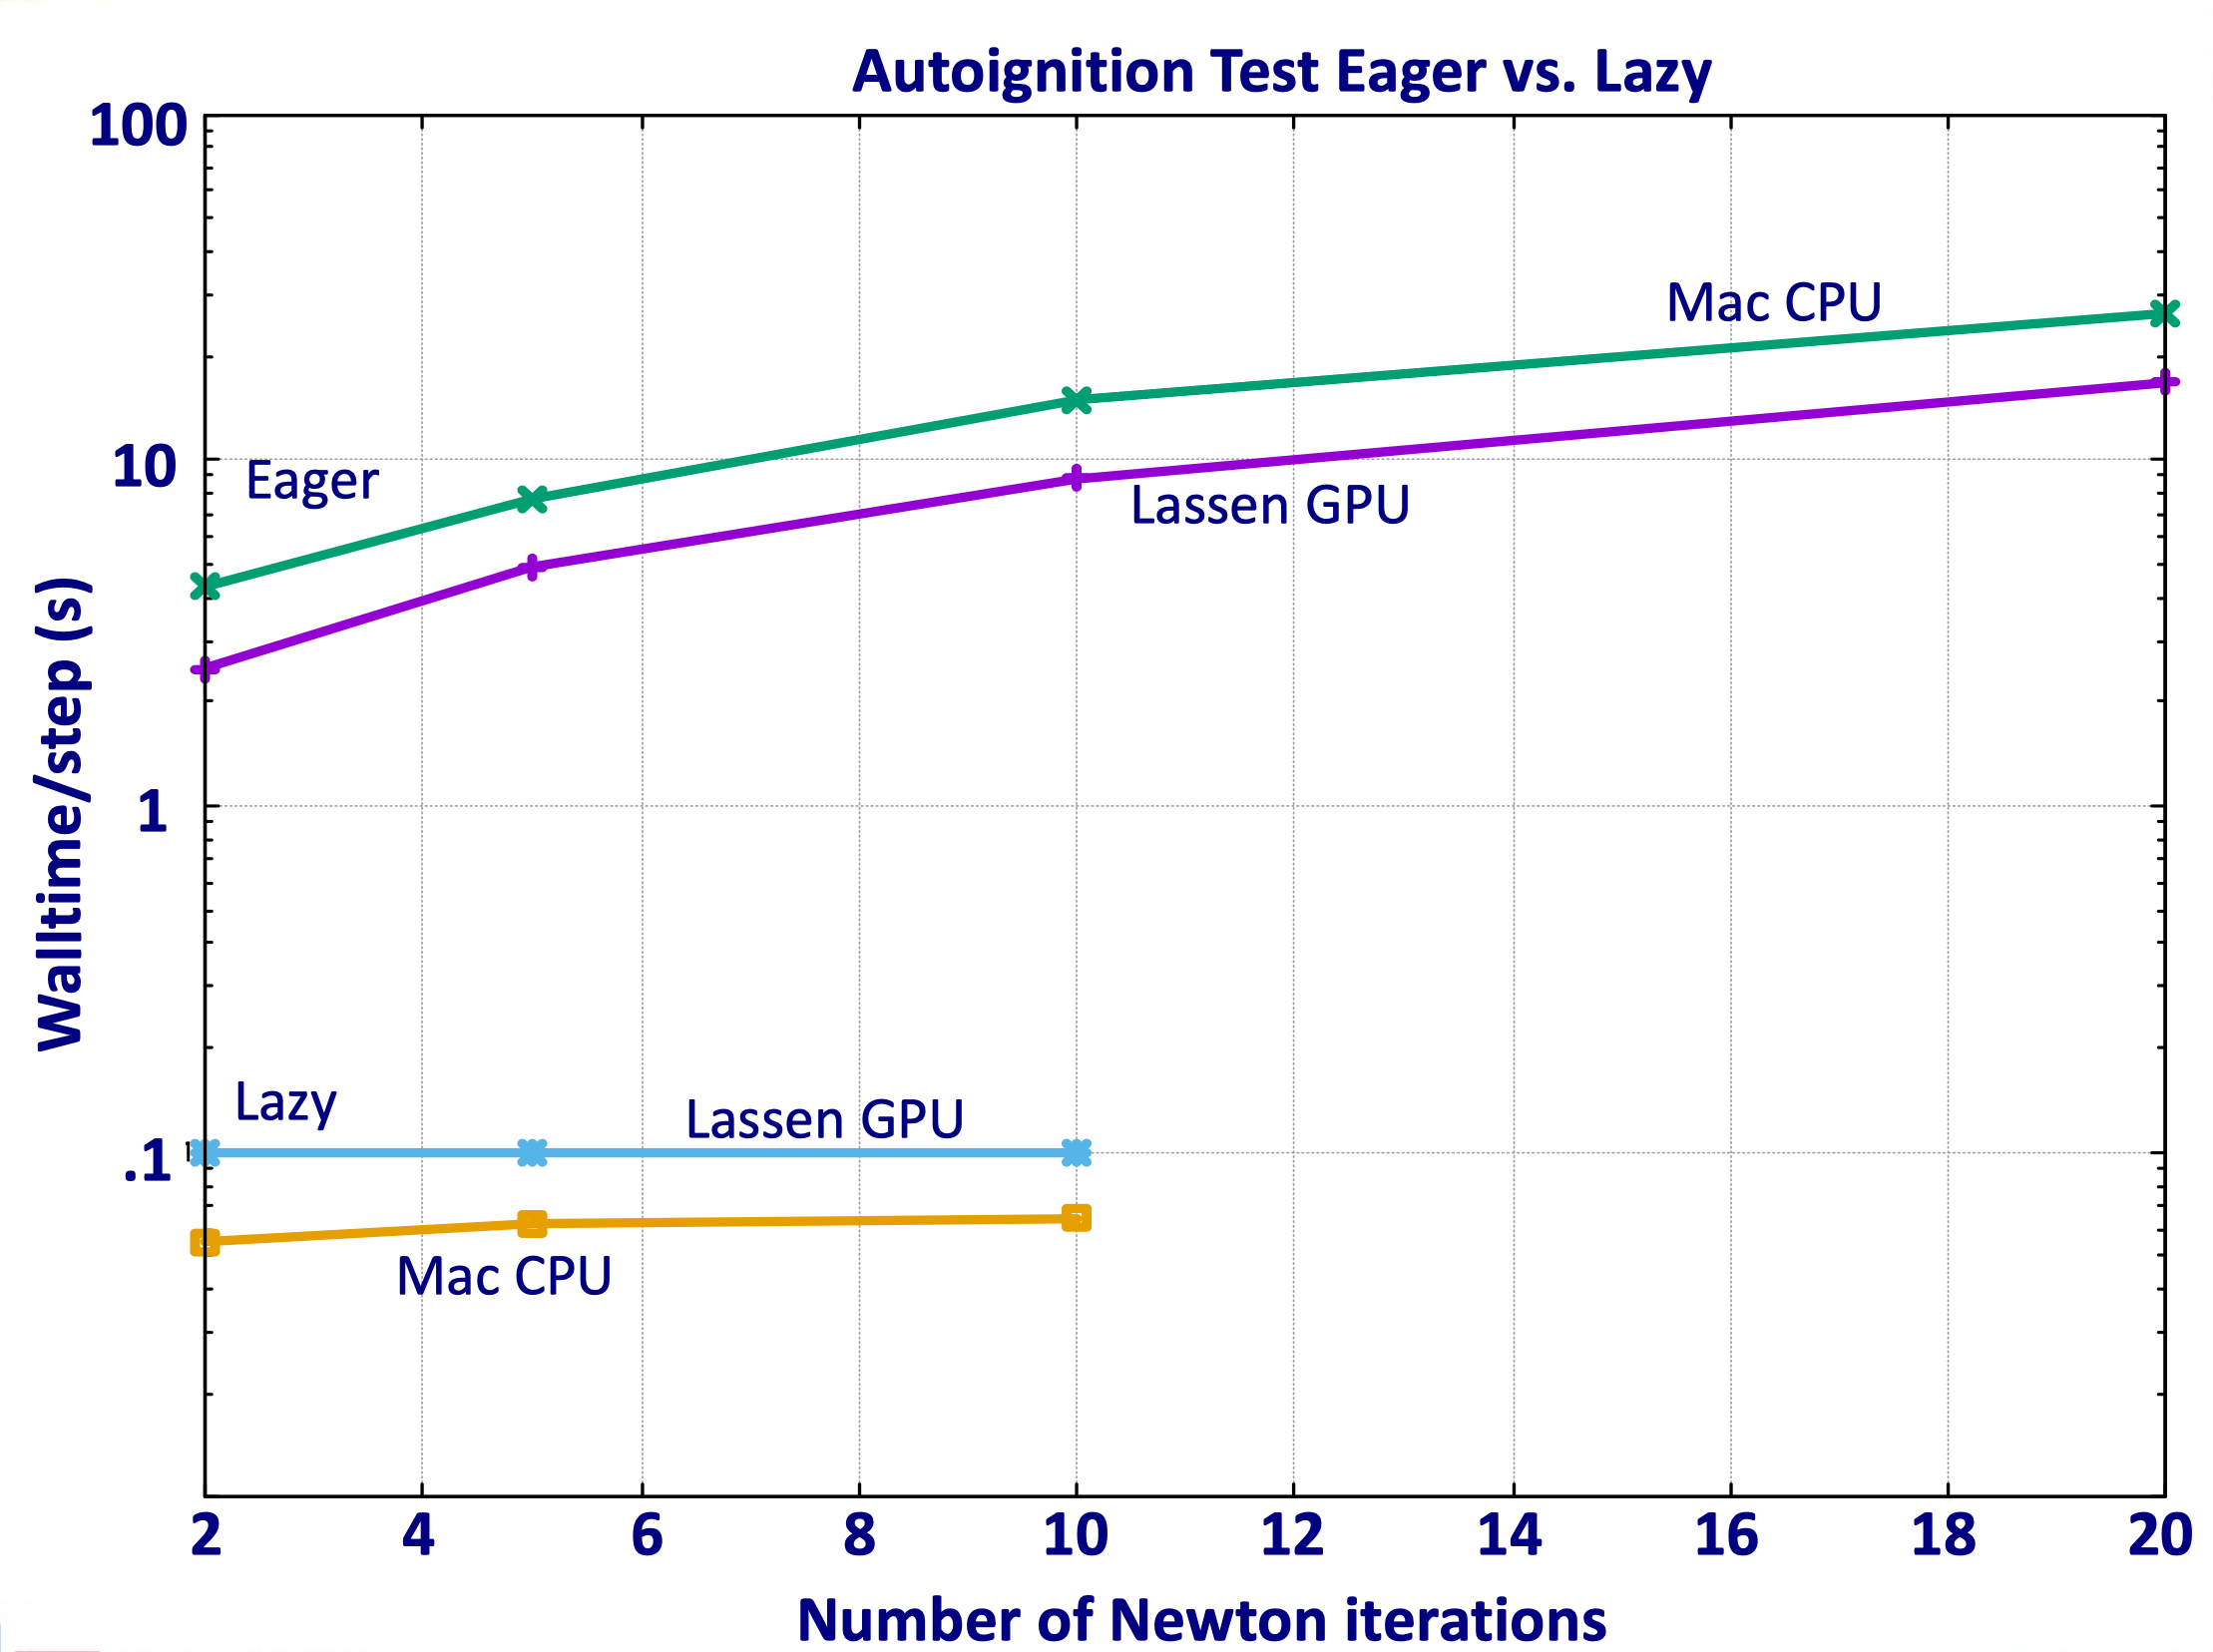
\includegraphics[width=.7\textwidth]{figures/mtc2/AutoignitionNewtonTest2.png}
%\end{center}
%\end{frame}


%\begin{frame}\frametitle{Prediction needs}
%\begin{center}
%Estimates of prediction resources required based on Combozzle performance
%\end{center}
%\begin{multicols}{2}
%\begin{itemize}
%\item Production target
%\begin{itemize}
%\item 100M 3D, p=3 (20 DOFs/element/eqn)
%\item 7-species C2H4 mechanism (12 eqns)
%\item 24B total DOFs
%\item Probably: NS, AV, sponge (Nozzle-like physics)
%\item Probably: $ns$-scale RK4 timesteps
%\item 60$\mu$s per flow-through
%\end{itemize}
%\item Februrary pilot run:
%\begin{itemize}
%\item Surprise: Issue with mixture species at walls
%\item Surprise: Lazy eval failed on targeted cases
%\end{itemize}
%\end{itemize}
%\columnbreak
%\begin{itemize}
%\item Distributed (multi-GPU) lazy will be required 
%\item Minimum production resource: 200 Lassen nodes
%\begin{itemize}
%\item 125K elements/GPU
%\item 2.5s/step $\rightarrow$ 2 days/flow-through
%\end{itemize}
%\item Machine-scale resource: 600 Lassen nodes
%\begin{itemize}
%\item 42K elements/GPU
%\item 1s/step $\rightarrow$ 17h/flow-through
%\end{itemize}
%\end{itemize}
%\end{multicols}
%\end{frame}

\begin{frame}\frametitle{What happened?}
\begin{multicols}{2}
\begin{itemize}
\item Physics issues:
      \begin{itemize}
      \item Inert run: instabilities and unexplained features (ESDG/limiting?)
      \item Combustion (and switch to): unevaluated 
      \item Wall coupling: unevaluated
      \end{itemize}
\item Infrastructure issues:
      \begin{itemize}
      \item Mesh > 30M elements: DNC/OOR
      \item Performance:
            \begin{itemize}
            \item 30M elements: 22s/timestep
            \item time/step increasing with compute resources
            \end{itemize}
      \item Restart on different mesh/partitioning: unevaluated
      \end{itemize}
\end{itemize}
\columnbreak
\begin{figure}
\centering
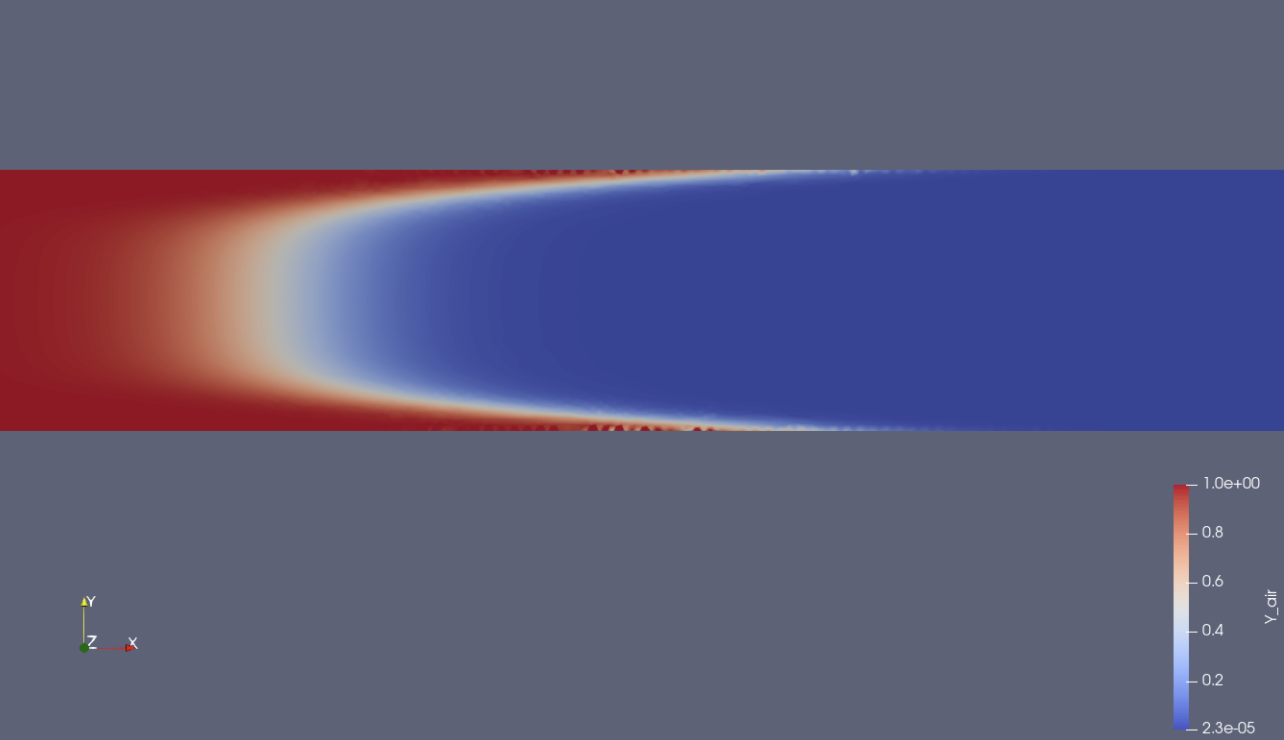
\includegraphics[width=.4\textwidth]{figures/y_unstable_1.png} \\
\includegraphics[width=.4\textwidth]{figures/y_unstable_2.png}
\end{figure}		
\end{multicols}
\end{frame}

\begin{frame}\frametitle{Why were we surprised?}
\begin{multicols}{2}
\begin{itemize}
\item We prepared:
\begin{itemize}
\item The team worked hard to get \mirgecom{} into shape for the February runs
\item Many ``representative'' test cases were excercised at prediction-relevant scales
\item Capabilities were developed, refined, exercised and tested (to some extent)
\item We had every indication that the runs would ``just work''
\end{itemize}
\end{itemize}
\columnbreak
\begin{itemize}
\item But it turns out:
\begin{itemize}
\item Our prep-and-test cases are not really ``representative'' (physics, and mesh)
\item Preparation efforts were not sync'd across the team (we didn't agree on \textit{representative})
\item Capability tests are not sufficient to rule-out broken features
\end{itemize}
\end{itemize}
\end{multicols}
\end{frame}

\begin{frame}\frametitle{Why were we surprised?}
\begin{multicols}{2}
\begin{itemize}
\item We prepared:
\begin{itemize}
\item The team worked hard to get \mirgecom{} into shape for the February runs
\item Many ``representative'' test cases were excercised at prediction-relevant scales
\item Capabilities were developed, refined, exercised and tested (to some extent)
\item We had every indication that the runs would ``just work''
\end{itemize}
\end{itemize}
\columnbreak
\begin{itemize}
\item But it turns out:
\begin{itemize}
\item Our prep-and-test cases are not really ``representative'' (physics, and mesh)
\item Preparation efforts were not sync'd across the team (we didn't agree on \textit{representative})
\item Capability tests are not sufficient to rule-out broken features
\end{itemize}
\end{itemize}
\end{multicols}
\center{Issue: Insufficient V\&V for prediction capabilities (physics and infrastructure)}
\end{frame}

\begin{frame}\frametitle{Minimizing surprise for the prediction}
\begin{multicols}{2}
\begin{itemize}
\item Increase awareness of prediction capability gaps
      \begin{itemize}
      \item Test suite repo  % For prediction capabilities
      \item Performance for prediction-relevant cases
      \item Capability status grid
      \end{itemize}
\item Development and debugging viscosity
      \begin{itemize}
      \item More test documentation/standardization
      \item Driver refactor, cleanup, simplification
      \item Reduction of unmerged capabilities
      \item Development process review and evolution
      \item Team experience dissemination (debugging, etc)
      \end{itemize}
\end{itemize}
\columnbreak
\includegraphics[width=.5\textwidth]{figures/PredictionCapabilityStatusChart.png}
\end{multicols}
\end{frame}

%\begin{frame}\frametitle{Summary of prediction capability gaps}
%\begin{itemize}
%\item Infrastructure gaps (Matthias today)
%      \begin{itemize} 
%      \item Mesh > 30M: Out of resources
%      \item Prohibitive performance: 22s/step inert (order of magnitude)
%      \item Performance goes down with increasing resources
%      \item Change mesh/partitioning on restart?
%      \end{itemize}
%\item Physics gaps
%      \begin{itemize}
%      \item Wall model and coupling (Matt today)
%      \item Issues with species handling at boundaries
%      \item Potential issue with boundary layer thickness
%      \item Observed negative mass fractions in the volume
%            \begin{itemize}
%            \item Need ESDG?
%            \item Species limiting?
%            \end{itemize}
%      \item 3D case not stable?
%      \item Combustion?
%      \item Switch inert run to mixture?
%      \end{itemize}
%\end{itemize}
%\end{frame}


\begin{frame}\frametitle{Existing \mirgecom{} V\&V testing for physics}
\begin{multicols}{2}
\begin{itemize}
\item Unit example: Poiseuille
\item Integrated example: Pyro/combustion verif
\item New tests: \prj{\tiny}{T. Ricciardi}
\item Address needs:
      \begin{itemize}
      \item Documentation, organization, standardization? of our current testing
      \item More tests (of course):
            \begin{itemize}
            \item Prediction-relevant capability tests
            \item Prediction-relevant issue reproducers,
            \item and manufactured solution tests
            \end{itemize}
      \end{itemize}
\end{itemize}
\columnbreak
\includegraphics[width=.4\textwidth]{figures/PoiseuilleConvergence2.png}
\includegraphics[width=.4\textwidth]{figures/autoignition_temperature.pdf}
%\includegraphics[width=.48\textwidth]{figures/PyroVerif2.png}
\end{multicols}
  \begin{tikzpicture}[remember picture, overlay]
    \fill <2> [fill=white, opacity=0.8] (current page.south west) + (0.5,0.5) rectangle (12.5,7.5);
    \node <2> [inner sep=0pt] at (current page.center) {
      \includegraphics[width=.75\textwidth]{figures/ExamplesReadme.png}
    };
  \end{tikzpicture}
\end{frame}

\begin{frame}\frametitle{Existing \mirgecom{} V\&V testing for physics}
\begin{multicols}{2}
\begin{itemize}
\item Unit example: Poiseuille
\item Integrated example: Pyro/combustion verif
\item New tests: \prj{\tiny}{T. Ricciardi}
\item Address needs:
      \begin{itemize}
      \item Documentation, organization, standardization? of our current testing
      \item More tests (of course):
            \begin{itemize}
            \item Prediction-relevant capability tests
            \item Prediction-relevant issue reproducers,
            \item and manufactured solution tests
            \end{itemize}
      \end{itemize}
\end{itemize}
\columnbreak
\includegraphics[width=.4\textwidth]{figures/PoiseuilleConvergence2.png}
\includegraphics[width=.4\textwidth]{figures/autoignition_temperature.pdf}
%\includegraphics[width=.48\textwidth]{figures/PyroVerif2.png}
\end{multicols}
\end{frame}

\begin{frame}\frametitle{Symbolic infrastructure for fluids}
  \begin{center}
  %Evolution equation:
  Navier--Stokes for reactive mixtures:
  \begin{equation*}
    \frac{\partial\mathbf{Q}}{\partial{t}} + \nabla \cdot (\mathbf{F}^I - \mathbf{F}^V) - \mathbf{S} = 0
  \end{equation*}
  % With chemistry source terms:
  % \begin{equation*}
  %  \mathbf{S} = [ 0, 0, 0, 0, 0, W_k\dot{\omega_k} ]
  %\end{equation*}
    Where state vector $\mathbf{Q}$, fluxes $\mathbf{F}^I$, $\mathbf{F}^V$ , and sources $\mathbf{S}$ are given by:
 \begin{equation*}
      \begin{bmatrix}
        \rho\\\rho{E}\\\rho\vec{v}\\\rho{Y}_\alpha\end{bmatrix},\quad
      \begin{bmatrix} \rho\vec{v}\\(\rho{E} +
        p)\vec{v}\\\rho(\vec{v} \otimes \vec{v}) +
        p\delta_{ij}\\\rho{Y}_\alpha\vec{v}\end{bmatrix}, \quad
       \begin{bmatrix} 0\\(\mathbf{\tau} \cdot \vec{v} - \mathbf{q})\\\mathbf{\tau}_{:j}\\-\mathbf{J}_\alpha\end{bmatrix},\quad
       \begin{bmatrix} 0\\0\\0\\W_\alpha\dot{\omega}_\alpha\end{bmatrix},
 \end{equation*}
with $\tau = \mu\left(\nabla\vec{v} + (\nabla\vec{v})^T\right) + \left(\mu_b - \frac{2\mu}{3}\right)\left(\nabla \cdot \vec{v}\right)$,\\
\vspace{5pt}
$\mathbf{J}_\alpha = -\rho d_{(\alpha)} \nabla(Y_\alpha)$, and $\mathbf{q} = -\kappa\nabla{T}$\\
\vspace{10pt}
    The mixture gas model (EOS) provides $\rightarrow~~(p,T,e,\mu,\kappa,d_{\alpha}, \omega_\alpha)(\mathbf{Q})$
  \end{center}
  \begin{tikzpicture}[remember picture, overlay]
    \fill <2> [fill=white, opacity=0.8] (current page.south west) + (0.5,0.5) rectangle (12.5,7.5);
    \node <2> [inner sep=0pt] at (current page.center) {
      \includegraphics[width=.75\textwidth]{figures/SymbolicInfrastructureCode.png}
    };
  \end{tikzpicture}
\end{frame}

\begin{frame}\frametitle{Symbolic infrastructure for fluid component testing}
\center{What's it good for?}
\begin{itemize}
\item For fluid component verification testing
\item Specify analytic test functions and 
\item Evaluate convergence of MIRGE components to exact/analytic solution
\end{itemize}
\includegraphics[width=\textwidth]{figures/ComponentVerifCode.png}
\begin{itemize}
\vspace{-10pt}
\item and ... method of manufactured solutions (MMS)
\end{itemize}
\end{frame}

\begin{frame}\frametitle{Method of Manufactured Solutions in \mirgecom{}}
\begin{itemize}
\item Craft a solution ($\phi_{*}$) to the conservation system, $\text{CV}_\text{sym}: = \left[\rho=\phi_m, \rho{E}=\phi_e, \rho\mathbf{V}=\mathbf{\phi}_p\right]$, s.t. each component of $\phi_{*}$ is a smooth, continuous function:
\end{itemize}
\includegraphics[width=.8\textwidth]{figures/CreateSymbolicSolution.png}
\begin{itemize}
\item Hit $\text{CV}_\text{sym}$ with the governing equations to find the source terms, $S_\text{sym}$, that generate $\text{CV}_\text{sym}$:
\end{itemize}
\includegraphics[width=.8\textwidth]{figures/CalculateSymbolicSources.png}
\begin{itemize}
\item Modify the implementation of the governing equations by adding the numerical/evaluated sources $S_\text{num}$ to the RHS:
\end{itemize}
\includegraphics[width=.8\textwidth]{figures/NumRHS.png}
\begin{itemize}
\item Evaluate convergence and accuracy at multiple mesh resolutions with
      \begin{itemize}
      \item Soln initialized to numerical $\text{CV}_\text{sym}$, and
      \item Exact/analytic prescribed boundary conditions
      \end{itemize}
\end{itemize}
%\item Advantages:
%      \begin{itemize}
%      \item Simplicity (easily understood and implemented)
%      \item Exercises selected, or all terms
%      \item Tests the whole code - all components in an integrated fashion - component-only tests leave many questions and holes
%      \item Highly sensitive for detecting mistakes
%      \end{itemize}
%\end{itemize}
\end{frame}

\begin{frame}\frametitle{Status of MMS in \mirgecom{}}
%\begin{multicols}{2}
\begin{itemize}
\item Symbolic infrastructure for CNS and Euler
\item Supports multiple scalar components
\item Full MMS test is all but time integration loop
\item Mixture support (symbolic EOS, transport) planned
\item Plan to use MMS to test species boundary treatments:
      \begin{itemize}
      \item Craft $\phi_y$ s.t. $\nabla{Y} \cdot \hat{\mathbf{n}} = 0$
      \end{itemize}
      Example: $\phi_y = \cos(x)\cos(y)$, on $\left[-\pi, \pi\right]^N$
      \begin{itemize}
      \item Evaluate convergence using \mirgecom{} boundaries, *not* exact
      \end{itemize}
\end{itemize}
\end{frame}

\begin{frame}\frametitle{Status of MMS in \mirgecom{}}
\begin{itemize}
\item Roy, Verification of a Compressible CFD Code using the Method of Manufactured Solutions, AIAA Paper 2002-3110 (https://doi.org/10.2514/6.2002-3110)
\end{itemize}
\begin{center}
\includegraphics[width=.75\textwidth]{figures/RoySoln.png}
\end{center}
\end{frame}

\begin{frame}\frametitle{Status of MMS in \mirgecom{}}
\begin{itemize}
\item Ulerich, A Transient Manufactured Solution For the Compressible Navier-Stokes Equations With a Power Law Viscosity, 10th World Congress on Computational Mechanics (DOI:10.5151/meceng-wccm2012-16661)
\end{itemize}
%\end{multicols}
\includegraphics[width=\textwidth]{figures/MoserIISoln.png}
\end{frame}


\begin{frame}\frametitle{Simulation Infrastructure: Driver and Timestepping}
  \begin{multicols}{2}
    \begin{itemize}
    \item Driver provides:
      \begin{itemize}
      \item Configuration
      \item State initialization
      \item Boundaries (\& treatments)
      \item Stepper callbacks (I/O)
      \item Simulation RHS
      \end{itemize}
    \end{itemize}
    \vspace{30pt}
    \begin{center}
      \includegraphics[width=0.2\textwidth]{figures/mtc2/TypicalDriverKeyOrange.png}
    \end{center}
    \columnbreak
    \includegraphics[width=0.4\textwidth]{figures/mtc2/TypicalDriverOrange.png}\\
    \includegraphics[width=0.4\textwidth]{figures/mtc2/TimesteppingAndDriver.png}
  \end{multicols}
\end{frame}


\begin{frame}\frametitle{Summary}
\begin{center}
% Upshot
\begin{itemize}
\item We were surprised by the difficulties in Feb runs
%\item The difficulties themselves are on-par with our endeavor
\item Difficulties/surprise cannot be prevented, but can be controlled (to some extent)
\item Y2 needs:
%\end{itemize}
\begin{multicols}{2}
        \begin{itemize}
        \item Critical: Species@boundary
        \item Critical: Running lazy at scale
        \item Switch to mixture
        \item Power law transport
\columnbreak
        \item Urgent: Wall model/coupling
        \item Urgent: Prohibitive performance
        \item Species mass limiting
        \item ESDG
        \end{itemize}
\end{multicols}
\end{itemize}
%\item Y2 needs (on the near horizon):
%\begin{multicols}{2}
%      \begin{itemize}
%      \columnbreak
%      \end{itemize}
%\end{multicols}
%\end{center}
%Prediction-critical capabilities need to be agreed on, and tracked
%Need increased visibility of prediction-critical capability and their gaps
%Capability development needs to \textit{lead} not \textit{trail} prediction
%\begin{center}
% Plans for filling the process and capability gaps:
\begin{itemize}
\item More and better V\&V testing
      \begin{itemize}
      \item Provides better guardrails on dealing with physics difficulties
      \item Reduces viscosity of capability development by removing uncertainty and fear
      \end{itemize}
\item Prediction capability testing suite
      \begin{itemize}
      \item Specifies prediction capability requirements through tests
      \item Increase awareness of prediction capability gaps
      \item Helps capability development \textit{lead} not \textit{trail} prediction need
      \end{itemize}
\end{itemize}
\end{center}
\end{frame}
